\documentclass[english,titlepage]{uzhpub}
\usepackage[T1]{fontenc}
\usepackage{lmodern}
\usepackage[utf8]{inputenc}

% Math Packages
\usepackage{mathtools} % includes amsmath
\usepackage{amsthm} % for theoremstyle, newtheorem
% TODO: replace \text stuff with these
\DeclareMathOperator\im{im}
\DeclareMathOperator\arctanh{arctanh}
\DeclareMathOperator\arcsinh{arcsinh}
\DeclareMathOperator\arccosh{arccosh}
\usepackage{amsfonts} % for mathbb
\usepackage{amssymb} % for blacksquare
\usepackage{thmtools} % for theorem list
\usepackage{gensymb} % for degree °

% Drawing Packages
\usepackage{pgf}
\usepackage{pgfplots}
\pgfplotsset{compat=1.15}
\usepackage{mathrsfs}
\usepackage{tikz}
\usetikzlibrary{arrows,intersections,angles}
\usepackage{tikz-cd}
\usepackage[customcolors]{hf-tikz}
\usepackage{wrapfig}

\usepackage{xcolor}
\definecolor{black}{HTML}{383838}
\definecolor{grey}{HTML}{787878}
\definecolor{white}{HTML}{D8D8D8}
\definecolor{red}{HTML}{AB4642}
\definecolor{orange}{HTML}{DC9656}
\definecolor{yellow}{HTML}{F7CA88}
\definecolor{green}{HTML}{A1B56C}
\definecolor{cyan}{HTML}{86C1B9}
\definecolor{blue}{HTML}{7CAFC2}
\definecolor{purple}{HTML}{BA8BAF}
\definecolor{brown}{HTML}{A16946}

\usepackage{xr}
\usepackage{enumitem}
\SetLabelAlign{Center}{\hfil(#1)\hfil} % center alignment for enumerate
\usepackage{hyperref}
\usepackage{cleveref}
% LABELLING SCHEME
% ch: chapter
% sec: section
% subsec: subsection
% fig: figure
% tab: table
% eq: equation
% lst: code listing
% itm: enumerated list item
% alg: algorithm
% app: appendix subsection

% def: definition
% thm: theorem
% pro: proposition
% cor: corollary
% lem: lemma

% Formality Packages
\usepackage[toc, nonumberlist]{glossaries}
\makeglossaries
% Foundations
\newglossaryentry{lc}{name=logical connective, description={Aussagenjunktoren}}
\newglossaryentry{qua}{name=quantifier, description={Quantor}}
\newglossaryentry{un}{name=union, description={Vereinigung}}
\newglossaryentry{int}{name=intersection, description={Durchschnitt}}
\newglossaryentry{sub}{name=subset, description={Teilmenge}}
\newglossaryentry{sup}{name=superset, description={Obermenge}}
\newglossaryentry{pow}{name=powerset, description={Potenzmenge}}
\newglossaryentry{relcomp}{name=relative complement, description={Komplement, Differenz}}
\newglossaryentry{compl}{name=complement, description={Symmetrische Differenz}}
\newglossaryentry{quotset}{name=quotient set, description={Restklassenmenge, Quotienten Menge}}
\newglossaryentry{op}{name=operation, description={Verknüpfung}}
\newglossaryentry{inc}{name=increasing, description={wachsend}}
\newglossaryentry{dec}{name=decreasing, description={fallend}}
\newglossaryentry{nest}{name=nested intervals, description={Intervallschachtelung}}
\newglossaryentry{pred}{name=predicate, description={Prädikat}}
\newglossaryentry{disj}{name=disjoint, description={disjunkt}}
\newglossaryentry{preim}{name=pre-image, description={Urbild}}
\newglossaryentry{domain}{name=domain, description={Definitionsbereich}}
\newglossaryentry{codomain}{name=co-domain, description={Zielbereich}}
\newglossaryentry{part}{name=partition, description={(disjunkte) Zerlegung}}
\newglossaryentry{zerodiv}{name=no zero divisors, description={nullteiler freiheit}}

% Algebra
\newglossaryentry{eucl}{name=Euclidean Domain, description={Euklidischer Ring}}
\newglossaryentry{pre-image}{name=pre-image, description={Urbild}}
\newglossaryentry{fibre}{name=fibre, description={Faser}}
\newglossaryentry{wlog}{name=w.l.o.g., description={without loss of generality}}
\newglossaryentry{unit}{name=unit, description={Einheit}}
\newglossaryentry{coprime}{name=coprime, description={teilerfremd}}
\newglossaryentry{gcd}{name=greatest common denominator, description={Grösster gemeinsamer Teiler}}
\newglossaryentry{res}{name=residue class, description={Restklasse}}
\newglossaryentry{span}{name=(linear) span, description={Lineare Hülle}}
\newglossaryentry{transmat}{name=transformation matrix, description={Darstellende Matrix}}
\newglossaryentry{trig}{name=triangularizable, description={trigonalisierbar}}
\newglossaryentry{inv}{name=inversion, description={Fehlstand, Inversion}}
\newglossaryentry{adj}{name=adjugate matrix, description={Adjunkte, komplementäre Matrix}}
\newglossaryentry{path}{name=path-component, description={Wegzusammenhangskomponente}}
\newglossaryentry{tr}{name=trace, description={Spur}}
\newglossaryentry{comp}{name=companion matrix, description={Begleitmatrix}}
\newglossaryentry{ext}{name={Exterior Product}, description={Äussere Potenz}}
\newglossaryentry{sym}{name={Symmetric Power}, description={Symmetrische Potenz}}
\newglossaryentry{outer}{name={Outer Product}, description={Dyadisches-, Tensorielles Produkt}}
\newglossaryentry{dot}{name={Dot Product}, description={Standardskalarprodukt}}
\newglossaryentry{inner}{name={Inner Product}, description={Skalarprodukt}}
\newglossaryentry{axis}{name={Principal Axis Theorem}, description={Hauptachsentransformation}}
\newglossaryentry{adju}{name={self-adjoint}, description={selbstadjungiert}}
\newglossaryentry{sylv}{name={Sylvester's Law of Inertia}, description={Sylvesterscher Trägheitssatz}}
\newglossaryentry{cross}{name={Cross Product}, description={Kreuzprodukt, Vektorprodukt}}
\newglossaryentry{gram}{name={Gram-Schmidt Process}, description={Gram-Schmidtsches Orthogonalisierungsverfahren}}
\newglossaryentry{cos}{name={Law of Cosines}, description={Kosinussatz}}
\newglossaryentry{quot}{name={Quotient-, Factor-, Residue (Class) Ring}, description={Quotientenring, Restklassenring}}
\newglossaryentry{tors}{name={Torsion}, description={Torsion, Torsionsuntermodul}}
\newglossaryentry{cokernel}{name={Cokernel}, description={Kokern}}
\newglossaryentry{ufd}{name={Unique Factorization Domain (UFD)}, description={Faktorieller Ring}}
\newglossaryentry{pid}{name={Principal Ideal Domain (PID)}, description={Hauptidealring}}
\newglossaryentry{solv}{name={solvable group}, description={Auflösbare Gruppe}}
\newglossaryentry{inva}{name={invariant}, description={remain unchanged under changed conditions}}

\glsaddall

% Math styling
\renewcommand\qedsymbol{$\blacksquare$}

\theoremstyle{definition}
\newtheorem{definition}{Definition}[section]

\theoremstyle{plain}
\newtheorem{proposition}[definition]{Proposition}
\newtheorem{lemma}[definition]{Lemma}
\newtheorem{theorem}[definition]{Theorem} % numbered theorem
\newtheorem{corollary}{Corollary}[theorem]

\theoremstyle{remark}
\newtheorem*{remark}{Remark}

\theoremstyle{example}
\newtheorem*{example}{Example}

\begin{document}
   \title{Analysis 1}
   \subtitle{Definitions, Proofs and Examples}
   \author{Tim Bachofen}
   \date{HS 2018}

   \maketitle

   \tableofcontents
   \newpage

   \renewcommand{\listtheoremname}{List of Definitions}
   \listoftheorems[ignoreall, show={definition}]
   \newpage

   \renewcommand{\listtheoremname}{List of Statements}
   \listoftheorems[ignoreall, show={theorem,corollary,proposition,lemma}]
   \newpage

   \section{Foundations}
   \subsection{Motivation for \texorpdfstring{\(\mathbb{R}\)}{R}}
   In \(\mathbb{Q}\) are addition and multiplication invertible, which means it is always possible to solve linear equations.
   In other words, for an arbitrary \(a \in \mathbb{Q} \setminus \{0\}\) and \(b \in \mathbb{Q}\) exists exactly one solution \(x \in \mathbb{Q}\) to the equation \(a \cdot x + b = 0\).

   However already for quadratic equations arises the first problem.

   \begin{theorem}[\(\sqrt{2} \not\in \mathbb{Q}\)]
      \[\not\exists x \in \mathbb{Q}: x^2 = 2\]
   \end{theorem}
   \begin{proof}
      Suppose \(\exists x \in \mathbb{Q}: x^2 = 2\) then \(\exists q \in \mathbb{N} \setminus \{0\}: q \cdot x \in \mathbb{Z}\).
      \[M = \{q \in \mathbb{N}\setminus\{0\}: q \cdot x \in \mathbb{Z}\}\]
      Since \(M \neq \emptyset\), the well-order principle implies that \(M\) has a minimum.

      Let \(g \in M\) be the minimal element and \(p = g \cdot x \in \mathbb{Z}\), then \(x = \frac{p}{g}\) holds.
      \(g\) being the minimal element implies that \(p\) and \(g\) are coprime.
      \[2 = \frac{p^2}{g^2} \implies p^2 = 2 g^2\]
      This implies that \(p^2\) is even.
      Because of that, \(p\) must be even as well (since \((2n + 1)^2 = 4n^2 + 4n + 1\) is always uneven).
      This means that a \(\exists m \in \mathbb{Z}: p = 2m\), then
      \[4m^2 = (2m)^2 = p^2 = 2g^2 \implies g^2 = 2m^2\]
      which means that \(g\) is even as well.
      This leads to a contradiction to the fact that \(g\) and \(p\) are coprime.
   \end{proof}

   \begin{proposition}[\(\sqrt{2} \in \mathbb{R}\)]
      \[\exists c > 0 \in \mathbb{R}: c^2 = 2\]
   \end{proposition}
   \begin{proof}
      Given the bounded above set \(A = \{x \in \mathbb{R}: (x \geq 0) \land (x^2 \leq 2)\}\) and its supremum \(c = \sup A\).

      We assert that \(c^2 = 2\) and now assume that \(c^2 < 2\).
      We choose
      \[0 < \epsilon < \frac{2 - c^2}{2c + 1} \leq 1\]
      \[(c + \epsilon)^2 = c^2 + 2c\epsilon + \epsilon^2 \leq c^2 + (2c + 1)\epsilon \leq 2\]
      Because of this is \((c + \epsilon) \in A\), which leads to the contradiction that \(c\) is an upper bound.

      We proceed by asserting that \(c^2 > 2\).
      We chose
      \[0 < \epsilon < \frac{c^2 - 2}{2c}\]
      \[(c - \epsilon)^2 = c^2 - 2\epsilon c + \epsilon^2 \leq c^2 - 2\epsilon c > 2\]
      This implies that \(c - \epsilon\) is an upper bound of \(A\), which is again a contradiction to that \(c\) is the supremum.

      Hence it holds that \(c^2 = 2\).
   \end{proof}
   \begin{remark}
      Given \(a > 0 \in \mathbb{R}\) and \(p \in \mathbb{N}\setminus 0\)
      \[\exists! x > 0 \in \mathbb{R}: x^p = a\]
   \end{remark}

   \subsection{Construction of \texorpdfstring{\(\mathbb{R}\)}{R}}
   In order to construct the real numbers we first need to introduce some concepts.

   \begin{definition}[Order Complete Set]
      A totally ordered set \((M, \preceq)\) is order complete if the following holds.

      Given the subsets \(A, B \neq \emptyset \subset M\) with \(\forall a \in A, \forall b \in B: a \preceq b\)
      \[\exists c \in M: (\forall a \in A: a \preceq c) \land (\forall b \in B: c \preceq b)\]
   \end{definition}
   \begin{remark}
      \(\mathbb{Q}\) is a totally ordered set but not order complete. Given
      \[A = \{x \in \mathbb{Q}^+: 0 < x \land x^2 < 2\}\]
      \[B = \{x \in \mathbb{Q}^+: 0 < x \land x^2 > 2\}\]
      \[\not\exists c \in \mathbb{Q}: a \leq c \leq b~\forall a \in A, \forall b \in B\]
      Would there exists such a \(c\) it would be \(\sqrt{2}\)
   \end{remark}

   \paragraph{Dedekind Cuts} are a method of construction of the real numbers from the rational numbers.
   A Dedekind cut is a partition of the rational numbers into two non-empty sets \(A\) and \(B\), such that all elements of A are less than all elements of \(B\), and \(A\) contains no greatest element.

   For convenience we may take the lower set \(A\) as the representative of any given cut \((A,B)\), since \(A\) completely determines \(B\).
   By doing this we may think intuitively of a real number as being represented by the set of all smaller rational numbers.
   In more detail, a real number \(\alpha\) is any subset of the set \(\mathbb{Q}\) that fulfills the following conditions:

   \begin{enumerate}
      \item \(\alpha \neq \emptyset\)
      \item \(\alpha \neq \mathbb{Q}\)
      \item \(\forall x, y \in \mathbb{Q}: x < y~\text{holds}~y \in \alpha \implies x \in \alpha\)
      \item \(\forall x \in \alpha~\exists y \in \alpha: x < y\)
   \end{enumerate}

   The idea is that every cut is identified with a ''number`` in the set \(\mathbb{K}\) that we want to construct.
   For example is \(\sqrt{2}\) identified with \(\alpha = \{x \in \mathbb{Q} \mid x^2 < 2\}\).
   It is important that the cuts don't have a maximum since for example \(\{x \in \mathbb{Q} \mid p < 1\}\) and \(\{x \in \mathbb{Q} \mid x \leq 1\}\) would correspond to the same ''number`` in \(\mathbb{K}\).

   \begin{theorem}[\(\mathbb{R}\)]
      It exists an order complete ordered field \(\mathbb{R}\), which is unique except for isomorphisms.
   \end{theorem}
   \begin{remark}
      ``except for isomporphisms'' means that given two order complete ordered fields
      \[(K_1, +_1, \cdot_1, \leq_1)\]
      \[(K_2, +_2, \cdot_2, \leq_2)\]
      have to be isomorphic which means that there exists a bijection \(\phi: K_1 \to K_2\) with
      \[\phi(a +_1 b) = \phi(a) +_2 \phi(b)\]
      \[\phi(a \cdot_1 b) = \phi(a) \cdot_2 \phi(b)\]
      \[a \leq_1 b \iff \phi(a) \leq_2 \phi(b)\]
   \end{remark}
   \begin{proof}[Proof (Order Completeness)]
      We define
      \[\mathbb{K} := \{\alpha \subset \mathbb{Q} \mid \alpha~\text{is a cut}\}\]
      to be the set of all cuts.
      For an \(y \in \mathbb{Q}\) we set
      \[[y] = \{x \in \mathbb{Q} \mid x < y\}\]
      then is \([y]\) a cut, which allows us to identify \(\mathbb{Q}\) is a subset of \(\mathbb{K}\).
      Since \(\mathbb{R}\) is supposed to be a superset of \(\mathbb{Q}\) are not all elements of \(\mathbb{K}\) of the form \([y]\).

      We define an order relation.
      \[\alpha, \beta \in \mathbb{K}: \alpha \subset \beta \implies \alpha \preceq \beta\]
      this relation is reflexive, antisymmetrical and transitive.
      Now we show that it is a total order.
      Let \(\alpha, \beta \in \mathbb{K}\)
      \[\alpha \not\subset \beta \implies \exists x \in \alpha: x \not\in \beta\]
      This implies that \(\forall y \in \beta: y < x\) but then is \(\beta \subset \alpha\), hence \(\forall \alpha, \beta \in \mathbb{K}: \alpha \preceq \beta \lor \beta \preceq \alpha\).

      Now we show that \((\mathbb{K}, \preceq)\) is order complete.
      Let \(A, B \subset \mathbb{K}: A, B \neq \emptyset\) with \(\forall \alpha \in A, \beta \in B: \alpha \preceq \beta\).
      We need to show that
      \[\exists \gamma \in \mathbb{K}~\text{such that}~\forall \alpha \in A: \alpha \preceq \gamma~\text{and}~\forall \beta \in B: \gamma \preceq \beta\]
      So we define \(\gamma := \bigcup_{\alpha \in A} \alpha\).
      It holds that
      \[\forall \alpha \in A: \alpha \preceq \gamma \quad\text{since}\quad \forall \alpha \in A: \alpha \subset \gamma\]
      by definition of \(\gamma\).
      Furthermor is
      \[(\forall \alpha \in A: \alpha \subset \beta \implies \forall \beta \in B: \gamma \subset \beta) \implies \forall \beta \in B: \gamma \preceq \beta\]
      Now it must hold that \(\gamma \in \mathbb{K}\) which means we need to show that \(\gamma\) is a cut.
      \[A \neq \emptyset \implies \gamma \neq \emptyset\]

      \[B \neq \emptyset \land \forall \beta \in B: \gamma \subset \beta \land (\beta~\text{is a cut} \implies \beta \neq \mathbb{Q}) \implies \gamma \neq \mathbb{Q}\]

      \[y \in \gamma \implies \exists \alpha \in A: y \in \alpha~\text{is}~x \in \mathbb{Q}: x < y \implies x \in \alpha \implies x \in \gamma\]

      \[x \in \gamma \implies \exists \alpha \in A: x \in \alpha\]
      since \(\alpha\) has no maximum follows \(\exists y \in \alpha: y > x \implies y \in \gamma \implies \forall x \in \gamma \exists y \in \gamma: y > x\).

      Therefore is \((\mathbb{K}, \preceq)\) order complete.
   \end{proof}
   \begin{proof}[Proof (Field)]
      We define
      \[+: \mathbb{K} \times \mathbb{K} \to \mathbb{K} \quad\text{through}\quad \alpha + \beta = \{x + y \mid x \in \alpha \land y \in \beta\}\]
      which is well-defined since \(\alpha + \beta \in \mathbb{K}\)
      \[\alpha, \beta \neq \emptyset \implies \alpha + \beta \neq \emptyset\]

      \[\alpha, \beta \neq \mathbb{Q} \implies \exists z, z' \in \mathbb{Q}: (\forall x \in \alpha: x < z) \land (\forall y \in \beta: y < z')\]
      \[\implies \forall x \in \alpha, y \in \beta x + y \leq z + z' \implies \alpha + \beta \neq \mathbb{Q}\]

      \[y \in \alpha + \beta \implies \exists z \in \alpha, z' \in \beta: y = z + z'\]
      \[x \in \mathbb{Q}: x < y \implies x = y + (x - y) = z + z' + (x -y)~\text{where}\]
      \[z' + (x -y) \in \mathbb{Q} \land z' + (x - y) < z' \implies z \in \alpha, z' + (x -y) \in \beta \implies x \in \alpha + \beta\]

      \[y \in \alpha + \beta: y = z + z'~\text{for}~z \in \alpha, z' \in \beta,~\alpha~\text{has no maximum}~\implies \exists \widetilde{z} \in \alpha: z < \tilde{z}\]
      \[\implies x = \widetilde{z} + z' \in \alpha + \beta \land x > y \implies \alpha + \beta~\text{has no maximum}\]

      Now we would check that \(+\) is commutative, associative and has a neutral element \([0] = \{x \in \mathbb{Q} \mid x < 0\}\).
      To prove the existence of an inverse we define \(-\alpha := \{x \in \mathbb{Q} \mid \exists y \not\in \alpha: x < -y\}\) and would show that \(-\alpha\) is a cut.

      Now we prove that \(\alpha + (-\alpha) = [0]\).
      We note that for arbitrary
      \[x \in \alpha, y \not\in \alpha \implies x < y \implies -x > -y \implies -x \not\in -\alpha \land \forall z \in -\alpha: -x > z\]
      this means that \(\forall x \in \alpha, z \in -\alpha: x + z < 0 \implies \alpha + (-\alpha) \subset [0]\).
      Now let \(y \in \mathbb{Q}: y < 0\) and we set \(v = -\frac{y}{2} > 0\).
      \[\exists n_0 \in \mathbb{Z}: n_0 \cdot v \in \alpha\]
      for an \(n \in \mathbb{Z}\) large enough is \(n \cdot v \not\in \alpha\) since \(\alpha \neq \mathbb{Q}\).
      From this follows that \(A = \{n \in \mathbb{Z} \mid n \geq n_0 \land n \cdot v \in \alpha\}\) finite which means it has a maximum
      \[m \in \mathbb{Z} \implies m \cdot v \in \alpha \land (m + 1) \cdot v \not\in \alpha \implies -(m + 2) \cdot v \in -\alpha\]
      \[y = -2 \cdot v = m \cdot v + (-(m + 2) \cdot v) \in \alpha + (-\alpha) \implies [0] \subset \alpha + (-\alpha)\]

      Next up we define the multiplication for \(\alpha, \beta \in \mathbb{K}: [0] \preceq \alpha, \beta \land \alpha, \beta \neq [0]\)
      \[\cdot: \mathbb{K} \times \mathbb{K} \to \mathbb{K} \quad\text{through}\quad \alpha \cdot \beta = \{x \in \mathbb{Q} \mid \exists z \in \alpha, z' \in \beta: z, z' \geq 0 \land x \leq z \cdot z'\}\]

      Is \(\alpha = [0] \lor \beta = [0]\) we set \(\alpha \cdot \beta = [0]\).

      Is \(\alpha \prec [0] \prec \beta\) we set \(\alpha \cdot \beta = -(-\alpha) \cdot \beta\).

      Is \(\beta \prec [0] \prec \alpha\) we set \(\alpha \cdot \beta = -\alpha \cdot (-\beta)\).

      Is \(\alpha, \beta \prec [0]\) we set \(\alpha \cdot \beta = (-\alpha) \cdot (-\beta)\).

      Then we would check that \(\cdot\) is commutative, associative and has a neutral element \([1]\).
      The multiplicative inverse is defined as
      \[\alpha^{-1} := \left\{x \in \mathbb{Q} \mid \exists y \not\in \alpha: x < \frac{1}{y}\right\} = \left(-\infty; \frac{y}{x}\right)\]
      If \(\alpha \prec [0]\) we set \(\alpha^{-1} = -(-\alpha)^{-1}\).
      We would again prove that \(\alpha^{-1}\) is a cut and in fact \(\alpha \cdot \alpha^{-1} = [1]\).

      Now we show distributivity for \(\alpha, \beta, \gamma \in \mathbb{K}: [0] \prec \alpha, \beta, \gamma\) (other combinations follow analogously).
      This assumption implies \([0] \prec \beta + \gamma\).
      First we note that
      \[s \in \alpha \cdot (\beta + \gamma) \iff \exists a \in \alpha, d \in \beta + \gamma: a, d > 0 \land z \leq a \cdot d\]
      \[d \in \beta + \gamma \implies \exists b \in \beta, c \in \gamma: d = b + c\]
      W.l.o.g we assume that \(b, c > 0\) since \(d\) will only get bigger.
      It follows that
      \[\alpha \cdot (\beta + \gamma) = \{s \in \mathbb{Q} \mid \exists~a \in \alpha,~b \in \beta,~c \in \gamma: a, b, c > 0 \land s < a(b + c)\}\]
      Now let \(s \in \alpha \cdot \beta + \alpha \cdot \gamma\)
      \[\exists r \in \alpha \cdot \beta, y \in \alpha \cdot \gamma: s = r + y\]
      According to the definition of \(\alpha \cdot \beta\) and \(\alpha \cdot \gamma\)
      \[\exists a', a'' \in \alpha, b \in \beta, c \in \gamma: a', a'', b, c > 0 \land r < a' \cdot b \land q < a'' \cdot c\]
      If we set \(a = \max(a', a'') \in \alpha\) follows \(s < a' \cdot b + a'' \cdot c \leq a(b + c)\), hence
      \[\alpha \cdot \beta + \alpha \cdot \gamma \subset \{s \in \mathbb{Q} \mid \exists~a \in \alpha,~b \in \beta,~c \in \gamma: a, b, c > 0 \land s < a(b + c)\]
         Now if \(a \in \alpha, b \in \beta, c \in \gamma: s < a(b + c)\) follows \(s < ab + ac\) since \(ab \in \alpha \cdot \beta\) and \(ac \in \alpha \cdot \gamma\) hence \(s \in \alpha \cdot \beta + \alpha \cdot \gamma\) which shows equality.
   \end{proof}
   \begin{proof}[Proof (Ordered Field)]
      If \(\beta \subset \gamma\) then is
      \[\alpha + \beta = \{a + b \mid a \in \alpha, b \in \beta\} \subset \{a + c \mid a \in \alpha, c \in \gamma\} = \alpha + \gamma\]
      which shows that \(\beta \preceq \gamma \implies \beta + \alpha \preceq \gamma + \alpha\).

      To show that \(\alpha \preceq \beta \land 0 \preceq \gamma \implies \alpha \cdot \gamma \preceq \beta \cdot \gamma\) it is sufficient to show that \([0] \preceq \alpha, \gamma \implies [0] \preceq \alpha \cdot \gamma\).
      This can be done using the property above and distributivity.
      The case \(\alpha = [0] \lor \gamma = [0]\) is trivial, so suppose \(\alpha, \gamma \in \mathbb{K}: [0] \prec \alpha, \gamma\).
      \[\exists a \in \alpha, c \in \gamma: a, c > 0 \implies \alpha \cdot \gamma \ni a \cdot c > 0 \implies [0] \preceq \alpha \cdot \gamma\]
   \end{proof}
   \begin{proof}[Proof (Uniqueness)]
      Finally we can prove that \(\mathbb{K}\) is unique using decimal fraction notation.
      To do that we would define \(+\) and \(\cdot\) on \(\mathcal{A}\) such that it is a completely ordered field.
      Then we would define two isomorphisms for \((\mathbb{K}_1, +_1, \cdot_1, \leq_1)\) and  \((\mathbb{K}_2, +_2, \cdot_2, \leq_2)\)
      and show that \(\phi := \phi_2^{-1} \circ \phi_1: \mathbb{K}_1 \to \mathbb{K}_2\) is an isomophism.
   \end{proof}

   \subsection{Consequences of \texorpdfstring{\(\mathbb{R}\)}{R}}
   \begin{proposition}[Supremum Principle]\label{pro:supremum}
      Every non-empty, bounded above subset \(A \subset \mathbb{R}\) has a supremum.
   \end{proposition}
   \begin{remark}
      This follows from ther order completeness of the real numbers.
   \end{remark}

   \begin{proposition}[Sup/Inf of boundless Sets]\label{pro:supremum_epsilon}
      Given \(A \neq \emptyset \subset \mathbb{R}\) bounded above.
      \[s = \sup A \iff (\forall a \in A: a \leq s) \land (\forall \varepsilon > 0: (\exists a \in A: s - \varepsilon < a \leq s))\]
   \end{proposition}
   \begin{remark}
      If \(A\) is bounded above we write \(\sup(A) = +\infty\) and if it is bounded below \(\inf(A) = -\infty\).
   \end{remark}

   \begin{theorem}[Archimedes Principle]\label{thm:archimedes}
      \(\mathbb{N} \subset \mathbb{R}\) is boundless above.
   \end{theorem}

   \begin{corollary}\label{cor:arch}
      \[\forall \epsilon > 0: \left(\exists n \in \mathbb{N} \setminus \{0\}: 0 < \frac{1}{n} < \epsilon \right)\]
   \end{corollary}

   \begin{proposition}\label{pro:surrounding_n}
      Let \(x \in \mathbb{R}\)
      \[\exists! n \in \mathbb{Z}: n \leq x < n + 1\]
   \end{proposition}

   \begin{proposition}[\(\mathbb{Q}\) is dense in \(\mathbb{R}\)]\label{pro:Q_density}
      Given \(x, y \in \mathbb{R}: x < y\)
      \[\exists r \in \mathbb{Q}: x < r < y\]
   \end{proposition}
   \begin{remark}
      It follows that for every \(x \in \mathbb{R}\) and \(\epsilon > 0\) there is an \(r \in \mathbb{Q}\) with \(|x - r| < \epsilon\) because
      \[|x - r| \impliedby \begin{cases} x - r < \epsilon\\ x - r > - \epsilon \end{cases}\]
      Where \(\epsilon\) is the approximation error.
      Furthermore exist infinite \(r \in \mathbb{Q}\) between \(x, y \in \mathbb{R}: x < y\)
   \end{remark}

   \subsection{Decimal Fraction Notation}
   Real numbers can be written as a decimal fraction, which consist of a whole number \(d_0\) and the sequence of decimals.
   \[(d_0, d_1, d_2,\ldots)~\text{with}~d_0 \in \mathbb{Z}~\text{and}~d_j \in \{0, 1, 2, \ldots 9\}\]
   We use the dot notation \(d_0.d_1d_2d_3\ldots\) for the following number:
   \[x = \sum_{j=0}^\infty d_j \cdot 10^{-j} = d_0 + \frac{d_1}{10^1} + \frac{d_2}{10^2} + \frac{d_3}{10^3}+\ldots\]
   The problem lies in uniqueness, we choose \(x = 0.999\ldots\)
   \[10x = 9.999\ldots \implies 9 \cdot x = 10 \cdot x - x = 9 \implies x = 1\]
   Thus we define that a sequence \(d_0, d_1, d_2,\ldots\) is ``valid'' if
   \[d_0 \in \mathbb{Z}\]
   \[d_j \in \{0, \ldots, 9\}\]
   \[\not\exists k_0 \in \mathbb{N}: (d_k = 9~\forall k > k_0)\]
   We define the set
   \[\mathcal{A} := \{(d_0, d_1, d_2,\ldots): (d_0 \in \mathbb{Z}) \land (d_j \in \{0, \cdots, 9\} \forall j \in \mathbb{N}\setminus 0) \land \text{valid sequence}\}\]
   and the map
   \[\phi: \mathbb{R} \to \mathcal{A}\]
   \[x \mapsto (d_0, d_1, d_2, \ldots)\]
   Given \(x \in \mathbb{R}\) we define \(\phi(x) \in \mathcal{A}\) as follows.
   According to \cref{pro:surrounding_n} we find
   \[d_0 \in \mathbb{Z}: d_0 \leq x < d_0 + 1\]
   which relates to the input of \(\phi(x)\).
   Then we set
   \[\widetilde{x_1} = x - d_0 \in [0;1)\]
   \[x_1 = 10 \cdot \widetilde{x_1} \in [0;10)\]
   \[d_1 \in \{0,\ldots,9\}: d_1 \leq x_1 < d_1 + 1\]

   \[\widetilde{x_2} = x_1 - d_1\]
   \[x_2 = 10 \cdot \widetilde{x_2}\]
   \[d_2 \in \{0,\ldots,9\}: d_2 \leq x_2 < d_2 + 1\]
   \[\ldots\]
   With this procedure we can produce a number with \(n\) decimals.
   \[d_0 + \frac{d_1}{10^1} + \frac{d_2}{10^2} + \ldots + \frac{d_n}{10^n} \leq x < d_0 + \frac{d_1}{10^1} + \frac{d_2}{10^2} + \ldots + \frac{d_n + 1}{10^n}\]

   \begin{definition}[Decimal Fraction]
      We define the sequence described above uniquely through recursion
      \[\widetilde{x_k} = x_{k-1} - d_{k-1}\]
      \[x_k = 10 \cdot \widetilde{x_k}\]
      \[d_k \in \{0,\ldots,9\}: d_k \leq x_k < d_k + 1\]

      \[\forall n \in \mathbb{N}: d_k + \frac{d_{k+1}}{10^1} + \ldots + \frac{d_{k+n}}{10^n} \leq x_k < d_k + \frac{d_{k+1}}{10} + \ldots + \frac{d_{k+n} + 1}{10^n}\]
   \end{definition}
   \begin{remark}
      This definition ensures that the sequence is ``valid''.
      Suppose there exists a \(k_0 \in \mathbb{N}\) with \(d_k = 9 \forall k \geq k_0\)
      \[x_{k_0} \geq d_{k_{0}} + \frac{d_{k_0}}{10^1} + \ldots + \frac{d_{k_0 + 1}}{10^n} = 9 + \frac{9}{10^1} + \ldots + \frac{9}{10^n} = 10 \cdot \left(1 - \frac{1}{10^{n+1}}\right)\]
      This is only possible if \(x_{k_{0}} \geq 10\) which is a contradiction to the definition that \(x_{k_0} \in [0;10)\).

      Therefor is \(\phi\) well-defined: \(\forall x \in \mathbb{R}: \phi(x) \in \mathcal{A}\)
   \end{remark}

   \begin{theorem}[\(\phi\) is bijective]\label{thm:decimal_map}
      The map \(\phi: \mathbb{R} \to \mathcal{A}\) is bijective.
   \end{theorem}

   \begin{proposition}[\(|\mathbb{R}| = \infty\)]\label{pro:R_uncountable}
      \(\mathbb{R}\) is uncountably infinite.
   \end{proposition}

   \subsection{Complex Numbers}
   We have a similar problem with \(\mathbb{R}\) as the one we solved when introducing real numbers.
   Many polynomials in \(\mathbb{R}\) have no root.
   Also the equation \(x^2 = -1\) has no solution in \(\mathbb{R}\) since it is an ordered field which forces \(x^2 \geq 0\).

   Complex numbers form a field \(\mathbb{C}\) which contains \(\mathbb{R}\) and an element \(i^2 = -1\).

   \begin{definition}[Complex Numbers]
      \[\mathbb{C} :=  \{(x, y) \mid x, y \in \mathbb{R}\}\]
      \[z \in \mathbb{C}: z = (x, y) = x \cdot (1, 0) + y \cdot (0, 1) = x + iy\]
      for such a complex number \(z\) we call
      \[\Re(z) := x\]
      \[\Im(z) := y\]
      the \textit{real} respectively \textit{imaginary} part.
   \end{definition}
   \begin{remark}
      More formally we would define that \(i \in \mathbb{C}: i^2 = -1\) and
      \[\mathbb{C} = \{x + iy \mid x, y \in \mathbb{R}\}\]
      with
      \[z_1 + z_2 = (x_1 + iy_1) + (x_2 + iy_2) = (x_1 + x_2) + i(y_1 + y_2)\]
      \[z_1 \cdot z_2 = (x_1 + iy_1) \cdot (x_2 + iy_2) = x_1x_2 + ix_1y_2 + ix_2y_1 + i^2y_1y_2 = (x_1x_2 - y_1y_2) + i(x_1y_2 + x_2y_1)\]
   \end{remark}

   \begin{definition}[Complex Conjugate]
      Given \(z = x + iy \in \mathbb{C}\)
      \[\overline{z} = x - iy\]
   \end{definition}
   \begin{remark}
      The following calculation rules apply
      \[\overline{z_1 + z_2} = \overline{z_1} + \overline{z_2}\]
      \[\overline{z_1 \cdot z_2} = \overline{z_1} \cdot \overline{z_2}\]
      \[z \cdot \overline{z} = \overline{z} \cdot z = (x+iy) \cdot (x-iy) = x^2 + y^2 \geq 0 \in \mathbb{R}\]
   \end{remark}

   Geometrically, complex numbers extend the concept of the one-dimensional number line to the two-dimensional complex plane by using the horizontal axis for the real part and the vertical axis for the imaginary part.
   The complex number \(z = x + iy\) can be identified with the point \((x, y)\) in the complex plane.

   \begin{figure}[h]
      \centering
      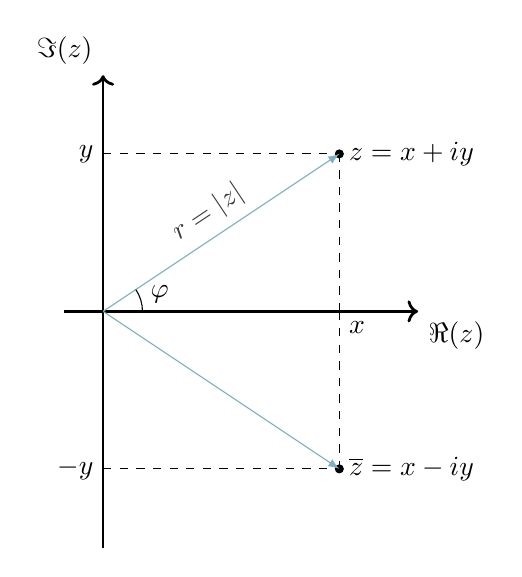
\begin{tikzpicture}
         % coords
         \coordinate (OR) at (0, 0);
         \coordinate (LX) at (-0.5, 0);
         \coordinate (RX) at (4, 0);
         \coordinate (TY) at (0, 3);
         \coordinate (BY) at (0, -3);

         % coordinate system
         \draw[->][line width=1.00pt] (LX) -- (RX) node[anchor=north west] {\(\Re(z)\)};
         \draw[->][line width=1.00pt] (BY) -- (TY) node[anchor=south east] {\(\Im(z)\)};

         \coordinate (z) at (3, 2);
         \coordinate (y) at (0, 2);
         \coordinate (x) at (3, 0);

         \draw[fill] (z) node[anchor=west]{\(z = x + iy\)} circle [radius=0.05];
         \draw[dashed] (x) node[anchor=north west]{\(x\)} -- (z);
         \draw[dashed] (y) node[anchor=east]{\(y\)} -- (z);
         \draw[-{latex}, blue] (OR) -- (z) node [midway, above, sloped, black] (TextNode) {\(r = |z|\)};
         \pic[draw, -, "\(\varphi\)", angle eccentricity=1.5] {angle=x--OR--z};

         \coordinate (conjz) at (3, -2);
         \coordinate (-y) at (0, -2);
         \draw[fill] (conjz) node[anchor=west]{\(\overline{z} = x - iy\)} circle [radius=0.05];
         \draw[dashed] (x) -- (conjz);
         \draw[dashed] (-y) node[anchor=east]{\(-y\)} -- (conjz);
         \draw[-{latex}, blue] (OR) -- (conjz);
      \end{tikzpicture}
   \end{figure}

   \begin{proposition}[\(\mathbb{C}\) is a Field]
      The set \(\mathbb{C}\) with the operations
      \[+: (x_1, y_1) + (x_2, y_2) = (x_1 + x_2, y_1 + y_2)\]
      \[\cdot: (x_1, y_1) \cdot (x_2, y_2) = (x_1x_2 - y_1y_2, x_1y_2 + x_2y_1)\]
      is a field.
   \end{proposition}
   \begin{proof}
      The additive neutral element is \((0, 0)\) and the inverse is \(-(x, y) = (-x, -y)\).

      The multiplicative neutral element is \((1, 0)\).
      The multiplicative inverse element is given through
      \[\frac{1}{x + iy} = \frac{x - iy}{(x+iy)(x-iy)} = \frac{x}{x^2 + y^2} - i\frac{y}{x^2 + y^2}\]
      \[(x, y)^{-1} := \left(\frac{x}{x^2 + y^2}, \frac{-y}{x^2 + y^2}\right)\]
   \end{proof}

   \begin{definition}[Complex Absolute Value]
      Given \(z = x + iy \in \mathbb{C}\)
      \[|z| := \sqrt{\overline{z}z} = \sqrt{x^2 + y^2}\]
   \end{definition}
   \begin{remark}
      The following calculation rules apply
      \[|z_1 \cdot z_2| = |z_1| \cdot |z_2|\]
      \[|z| = \iff z = 0\]
      \[|\Re(z)| \leq |z|\]
      \[|\Im(z)| \leq |z|\]
      \[|z_1 + z_2| \leq |z_1| + |z_2|\]
   \end{remark}

   % TODO: add polar coordinates

   \begin{theorem}[Fundamental Theorem of Algebra]
      Every polynomial
      \[p(x) = a_nx^n + a_{n-1}x^{n-1} + \ldots + a_1x + a_0\]
      with a rank \(n \geq 1\) and complex coefficients has at least one root (nullstelle) in \(\mathbb{C}\).
      Which means \(\exists w \in \mathbb{C}: p(w) = 0\)
   \end{theorem}

   \subsection{Vectorspaces \texorpdfstring{\(\mathbb{R}^m\)}{R(m)}}
   \begin{theorem}[\(\mathbb{R}^m\) is Vector Space]
      \(\forall m \in \mathbb{N} \setminus \{0\}: \mathbb{R}^m~\text{is a vector space.}\)
      \[\forall x, y \in \mathbb{R}^m: x + y = (x_1 + y_1, x_2 + y_2, \ldots, x_m + y_m)\]
      \[\forall \alpha \in \mathbb{R}, x \in \mathbb{R}^m: \alpha \cdot x = (\alpha \cdot x_1, \alpha \cdot x_2, \ldots, \alpha \cdot x_m)\]
   \end{theorem}

   \begin{definition}[Vector Length]
      \[\|\ldots\|: \mathbb{R}^m \to \mathbb{R} := x \mapsto \left(\sum_{j=1}^m x_j^2\right)^{\frac{1}{2}} = \sqrt{\sum_{j=1}^m x_j^2} = \sqrt{x_1^2 + x_2^2 + \ldots + x_m^2}\]
   \end{definition}
   \begin{remark}
      Also called the euclidean norm, fullfills the following properties
      \[\forall x \in \mathbb{R}^m: \|x\| \geq 0~\text{and}~\|x\| = 0~\text{if}~x = 0\]
      \[\forall \alpha \in \mathbb{R}, x \in \mathbb{R}^m: \|\alpha \cdot x\| = |\alpha| \cdot \|x\|\]
      \[\forall x, y \in \mathbb{R}^m: \|x + y\| \leq \|x\| + \|y\|\]
   \end{remark}
   \begin{proof}[Proof (\(\|x + y\| \leq \|x\| + \|y\|\))]
      Let \(x, y \in \mathbb{R}^m\), we define \(\langle x, y \rangle := \sum_{j=1}^m x_j \cdot y_j\)
      \[\|x\| = \sqrt{\langle x, x \rangle} \implies\]
      \[0 \leq \|x + \alpha y\|^2 = \langle x + \alpha y, x + \alpha y \rangle = \langle x, x \rangle + \alpha^2 \langle y, y \rangle + 2 \alpha \langle x, y\rangle \implies\]
      \[0 \leq \|x\|^2 + \alpha^2 \|y\|^2 + 2 \alpha \langle x, y \rangle\]
      Suppose \(y \neq 0\) and \(\alpha = \frac{\|x\|}{\|y\|}\)
      \[0 \leq 2 \|x\|^2 - 2\frac{\|x\|}{\|y\|} \langle x, y \rangle \implies \langle x, y \rangle \leq \|x\| \cdot \|y\|\]
   \end{proof}

   \section{Sequences}
   \begin{definition}[Sequence]
      A sequence \(a_n\) on a set \(X\) is an enumerated collection of objects.
      \[a_n = (a_n)_{n \in \mathbb{N}} := a_1, a_2, \ldots, a_n\]
      \[a: \mathbb{N} \to X \quad\text{where}\quad n \mapsto x\]
   \end{definition}
   \begin{remark}
      One can imagine a sequence as a list with a particular order.
      The number of elements (possibly infinite) is called the \textit{length} of the sequence.
   \end{remark}

   \subsection{Convergence}
   When we ask about the convergence of a sequence, we want to know what the last element looks like when we continue to infinity.

   \begin{definition}[Convergent Sequence]
      A sequence \(a_n\) over \(\mathbb{R}\) converges to \(a \in \mathbb{R}\) if
      \[\forall \varepsilon > 0~\exists n_0 \in \mathbb{N}: (\forall n > n_0: |a_n - a| < \varepsilon)\]
   \end{definition}
   \begin{remark}
      In other words, \(a_n\) converges to \(a\) if we can find the sequence length threshold \(n_0\) after which all \(a_n\) are closer to \(a\) than a chosen error margin \(\varepsilon\).
      This means that there comes a point \(n_0\) in the sequence after which all following elements are closer to \(a\) than an arbitrarily small \(\varepsilon\).
      It is important that \(\varepsilon\) can be chosen arbitrarily because only then we can write
      \[a_n \xrightarrow{n \to \infty} a \quad\text{or}\quad \lim_{n \to \infty} a_n = a\]

      Another way of stating the same becomes apparent when we note that
      \[a_n \to a \iff a_n - a \to 0 \iff |a_n - a| \to 0\]
      The absolute value \(|a_n - a|\) measures the distance between \(a_n\) and \(a\).
      Since \(\varepsilon\) can be arbitrarily small, \(a_n \to a\) means that this distance is smaller than the error margin if we choose \(n\) big enough.
      How big \(n\) must be is defined by \(n_0\) which depends on \(\epsilon\) which means that for a smaller \(\varepsilon\) \(n_0\) must be (typically) bigger.
      \[|a_n - a| < \epsilon \iff a - \varepsilon < a_n < a + \varepsilon \iff a_n \in (a - \varepsilon, a + \varepsilon)\]
   \end{remark}
   \begin{remark}
      When asked if a sequence \((a_n)_{n \in \mathbb{N}}\) converges we can answer with ''If you give me an \(\varepsilon\), I can give you an appropriate \(n_0\)``, since \(n_0\) depends on \(\varepsilon\).
   \end{remark}
   \begin{example}
      Let \(a_n = \frac{1}{n}\), then \(a_n \to 0\).

      Let \(\varepsilon > 0\) be arbitrary but fixed.
      According to \cref{cor:arch}
      \[\exists n_0 \in \mathbb{N}: \frac{1}{n_0} < \varepsilon \quad\text{it holds that}\quad \forall n > n_0: \frac{1}{n} < \frac{1}{n_0} \quad\text{and since}\quad \frac{1}{n_0} < \varepsilon \quad\text{follows}\]
      \[\forall \varepsilon > 0~\exists n_0: n > n_0 \implies \frac{1}{n} < \varepsilon\]

      \begin{center}
         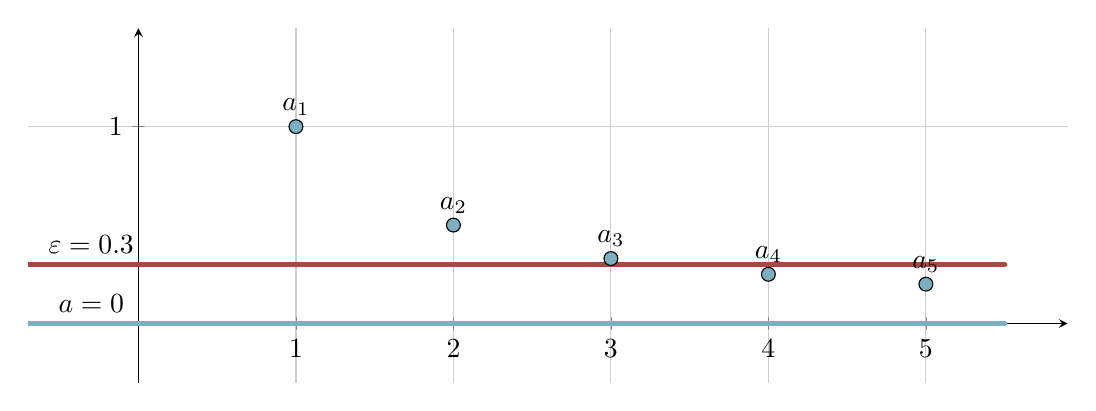
\begin{tikzpicture}[line cap=round, line join=round,>=triangle 45]
   \begin{axis}[
      x=2cm,y=2.5cm,
      axis lines=middle,
      ymajorgrids=true,
      xmajorgrids=true,
      xmin=-0.7,
      xmax=5.9,
      ymin=-0.3,
      ymax=1.5,
      xtick={0,1,...,5},
      ytick={0,1,...,2},
   ]

      \draw (-0.3,0.4) node {$\varepsilon = 0.3$};
      \draw [line width=2pt,color=red] (-1, 0.3) -- (5.5, 0.3);

      \draw (-0.3,0.1) node {$a = 0$};
      \draw [line width=2pt,color=blue] (-1, 0) -- (5.5, 0);

      \draw [fill=blue] (1,1) circle (2.5pt);
      \draw (1,1.1) node {$a_1$};

      \draw [fill=blue] (2,0.5) circle (2.5pt);
      \draw (2.,0.6) node {$a_2$};

      \draw [fill=blue] (3,0.33) circle (2.5pt);
      \draw (3.,0.43) node {$a_3$};

      \draw [fill=blue] (4,0.25) circle (2.5pt);
      \draw (4,0.35) node {$a_4$};

      \draw [fill=blue] (5,0.2) circle (2.5pt);
      \draw (5,0.3) node {$a_5$};
   \end{axis}
\end{tikzpicture}

      \end{center}
   \end{example}
   \begin{example}[Constant Sequence]
      Let \(a_n = c\), then \(a_n \to c\).

      Since \(a_n\) is constant the choice for \(n_0\) doesn't matter since \(\forall n_0 \in \mathbb{N}: a_{n_0} = c\), hence
      \[\forall \varepsilon > 0: |a_n - c| = 0 < \varepsilon\]
   \end{example}
   \begin{example}
      Let \(a_n = (-1)^n\).

      Since the values of \(a_n\) oscillate between 1 and -1, the sequence doesn't converge.
   \end{example}
   \begin{example}
      Let \(a_n = n\).

      Since the values of \(a_n\) only get bigger, the sequence doesn't converge.
   \end{example}
   \begin{example}
      \[\lim_{n \to \infty} \sqrt[n]{n} = \infty\]
   \end{example}
   \begin{example}
      \[\forall r \in \mathbb{R}_{>0}: \lim_{n \to \infty} \sqrt[n]{r} = 1\]
   \end{example}
   \begin{example}
      \[\forall s \in \mathbb{R}_{>0}: \lim_{n \to \infty} \sqrt[n]{n^s} = 1\]
   \end{example}
   \begin{example}
      \[\forall k \in \mathbb{N}, q \in \mathbb{C}: |q| < 1: \lim_{n \to \infty} n^k \cdot q^n = 0\]
   \end{example}
   \begin{example}
      \[\forall z \in \mathbb{C}: \lim_{n \to \infty} \left(1 + \frac{z}{n}\right)^n = e^z\]
   \end{example}
   \begin{example}
      \[\lim_{n \to \infty} \frac{n!}{n^n} = 0\]
   \end{example}

   \begin{proposition}[Unique Sequence Limit]\label{pro:unique_limit}
      Every sequence has only one limit.
   \end{proposition}

   \begin{definition}[Bounded Below Sequence]
      Given a sequence \(a_n \in \mathbb{R}\).
      \[\exists b \in \mathbb{R}: (\forall n \in \mathbb{N}: b \leq a_n)\]
   \end{definition}
   \begin{example}
      \(a_n = n\) is bounded below since \(\forall n \in \mathbb{N}: 0 \leq a_n\) but not bounded above.
   \end{example}

   \begin{definition}[Bounded Above Sequence]
      Given a sequence \(a_n \in \mathbb{R}\).
      \[\exists b \in \mathbb{R}: (\forall n \in \mathbb{N}: a_n \leq b)\]
   \end{definition}

   \begin{definition}[Bounded Sequence]
      A sequence \(a_n \in \mathbb{R}\) which is bounded above and below
      \[\exists b > 0 \in \mathbb{R}: (\forall n \in \mathbb{N}: |a_n| < b)\]
   \end{definition}
   \begin{example}
      \(a_n = \frac{1}{n}\) is bounded since \(\forall n \in \mathbb{N}: 0 \leq a_n \leq 1\).
   \end{example}
   \begin{example}
      \(a_n = (-1)^n\) is bounded since \(\forall n \in \mathbb{N}: -1 \leq a_n \leq 1\).
   \end{example}

   \begin{proposition}[Sequence Convergent \(\implies\) Bounded]\label{pro:convergent_bounded}
      Every convergent sequence is bounded.
   \end{proposition}
   \begin{remark}
      The contraposition: ''Every unbounded sequence diverges``, is often more usefull.
   \end{remark}

   \begin{lemma}[\(a_n \leq b_n \implies a \leq b\)]\label{lem:liman<limbn}
      Let \(a_n \to a\) and \(b_n \to b\) with \(\forall n \in \mathbb{N}: a_n \leq b_n\), then is \(a \leq b\).
   \end{lemma}
   \begin{remark}
      It is sufficient that \(\exists n_0 \in \mathbb{N}: n > n_0 \implies a_n \leq b_n\).
   \end{remark}

   \begin{center}
      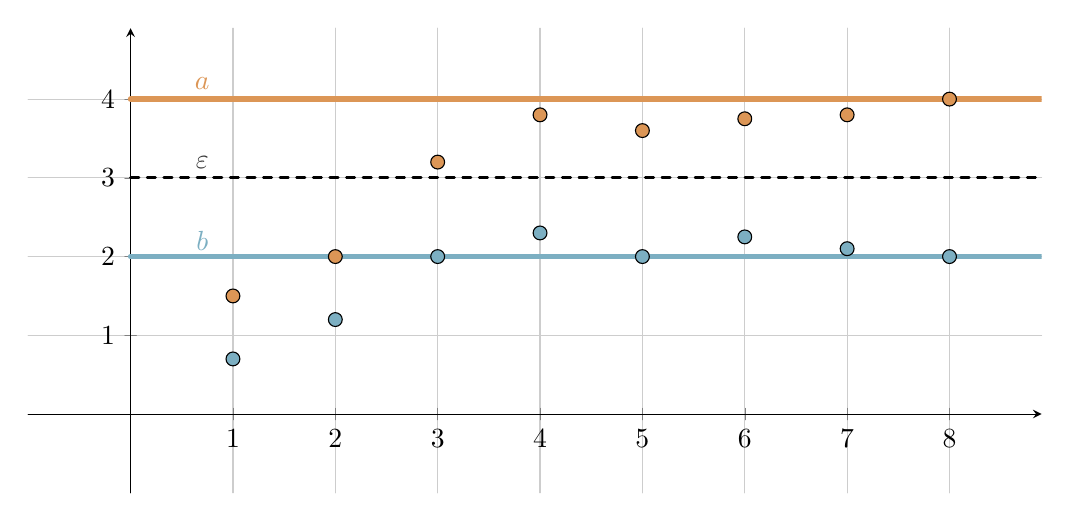
\begin{tikzpicture}[line cap=round,line join=round,>=triangle 45,x=1cm,y=1cm]
   \begin{axis}[
      x=1.3cm,y=1cm,
      axis lines=middle,
      ymajorgrids=true,
      xmajorgrids=true,
      xmin=-1,
      xmax=8.9,
      ymin=-1,
      ymax=4.9,
      xtick={0,1,...,9},
      ytick={0,1,...,5}]

   \draw[color=blue] (0.7, 2.2) node {\(b\)};
   \draw [line width=2pt,color=blue] (0, 2) -- (9, 2);

   \draw[color=orange] (0.7, 4.2) node {\(a\)};
   \draw [line width=2pt,color=orange] (0, 4) -- (9, 4);

   \draw[color=black] (0.7, 3.2) node {\(\varepsilon\)};
   \draw [line width=1pt,dashed] (0, 3) -- (9, 3);

   \draw [fill=blue] (1, 0.7) circle (2.5pt);
   \draw [fill=blue] (2, 1.2) circle (2.5pt);
   \draw [fill=blue] (3 ,2) circle (2.5pt);
   \draw [fill=blue] (4, 2.3) circle (2.5pt);
   \draw [fill=blue] (5, 2) circle (2.5pt);
   \draw [fill=blue] (6 ,2.25) circle (2.5pt);
   \draw [fill=blue] (7, 2.1) circle (2.5pt);
   \draw [fill=blue] (8, 2) circle (2.5pt);

   \draw [fill=orange] (1, 1.5) circle (2.5pt);
   \draw [fill=orange] (2, 2) circle (2.5pt);
   \draw [fill=orange] (3, 3.2) circle (2.5pt);
   \draw [fill=orange] (4, 3.8) circle (2.5pt);
   \draw [fill=orange] (5, 3.6) circle (2.5pt);
   \draw [fill=orange] (6, 3.75) circle (2.5pt);
   \draw [fill=orange] (7, 3.8) circle (2.5pt);
   \draw [fill=orange] (8, 4) circle (2.5pt);

   \end{axis}
\end{tikzpicture}

   \end{center}

   \begin{proposition}[Calculation Rules for Sequence Limits]\label{pro:R_field_operations}
      Let \(a_n \to a\) and \(b_n \to b\) be two sequences in \(\mathbb{R}\), then holds
      \begin{enumerate}[label=\roman*, align=Center]
         \item \[a_n + b_n \xrightarrow{n \to \infty} a + b\]
         \item \[a_n - b_n \xrightarrow{n \to \infty} a - b\]
         \item \[a_n \cdot b_n \xrightarrow{n \to \infty} a \cdot b\]
         \item For \(b \neq 0\) and \(\forall n \in \mathbb{N}: b_n \neq 0\)
            \[\frac{a_n}{b_n} \xrightarrow{n \to \infty} \frac{a}{b}\]
         \item If \(\forall n \in \mathbb{N}: a_n \geq 0\)
            \[p \in \mathbb{Z}, q \in \mathbb{Z} \setminus \{0\}: a_n^{\frac{p}{q}} \to a^{\frac{p}{q}}\]
      \end{enumerate}
   \end{proposition}
   \begin{example}
      \[a_n = \frac{n^2 + 3n + 5}{3n^2 + 8n + 1}\]
      Since \(n^2\) dominates we can regard it as \(a_n = \frac{n^2}{3n^2}\) and can easily see that \(\lim_{n \to \infty} a_n = \frac{1}{3}\).
      But we can also regard this sequence through the proposition, when we divide the term by \(n^2\)
      \[a_n = \frac{1 + \frac{3}{n} + \frac{5}{n^2}}{3 + \frac{8}{n} + \frac{1}{n^2}}\]
      we see that \(\frac{3}{n} + \frac{5}{n^2}  \to 0 + 0\) and \(\frac{8}{n} + \frac{1}{n^2} \to 0 + 0\) so
      \[a_n = \frac{1 + 0 + 0}{3 + 0 + 0} = \frac{1}{3}\]
   \end{example}
   \begin{example}
      \[a_n = n \cdot \left(\sqrt{1 + \frac{1}{n}} - 1\right)\]
      We can't use the proposition since the factor \(n\) doesn't converge so we rewrite the sequence.
      \[n \cdot \left(\sqrt{1 + \frac{1}{n}} - 1\right) = n \cdot \frac{\left(\sqrt{1 + \frac{1}{n}} - 1\right) \cdot \left(\sqrt{1 + \frac{1}{n}} + 1\right)}{\left(\sqrt{1 + \frac{1}{n}} + 1\right)} = n \cdot \frac{\frac{1}{n}}{\left(\sqrt{1 + \frac{1}{n}} + 1\right)}\]
      Since \(\frac{1}{n} \to 0\) we have \(\frac{1}{\sqrt{1 + 0} + 1}\) and we see that \(a_n \to \frac{1}{2}\).
   \end{example}

   \begin{definition}[Zero Sequence]
      A sequence \((a_n)_{n \in \mathbb{N}}\) which converges to 0 i.e. \(a_n \xrightarrow{n \to \infty} 0\).
   \end{definition}

   \begin{lemma}\label{lem:seq_converge_0}
      Let \((a_n)_{n \in \mathbb{N}}\) be a zero sequence and \(b_n\) a bounded sequence.
      \[a_n \cdot b_n \to 0\]
   \end{lemma}
   \begin{example}
      Let \(a_n = (-1)^n \cdot \frac{1}{n}\).
      Since \((-1)^n\) is bounded and \(\frac{1}{n} \to 0\) follows \(a_n \to 0\).
   \end{example}

   \begin{proposition}[Sandwich Sequence]\label{pro:sandwich_seq}
      For \(n \in \mathbb{N}\) let \((a_n)\), \((b_n)\) and \((c_n)\) be sequences with
      \[\forall n > n_0: a_n \leq b_n \leq c_n \quad\text{and}\quad \lim_{n \to \infty} a_n = \lim_{n \to \infty} c_n = d\]
      then is
      \[\lim_{n \to \infty} b_n = d\]
   \end{proposition}
   \begin{example}
      We want to prove \(\lim_{n \to \infty} \frac{\sin(n)}{n} = 0\).
      We know that \(-1 \leq \sin(x) \leq 1 \implies -\frac{1}{n} \leq \frac{\sin(x)}{n} \leq \frac{1}{n}\).
      So we found \(a_n = -\frac{1}{n}\), \(c_n = \frac{1}{n}\) for \(b_n = \frac{\sin(n)}{n}\) such that
      \[\forall n \in \mathbb{N}: a_n \leq b_n \leq c_n \quad\text{and}\quad \lim_{n \to \infty} a_n = \lim_{n \to \infty} c_n = 0\]
      hence \(\lim_{n \to \infty} \frac{\sin(n)}{n} = 0\).
   \end{example}

   \begin{lemma}[\(n^pq^n \to 0\)]\label{lem:exponent_converge_0}
      Let \(p \in \mathbb{N}\) and \(|q| < 1\), then \(n^p \cdot q^n \to 0\).
   \end{lemma}
   \begin{remark}
      This means that \(q^n \to 0\) - another important example of a sequence - converges faster than any other power of \(n\).
   \end{remark}

   \subsection{Monotone Sequences}
   \begin{definition}[Increasing Sequence]
      Given a sequence \((a_n)_{n \in \mathbb{N}} \subset \mathbb{R}\).
      \[\forall n \in \mathbb{N}: a_n \leq a_{n+1}\]
   \end{definition}
   \begin{remark}
      If \(m > n \implies a_m > a_n\), \(a_n\) is \textit{strictly} increasing.
   \end{remark}

   \begin{definition}[Decreasing Sequence]
      Given a sequence \((a_n)_{n \in \mathbb{N}} \subset \mathbb{R}\).
      \[\forall n \in \mathbb{N}: a_n \geq a_{n+1}\]
   \end{definition}
   \begin{remark}
      If \(m < n \implies a_m > a_n\), \(a_n\) is \textit{strictly} decreasing.
   \end{remark}

   \begin{remark}[Show Monotonic Behaviour]
      We have 4 equivalent options
      \begin{enumerate}
         \item \(a_{n+1} = \ldots \geq a_n\)
         \item \(\frac{a_{n+1}}{a_n} = \ldots \geq 1\)
         \item \(a_{n+1} - a_n = \ldots \geq 0\)
         \item For a recursive sequence we can use induction.
      \end{enumerate}
   \end{remark}

   \begin{proposition}[Monotone \& Bounded \(\implies\) Convergent]\label{pro:convergent_monotone_sequence_bounded}
      Let \(a_n \in \mathbb{R}\) be an increasing sequence and \(b_n \in \mathbb{R}\) a decreasing sequence.
      \[a_n~\text{convergent} \iff a_n~\text{bounded above} \quad\text{and}\quad b_n~\text{convergent} \iff b_n~\text{bounded below}\]
   \end{proposition}
   \begin{example}
      Let \(a_0 := a \geq 1\) and \(a_{n+1} := \frac{1}{2} \left(a_n + \frac{a}{a_n}\right)\).
      We want to prove that \(\lim_{n \to \infty} a_n = \sqrt{a}\).

      First we prove that \(a_n\) is decreasing.
      \[a_{n+1} = \frac{1}{2} \left(a_n + \frac{a}{a_n}\right) = \frac{a_n}{2} \left(1 + \frac{a}{a_n^2}\right) \overset{a_n^2 \geq a}{\leq} \frac{a_n}{2} \left(1 + \frac{a}{a}\right) = a_n\]

      Now we show that \(a_n\) is bounded below by induction over \(n\)

      \textit{IB:} \(n = 0 \implies a_0 = a \geq \sqrt{a}\) holds since \(a \geq 1\).

      \textit{IH:} For some \(n \in \mathbb{N}\) holds \(a_n \geq \sqrt{a}\).

      \textit{IS:} Assume IH holds.
      \begin{equation*}
         \begin{split}
            a_{n+1} \geq \sqrt{a} & \iff \frac{1}{2} \left(a_n + \frac{a}{a_n}\right) \geq \sqrt{a} \iff a_n + \frac{a}{a_n} \geq 2 \sqrt{a}\\
                                  & \iff a_n - 2\sqrt{a} \geq - \frac{a}{a_n} \iff a_n(a_n - 2\sqrt{a}) \geq -a
         \end{split}
      \end{equation*}
      but
      \[a_n(a_n - 2 \sqrt{a}) \overset{\text{IH}}{\geq} \sqrt{a}(\sqrt{a} - 2 \sqrt{a}) = -a\]
      So according to the induction axiom and IB, IH, IS follows that \(a_n\) is bounded below \(\forall n \in \mathbb{N}\).
   \end{example}

   \subsection{Limessuperior \& Limesinferior}
   Let \(a_n\) be a bounded sequence: \(\forall n \in \mathbb{N}: |a_n| \leq b\).
   We define
   \[\overline{a}_n := \sup\{a_j \mid j \geq n\} \quad\text{and}\quad \underline{a}_n := \inf\{a_j \mid j \geq n\}\]
   Since \(a_n\) is bounded holds \(\forall \in \mathbb{N}: -b \leq \underline{a}_n \leq \overline{a}_n \leq b\) which means that they both are bounded.
   Furthermore follows from their definitions that \(\overline{a}_n\) is increasing and \(\underline{a}_n\) is decreasing.
   Hence they are convergent according to \cref{pro:convergent_monotone_sequence_bounded}.

   % TODO: describe/visualize
   \begin{definition}[Limessuperior]
      Given a bounded sequence \(a_n \in \mathbb{R}\).
      \[\limsup_{n \to \infty}(a_n) := \lim_{n \to \infty} \overline{a}_n\]
   \end{definition}
   \begin{definition}[Limesinferior]
      Given a bounded sequence \(a_n \in \mathbb{R}\).
      \[\liminf_{n \to \infty}(a_n) := \lim_{n \to \infty} \underline{a}_n\]
   \end{definition}
   \begin{remark}
      \(\liminf\) is the smallest clusterpoint and \(\limsup\) the largest.
   \end{remark}
   \begin{example}
      Let \(a_n := (-1)^n \left(1 + \frac{1}{n}\right)\).
      We have
      \[\sup a_n = a_2 = \frac{3}{2} \quad\text{and}\quad \inf a_n = a_1 = -2\]
      \[\limsup_{n \to \infty} a_n = 1 \quad\text{and}\quad \liminf_{n \to \infty} a_n = -1\]
   \end{example}
   \begin{example}
      Let \(a_n = \frac{1}{n}\), then are
      \[\overline{a}_n = \sup\left\{\frac{1}{j}~\middle|~j \geq n\right\} = \frac{1}{n} \quad\text{and}\quad \underline{a}_n = \inf\left\{\frac{1}{j}~\middle|~j \geq n\right\} = 0\]
      \[\begin{drcases}
         \overline{a}_n \to 0\\
         \underline{a}_n \to 0
      \end{drcases} \implies \liminf_{n \to \infty}(a_n) = 0 = \limsup_{n \to \infty}(a_n) \implies a_n~\text{converges}\]
   \end{example}
   \begin{example}
      Let \(a_n = (-1)^n\), then are 
      \[\overline{a}_n = \sup\{(-1)^j \mid j \geq n\} = 1 \quad\text{and}\quad \underline{a}_n = \inf\{(-1)^j \mid j \geq n\} = -1\]
      \[\limsup_{n \to \infty}(a_n) = 1 \quad\text{and}\quad \liminf_{n \to \infty}(a_n) = -1 \quad\text{hence}\quad a_n~\text{doesn't converge}\]
   \end{example}

   \begin{theorem}[\(\liminf = \limsup \iff a_n\) convergent]\label{thm:limsup_inf_rules}
      Let \(a_n\) be a bounded sequence.
      \begin{equation}\label{eq:inf<sup}
         \liminf_{n \to \infty}(a_n) \leq \limsup_{n \to \infty}(a_n)
      \end{equation}
      \begin{equation}\label{eq:liminf=limsup}
         a_n~\text{converges} \iff \liminf_{n \to \infty}(a_n) = \limsup_{n \to \infty}(a_n)
      \end{equation}
      \begin{equation}\label{eq:liman=limsup=liminf}
         a_n~\text{converges} \iff \lim_{n \to \infty}(a_n) = \liminf_{n \to \infty}(a_n) = \limsup_{n \to \infty}(a_n)
      \end{equation}
   \end{theorem}

   \begin{definition}[For Almost All]
      A predicate \(A(n)\) holds for \textit{almost all} \(n \in \mathbb{N}\) if
      \[\big|\{n \in \mathbb{N} \mid \neg A(n)\}\big| < \infty\]
   \end{definition}
   \begin{remark}
      In other words, \(A(n)\) holds for almost all \(n\) if it is wrong for only finitely many.
      With this definition we can formulate convergence differently
      \[a_n \to a \iff \forall \varepsilon > 0: |a_n - a| < \varepsilon~\text{for almost all}~n \in \mathbb{N}\]
   \end{remark}

   \begin{theorem}\label{thm:bounded_seq}
      Let \(a_n\) be a bounded sequence, then is \(\overline{a} = \limsup_{n \to \infty}(a_n)\) iff
      \[\forall \varepsilon > 0: a_n \leq \overline{a} + \varepsilon~\text{for almost all}~n \in \mathbb{N} \quad\text{and}\quad \forall \varepsilon > 0: a_n > \overline{a} - \varepsilon~\text{for infinite}~n \in \mathbb{N}\]
   \end{theorem}
   \begin{remark}
      \[a_n \to a \iff \forall \varepsilon > 0: \begin{cases} a_n < a + \varepsilon~\text{for almost all}~n \in \mathbb{N}\\ a_n > a - \varepsilon~\text{for almost all}~n \in \mathbb{N} \end{cases}\]
      \[\limsup_{n \to \infty}(a_n) = a \iff \forall \varepsilon > 0: \begin{cases} a_n < a + \varepsilon~\text{for almost all}~n \in \mathbb{N}\\ a_n > a - \varepsilon~\text{for infinite}~n \in \mathbb{N} \end{cases}\]
   \end{remark}

   \subsection{Cluster Point \& Subsequence}
   \begin{definition}[Cluster Point of a Sequence]
      Given a sequence \(a_n \in \mathbb{R}\).

      \(b \in \mathbb{R}\) is a cluster point of \(a_n\) if
      \[\forall \varepsilon > 0: |a_n - b| < \varepsilon~\text{for infinite}~n \in \mathbb{N}\]
   \end{definition}
   \begin{remark}
      Cluster points are similar to the limit of a sequence where
      \[\lim_{n \to \infty} a_n = b\]
      \[\forall \varepsilon > 0: |a_n - b| < \varepsilon~\text{for almost all}~n \in \mathbb{N}\]
   \end{remark}
   \begin{example}
      \(a_n = (-1)^n\) doesn't converge but it has the cluster points \(\pm 1\).
   \end{example}
   \begin{example}
      \(a_n = \frac{1}{n}\) has the cluster point \(0 = \lim_{n \to \infty} a_n\).
   \end{example}

   \begin{corollary}\label{cor:bounded_subsequence_cluster_point}
      Every bounded sequence has at least one cluster point and converges iff it has only one clusterpoint.
   \end{corollary}
   \begin{proof}
      Left out.
   \end{proof}
   \begin{remark}
      It follows from \cref{thm:bounded_seq} that for every bounded sequence \(\limsup, \liminf\) are clusterpoints.
      Furthermore are cluster points the limits of subsequences.
   \end{remark}

   \begin{definition}[Subsequence]
      A subsequence of \(a_n\) is
      \[a_{n_j} = a_{n_1}, a_{n_2}, \ldots \quad\text{a map}\quad a \circ \phi: \mathbb{N} \to \mathbb{R}\]
      where \(\phi: \mathbb{N} \to \mathbb{N}\) must be strictly increasing: \(n_1 < n_2 \implies \phi(n_1) < \phi(n_2)\)
   \end{definition}
   \begin{example}
      Let \(a_n = n = 1, 2, 3, \ldots\).
      \[\begin{drcases}
            a: \mathbb{N} \to X \quad\text{where}\quad n \mapsto n \\
            \phi: \mathbb{N} \to \mathbb{N} \quad\text{where}\quad n \mapsto 2n
      \end{drcases} a \circ \phi: \mathbb{N} \to \mathbb{N} \to X\]
      \[a_1 = a(1) = 1 \qquad a_2 = a(2) = 2 \qquad a_3 = a(3) = 3\]
      \[a_{n_1} = a(\phi(1)) = a(2) = 2 \qquad a_{n_2} = a(\phi(2)) = a(4) = 4 \qquad a_{n_3} = a(\phi(3)) = a(6) = 6\]
      From the definition of \(\phi\) is clear how the indices of the subsequence come into place.
      This means we can write the created subsequence in terms of the index of \(a_n\) (without the subindices \(n_j\)) which is \(a_{2n} = a_2, a_4, a_6, \ldots = 2, 4, 6, \ldots\).
   \end{example}

   \begin{proposition}[Subsequence of Convergent Sequence]\label{pro:subseq_conv}
      Let \(a_n \to a\) be a sequence, then converges every subsequence of \(a_n\) also to \(a\).
   \end{proposition}
   \begin{remark}
      Even if \(a_n\) is divergent there might exist convergent subsequences.
      For example \(a_n = (-1)^n\), \(a_{2n} \to 1\) and \(a_{2n+1} \to -1\).
   \end{remark}

   \begin{proposition}\label{pro:subseq_converges_cluster_point}
      Let \(a_n \in \mathbb{R}\) be a sequence.
      \[b~\text{is a cluster point of}~a_n \iff \exists n_j: \mathbb{N} \to \mathbb{N}: a_{n_j} \to b\]
   \end{proposition}

   \begin{corollary}[Bolzano-Weierstrasse]\label{cor:bolzano_weierstrasse}
      Every bounded sequence on \(\mathbb{R}\) has a convergent subsequence.
   \end{corollary}
   \begin{example}
      Let \(a_n = (-1)^n\).
      \(a_n\) is bounded above and below and thus has convergent subsequence
      \[\lim_{n \to \infty} a_{2n} = 1 \quad\text{and}\quad \lim_{n \to \infty} a_{2n-1}\]
   \end{example}

   \subsection{Cauchy-Sequences}
   \begin{definition}[Cauchy Condition]\label{def:cauchy_condition}
      Let \(a_n \to a\) be a sequence on \(\mathbb{R}\) and \(\varepsilon > 0\).
      \[\exists n_0 \in \mathbb{N}: n > n_0 \implies |a_n -a| < \frac{\varepsilon}{2}\]
   \end{definition}
   \begin{remark}
      We can rewrite this condition for \(n, m \in \mathbb{N}: n, m > n_0\)
      \[|a_n - a_m| = |a_n - a + a_m - a| \leq |a_n - a| + |a_m - a| < \varepsilon\]
   \end{remark}

   \begin{definition}[Cauchy Sequence]
      Given a sequence \(a_n\) where
      \[\forall \varepsilon > 0~\exists n_0 \in \mathbb{N}: (\forall n, m > n_0: |a_n - a_m| < \varepsilon)\]
   \end{definition}
   \begin{remark}
      In other words, it is a sequence whose elements become arbitrarily close to each other as the sequence progresses.
      More precisely, given any small positive distance, all but a finite number of elements of the sequence are less than that given distance from each other.
   \end{remark}

   \begin{center}
      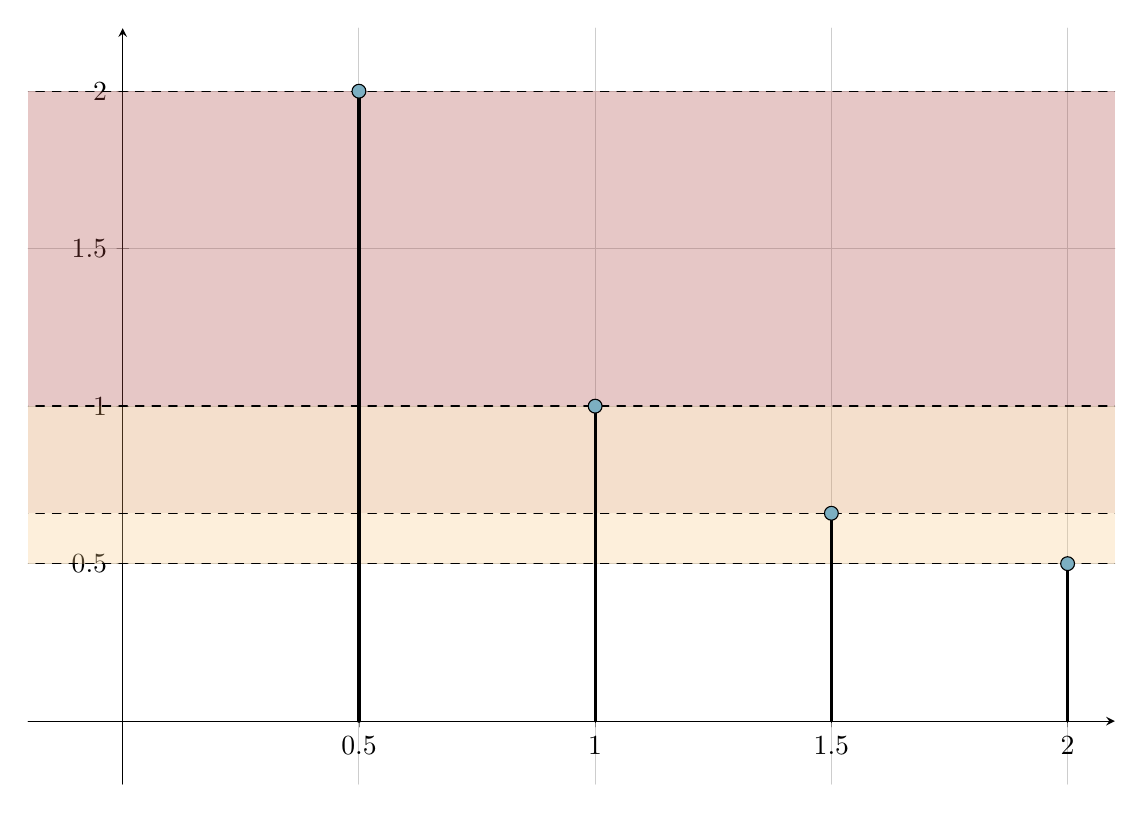
\begin{tikzpicture}[line cap=round,line join=round,>=triangle 45,x=1cm,y=1cm]
   \begin{axis}[
      x=6cm, y=4cm,
      axis lines=middle,
      ymajorgrids=true,
      xmajorgrids=true,
      xmin=-0.2, xmax=2.1,
      ymin=-0.2, ymax=2.2,
      xtick={0,0.5,...,2.2},
      ytick={0,0.5,...,2},]

      \fill[line width=2pt,color=red,fill=red,fill opacity=0.3] (-0.5,2) -- (2.5,2) -- (2.5,1) -- (-0.5,1) -- cycle;

      \fill[line width=2pt,color=orange,fill=orange,fill opacity=0.3] (-0.5,1) -- (2.5,1) -- (2.5, 0.66) -- (-0.5, 0.66) -- cycle;

      \fill[line width=2pt,color=yellow,fill=yellow,fill opacity=0.3] (-0.5, 0.66) -- (2.5, 0.66) -- (2.5,0.5) -- (-0.5,0.5) -- cycle;

      \draw[line width=0.5pt,dashed] (-0.5, 2) -- (2.5, 2);
      \draw[line width=0.5pt,dashed] (-0.5, 1) -- (2.5, 1);
      \draw[line width=0.5pt,dashed] (-0.5, 0.66) -- (2.5, 0.66);
      \draw[line width=0.5pt,dashed] (-0.5, 0.5) -- (2.5, 0.5);


      \draw [line width=1.2pt] (0.5,2)-- (0.5,0);
      \draw [line width=1.2pt] (1,1)-- (1,0);
      \draw [line width=1.2pt] (1.5,0.66)-- (1.5,0);
      \draw [line width=1.2pt] (2,0.5)-- (2,0);

      \draw [fill=blue] (0.5, 2) circle (2.5pt);
      \draw [fill=blue] (1, 1) circle (2.5pt);
      \draw [fill=blue] (1.5, 0.66) circle (2.5pt);
      \draw [fill=blue] (2, 0.5) circle (2.5pt);
   \end{axis}
\end{tikzpicture}

   \end{center}

   \begin{theorem}[Cauchy Criterion for Sequences]\label{thm:cauchy_crit_seq}
      Let \(a_n \in \mathbb{R}\) be a sequence.
      \[a_n~\text{convergent} \iff a_n~\text{cauchy sequence}\]
   \end{theorem}
   \begin{remark}
      Only holds on order complete fields.
      So for example \(a_n\) on \(\mathbb{R}^m\) converges iff
      \[\forall \varepsilon > 0: \exists n_0 = n_0(\varepsilon): \|a_n - a_m\| < \varepsilon, \forall n > n_0\]
   \end{remark}

   \subsection{Improper Limits}
   Many sequences such as \(a_n = n\) do not converge since they diverge into \(\infty\).
   We would need \(-\infty\) and \(+\infty\) to be limits to keep working with those sequences.
   Therefor we regard these sequences as convergent in the extended real numbers.

   \begin{definition}[Extended Real Numbers]
      \[\overline{\mathbb{R}} := \mathbb{R} \cup \{-\infty, +\infty\}\]
      \[\forall a \in \overline{\mathbb{R}}: -\infty < a < \infty\]
   \end{definition}
   \begin{remark}
      \(\overline{\mathbb{R}}\) is not a field.
   \end{remark}

   \begin{definition}[Improper Limit of Sequences]
      Given a sequence \(a_n \in \overline{\mathbb{R}}\).
      \[a_n~\text{diverges to}~+\infty~\text{if}~\forall M \in \mathbb{R}~\exists n_0 \in \mathbb{N}: (\forall n > n_0: a_n \geq M)\]
      \[a_n~\text{diverges to}~-\infty~\text{if}~\forall M \in \mathbb{R}~\exists n_0 \in \mathbb{N}: (\forall n > n_0: a_n \leq M)\]
   \end{definition}
   \begin{remark}[Features of Improper Limits]
      A monotone sequence in \(\overline{\mathbb{R}}\) has always a limit.

      The limes superior and inferior exist always and \(a_n\) converges in the proper or improper way iff \(\limsup_{n \to \infty}(a_n) = \liminf_{n \to \infty}(a_n)\)

      Every sequence in \(\overline{\mathbb{R}}\) has at least one proper or improper cluster point.
      For example
      \[a_n = \begin{cases} n~\text{even}: & \frac{1}{n}\\ n~\text{uneven}: & n\end{cases}\]
      has two cluster points, 0 and \(\infty\) and hence doesn't converge.

      \[a_n \to \infty \land b_n \to b \implies a_n + b_n \to \infty\]
      \[a_n \to -\infty \land b_n \to b \implies a_n + b_n \to -\infty\]
      \[a_n \to -\infty \land b_n \to +\infty \implies \text{no general rule}\]

      \[a_n \to \infty \land b_n \to b\]
      \[b > 0 \implies a_n \cdot b_n \to \infty\]
      \[b < 0 \implies  a_n \cdot b_n \to -\infty\]
      \[b = 0 \implies \text{no general rule}\]

      \[a_n \to \pm\infty \implies \frac{1}{a_n} \to 0\]

      \[\forall M \in \mathbb{R}: a_n > M~\text{for infinite}~n \in \mathbb{N} \implies +\infty~\text{is a cluster point of}~a_n\]
      \[\forall M \in \mathbb{R}: a_n < M~\text{for infinite}~n \in \mathbb{N} \implies -\infty~\text{is a cluster point of}~a_n\]
   \end{remark}

   \begin{example}
      \(\lim_{n \to \infty} \log(n) = \infty\).

      Let \(M \in \mathbb{R}\) be arbitrary but fixed.
      According to the axiom of archimedes \(\exists n_0 \in \mathbb{N}: n_0 \geq \lceil e^M \rceil\).
      Let \(n > n_0\) then holds that \(\log(n) > \log(n_0) \geq M\).
   \end{example}

   \section{Series}
   \subsection{Definition \& Basic Properties}
   \begin{definition}[Series]
      Given a sequence \((a_n)_{n \in \mathbb{N}}\).
      \[\sum_{n=0}^{\infty} a_n = a_0 + a_1 + \ldots + a_n\]
   \end{definition}

   \begin{definition}[Partial Sum]
      Given a series \(s = \sum_{n = 0}^{\infty} a_n\) its \textit{k}th partial sum is
      \[s_k := \sum_{n = 0}^{k} a_n = a_0 + \ldots + a_k\]
   \end{definition}
   \begin{remark}
      We say \((s_k)_{k \in \mathbb{N}} = \sum_{n=0}^k a_n\) is the \textit{sequence of partial sums}.
   \end{remark}

   \begin{definition}[Convergence of Series]\label{def:series_convergence}
      A series converges if the sequence of its partial sums has a limit.
      \[\sum_{n = 0}^{\infty} a_n := \lim_{k \to \infty} s_k = \lim_{k \to \infty} \sum_{n = 0}^k a_n\]
   \end{definition}
   \begin{remark}
      The value of this limit, if it exists, is then the \textit{value of the series}.
      If \(s_k \to \pm\infty\) we say the series \textit{diverges}.
      If it neither converges nor diverges we say the series \textit{doesn't exist}.
      Whether a series converges only depends on the asymptotic behavior of \(a_n\).
      \[\sum_{n = 0}^\infty a_n~\text{converges} \iff \sum_{n = m}^\infty a_n~\text{converges}\]
   \end{remark}
   \begin{example}
      The following series diverges to \(\infty\).
      \[\sum_{n = 0}^\infty n = \lim_{k \to \infty} \sum_{n = 0}^k n = \lim_{n \to \infty} \frac{n(n + 1)}{2}\]
   \end{example}
   \begin{example}
      The following series does not exist.
      \[\sum_{n = 0}^\infty (-1)^n\]
      \[s_k = \begin{cases}
            n~\text{uneven} & (-1)^k \cdot \frac{n + 1}{2}\\
            n~\text{even} & \frac{n}{2}
         \end{cases}
      \]
   \end{example}
   \begin{example}[Geometric Series]
      Let \(q \in \mathbb{R}\)
      \[q = 1 \implies \sum_{n = 0}^\infty q^n = \infty \qquad\qquad q \neq 1 \implies \sum_{n = 0}^\infty q^n = \frac{1-q^{n+1}}{1-q}\]
      \[|q| > 1 \implies \sum_{n = 0}^\infty q^n = \frac{1}{1-q} \qquad\qquad q \leq -1 \implies \sum_{n = 0}^\infty q^n~\text{doesn't exist}\]
      This holds because
      \[s_k = \sum_{n = 0}^k q^n = 1 + q + q^2 + \ldots + q^n\]
      where we see that
      \[s_k \cdot (1 - q) = 1 + (q - q) + \ldots + (q^n - q^n) - q^{n+1} = 1-q^{n+1}\]
      hence
      \[s_k = \frac{1 - q^{n+1}}{1 - q}\]
   \end{example}
   \begin{example}[Harmonic Series]
      \[\sum_{n = 1}^\infty \frac{1}{n}\]
      \[s_k = \sum_{n = 1}^k \frac{1}{n} = 1 + \frac{1}{2} + \ldots + \frac{1}{n}\]
      \[s_{2k} - s_k = \frac{1}{n+1} + \frac{1}{n + 2} + \ldots + \frac{1}{2n} \geq n \cdot \frac{1}{2n} = \frac{1}{2}\]
      No matter how big we choose \(k\), \(s_{2k} - s_k \geq \frac{1}{2}\) will always hold.
      This means \(s_k\) can't be a cauchy sequence, since the distances of the series elements is not getting smaller.
      This means the series diverges.
      \[\sum_{n = 0}^\infty \frac{1}{n} = \infty\]
      To put it differently: \(\frac{1}{n}\) does not approach 0 fast enough so that the whole series would converge to 0.
      The sum ''overtakes`` the convergence behaviour of \(\frac{1}{n}\) which is why it diverges to \(\infty\).
   \end{example}
   \begin{example}[Telescoping Series]
      \[\sum_{n=0}^\infty (a_{n+1} - a_n) = -a_0 + \lim_{n \to \infty} a_n\]
   \end{example}
   \begin{example}[Eulers Number]
      \[\sum_{n = 0}^\infty \frac{1}{n!} = e\]
   \end{example}

   \begin{proposition}[Series Calculation Rules]\label{pro:series_calc_rules}
      Let \(\alpha \in \mathbb{R}\) and let \(\sum_{n=0}^\infty a_n\), \(\sum_{n=0}^\infty b_n\) be converget series, then is
      \[\sum_{n=0}^\infty (a_n + b_n)~\text{convergent and} \qquad \sum_{n = 0}^\infty (a_n + b_n) = \sum_{n = 0}^\infty a_n + \sum_{n = 0}^\infty b_n\]
      \[\sum_{n = 0}^\infty \alpha \cdot a_n~\text{convergent and} \qquad \sum_{n = 0}^\infty \alpha \cdot a_n = \alpha \cdot \sum_{n=0}^\infty a_n\]
   \end{proposition}
   \begin{remark}
      \[\sum_{n = 0}^\infty \frac{1}{a_n}~\text{diverges}\]
   \end{remark}
   \begin{proof}
      Use \cref{pro:R_field_operations} on the series.
   \end{proof}

   \subsection{Convergence Criteria \& Applications}
   \begin{proposition}[Term Test]\label{pro:series_sequence_converge}
      Let \((a_n)_{n \in \mathbb{N}}\) be a sequence.
      \[\sum_{n = 0}^\infty a_n~\text{converges} \implies a_n \to 0\]
   \end{proposition}
   \begin{remark}
      This is mostly used in a contraposition to show divergence.
      Hence if \(a_n\) is not a zero sequence then follows that the series diverges.
   \end{remark}
   \begin{remark}
      A zero sequence is necessary but not sufficient for the convergence of the series.
      The harmonic series diverges even though \(\frac{1}{n} \to 0\).
   \end{remark}

   \begin{theorem}[Monotonicity Criterion]\label{thm:convergence=bounded}
      Let \((a_n)_{n \in \mathbb{N}}\) be a sequence with \(\forall n \in \mathbb{N}: 0 \leq a_n\).
      \[\sum_{n = 0}^\infty a_n~\text{converges} \iff (s_k)_{k \in \mathbb{N}}~\text{is bounded}\]
   \end{theorem}

   \begin{theorem}[Cauchy Criterion for Series]\label{thm:cauchy_crit_ser}
      \[\sum_{n=0}^\infty a_n\text{converges} \iff \forall \varepsilon > 0: \exists n_0 \in \mathbb{N}:  (\forall m > n > n_0: \left| \sum_{i = n + 1}^m a_i \right| < \varepsilon)\]
   \end{theorem}

   \begin{definition}[Absolute Convergent Series]
      Given a sequence \((a_n)_{n \in \mathbb{N}}\).
      \[\sum_{n=0}^\infty a_n~\text{is absolute convergent} :\iff \sum_{n=0}^\infty |a_n|~\text{converges}\]
   \end{definition}
   \begin{remark}
      So if a series is not absolute convergent, then is
      \[\sum_{n=0}^\infty |a_n| = \infty\]
   \end{remark}

   \begin{proposition}[Absolute Convergence Test]\label{pro:abs_conv_imply_conv}
      Every absolute convergent series is convergent.
   \end{proposition}
   \begin{remark}
      Absolute convergence is sufficient for convergence but not necessary.
   \end{remark}

   \begin{proposition}[Generalized Triangle Inequality]\label{pro:gener_triang_ineq}
      \[\left|\sum_{n = 0}^\infty a_n \right| \leq \sum_{n = 0}^\infty |a_n|\]
   \end{proposition}

   \begin{proposition}[(Direct) Comparison Test]\label{pro:comparison_test}
      Let \((a_n)_{n \in \mathbb{N}}\) where \(\forall n \in \mathbb{N}: 0 \leq a_n\) and \((b_n)_{n \in \mathbb{N}}\) where for almost all \(n \in \mathbb{N}: b_n \leq a_n\), then is
      \[\sum_{n=0}^\infty a_n~\text{convergent} \implies \sum_{n=0}^\infty b_n~\text{convergent}\]
      \[\sum_{n=0}^\infty b_n~\text{divergent} \implies \sum_{n=0}^\infty a_n~\text{divergent}\]
   \end{proposition}
   \begin{remark}
      This proposition provides a way of deducing the convergence or divergence by comparing the given series to one whose convergence properties are known.
      Typical series to use for comparison are the geometric and harmonic series.
   \end{remark}
   \begin{example}
      The series
      \[\sum_{j=0}^\infty \frac{1}{j!}\]
      converges.
      For \(j \geq 1\) we see that
      \[\frac{1}{(j + 1)!} = \frac{1}{j + 1} \cdot \frac{1}{j!} \leq \frac{1}{2^1} \cdot \frac{1}{j!} \leq \frac{1}{2^2} \cdot \frac{1}{(j - 1)!} \leq \ldots \leq \frac{1}{2^j}\]
      and so
      \[\frac{1}{j!} = \frac{1}{j \cdot (j - 1) \cdot \ldots 2 \cdot 1} \leq \frac{1}{2^{j-1}} = 2 \cdot \frac{1}{2^j}\]
      According to the comparison test converges the series \(\frac{1}{j!}\) because the series \(2 \cdot \frac{1}{2^j}\) converges.
      Later on we define
      \[e := \sum_{j=0}^\infty \frac{1}{j!}\]
   \end{example}

   % TODO: english name
   \begin{proposition}[Limit Comparison Test]\label{pro:vergleichskriterium}
      Let \((a_n)_{n \in \mathbb{N}}\) and \((b_n)_{n \in \mathbb{N}}\) where for almost all \(n \in \mathbb{N}: 0 < a_n, b_n\).
      \begin{equation}\label{eq:bn_convergent}
         \left(\limsup_{n \to \infty} \frac{b_n}{a_n} < \infty \quad\text{and}\quad \sum_{n=0}^\infty a_n~\text{convergent}\right) \implies \sum b_n~\text{convergent}
      \end{equation}
      \begin{equation}\label{eq:bn_divergent}
         \left(\liminf_{n \to \infty} \frac{b_n}{a_n} > 0 \quad\text{and}\quad \sum a_n~\text{divergent}\right) \implies \sum b_n~\text{divergent}
      \end{equation}
   \end{proposition}
   \begin{remark}
      Usefull for sequences with complicated fractions with dominant parts.
   \end{remark}
   \begin{example}
      We regard the series
      \[\sum_{n=0}^\infty \frac{n^2 + 3n + \sin(n) + \cos(n)}{n^6 + 3n^4 + \sqrt{n}}\]
      The dominant parts of this fraction are \(n^2\) and \(n^6\), so we use \(b_n = \frac{1}{n^4}\).
      \[\limsup_{n \to \infty} \left(\frac{b_n}{a_n}\right) = \lim_{n \to \infty} \frac{n^4 \big(n^2 + 3n + \sin(n) + \cos(n)\big)}{n^6 + 3n^4 + \sqrt{n}} = 1 < \infty \implies \text{series converges}\]
   \end{example}
   \begin{example}
      We regard the series
      \[\sum_{j=0}^\infty \frac{1}{\sqrt{j^2 + 1}}\]
      where we want to compare the sequences \(b_n = \frac{1}{\sqrt{n^2 + 1}}\) and \(a_n = \frac{1}{n}\)
      \[\frac{b_n}{a_n} = \frac{\frac{1}{\sqrt{n^2 + 1}}}{\frac{1}{n}} = \frac{n}{\sqrt{n^2 + 1}} = \frac{1}{\sqrt{1 + \frac{1}{n^2}}} \to 1 \implies \liminf_{n \to \infty} \frac{b_n}{a_n} = 1 > 0 \implies \sum_{n=1}^\infty \frac{1}{\sqrt{n^2 + 1}} = \infty\]
      Since \(\sum a_n\) diverges has \(\sum b_n\) to diverge as well.
   \end{example}

   \begin{proposition}[Root Test]\label{pro:root_test}
      Let \(a_n\) be a sequence on \(\mathbb{R}\)
      \[\limsup_{n \to \infty} \sqrt[n]{|a_n|} < 1 \implies \sum_{n=0}^\infty a_n~\text{absolute convergent}\]
      \[\liminf_{n \to \infty} \sqrt[n]{|a_n|} > 1 \implies \sum_{n=0}^\infty a_n~\text{not absolute convergent}\]
   \end{proposition}
   \begin{remark}
      Usefull when \(a_n = (b_n)^n\).
   \end{remark}
   \begin{example}
      We regard the series
      \[\sum_{n=1}^\infty \left(1 - \frac{1}{n}\right)^{n^2}\]
      \[\limsup_{n \to \infty} \sqrt[n]{\left(1 - \frac{1}{n}\right)^{n^2}} = \limsup_{n \to \infty} \left(1 - \frac{1}{n}\right)^n = \frac{1}{e} < 1 \implies \text{series converges absolute}\]
   \end{example}

   \begin{proposition}[Ratio Test]\label{pro:ratio_test}
      Let \((a_n)_{n \in \mathbb{N}}: 0 \neq a_n~\text{for almost all}~n\) be a sequence.
      \[\limsup_{n \to \infty} \frac{|a_{n+1}|}{|a_n|} < 1 \implies \sum_{n=0}^\infty a_n~\text{absolute convergent}\]
      \[\liminf_{n \to \infty} \frac{|a_{n+1}|}{|a_n|} > 1 \implies \sum_{n=0}^\infty a_n~\text{not absolute convergent}\]
   \end{proposition}
   \begin{remark}
      Usefull for sequences which contain \(n!\), \(a^n\) or polynomials.
   \end{remark}
   \begin{example}
      We regard the series
      \[\sum_{n=0}^\infty \frac{5 + n}{10^n}\]
      \[\lim_{n \to \infty} \left|\frac{5 + n + 1}{10^{n+1}} \cdot \frac{10^n}{5 + n}\right| = \lim_{n \to \infty} \frac{6+n}{5+n} \cdot \frac{1}{10} = \frac{1}{10} < 1 \implies \text{series absolute convergent}\]
   \end{example}
   \begin{example}
      We regard the series
      \[\sum_{j=0}^\infty \frac{(n!)^2}{(2n)!}\]
      \[\frac{a_{n+1}}{a_n} = \frac{(n+1)! \cdot (n+1)!}{(2n + 2)!} \cdot \frac{(2n)!}{n! \cdot n!} = \frac{((n+1)!)^2 \cdot (2n)!}{(n!)^2 \cdot (2n + 2)!} = \frac{(n+1)^2}{(2n + 2)(2n + 1)} = \frac{n^2 + 2n + 1}{4n^2 + 6n + 2} \to \frac{1}{4} < 1\]
      \[\limsup_{n \to \infty} \frac{a_{n+1}}{a_n} = \frac{1}{4} < 1 \implies \sum_{n=0}^\infty \frac{(n!)^2}{(2n)!} < \infty\]
   \end{example}

   \begin{proposition}[Telescoping Sum]\label{pro:telesc_sum}
      Let \((a_n)_{n \in \mathbb{N}} \subset \mathbb{R}\), then holds
      \[\sum_{n=1}^\infty (a_n - a_{n-1})~\text{converges} \iff a_n~\text{converges, in which case holds}~\sum_{n=1}^\infty a_n = \lim_{n \to \infty} a_n - a_0\]
   \end{proposition}
   \begin{example}
      Let \(a_n = -\frac{1}{n+1}\)
      \[a_n - a_{n-1} = -\frac{1}{n+1} + \frac{1}{n} = \frac{1}{n(n+1)}\]
      \[a_n \to 0 \implies \sum_{n=1}^\infty a_n \to a\]
      From \cref{pro:vergleichskriterium} follows
      \[\sum_{n=1}^\infty \frac{1}{n(n+1)} = 1 \implies \sum_{n=1}^\infty \frac{1}{n^2} < \infty\]
   \end{example}

   \begin{proposition}[Cauchy Condensation Test]\label{pro:cauchy_condens}
      Let \((a_n)_{n \in \mathbb{N}}\) with \(\forall n \in \mathbb{N}: 0 \leq a_n\) be a decreasing sequence, then holds
      \[\sum_{n=0}^\infty a_n~\text{converges} \iff \sum_{n=0}^\infty 2^n \cdot a_{2^n}~\text{converges}\]
   \end{proposition}
   \begin{remark}
      Especially usefull for \(\log\) since for example \(\log(2^k) = k \cdot \log(2)\) the \(\log\) is constant.
   \end{remark}
   \begin{example}
      \[\sum_{n=2}^\infty \frac{1}{\log(n)^{\log(n)}}\]
      We regard
      \[\sum_{n=2}^\infty \frac{2^n}{(n \cdot \log(2))^{n \cdot \log(2)}} = \sum_{n=2}^\infty \left(\frac{2}{(n \cdot \log(2))^{\log(2)}}\right)^n\]
      now we can use the root test (\ref{pro:root_test}).
      \[\lim_{n \to \infty} \frac{2}{(n \cdot \log(2))^{\log(2)}} = 0 < 1 \implies \text{series converges absolute}\]
   \end{example}
   \begin{example}
      Let \(\alpha = \frac{p}{q}\) with \(p, q \in \mathbb{N} \setminus \{0\}\) and we regard the series
      \[\sum_{n=0}^\infty \frac{1}{n^\alpha}\]
      We know that the series diverges for \(\alpha = 1\) and converges for \(\alpha = 2\).
      According to the condensation test
      \[\sum \frac{1}{n^\alpha}~\text{converges} \iff \sum_{n=1}^\infty 2^n \frac{1}{2^{\alpha n}} = \sum_{n=1}^\infty \left(\frac{1}{2^{\alpha - 1}}\right)^n~\text{converges}\]
      which is the case iff
      \[\frac{1}{2^{\alpha -1}} < 1 \iff 2^{\alpha - 1} > 1 \iff \alpha > 1\]
      Hence we showed that \(\sum \frac{1}{n^\alpha}\) converges iff \(\alpha > 1\).
   \end{example}

   \begin{proposition}[Leibnitz Test]\label{pro:leibnitz}
      Let \((a_n)_{n \in \mathbb{N}}\) with \(\forall n \in \mathbb{N}: 0 \leq a_n\) be a decreasing zero sequence.
      \[\sum_{n=0}^\infty (-1)^{n} \cdot a_n~\text{converges}\]
   \end{proposition}
   \begin{example}
      We regard the series
      \[\sum_{n=0}^\infty \frac{\cos(n \pi) \cdot n}{n^2 + 1}\]
      Since \(\cos(n \pi) = (-1)^n\) and \(a_n = \frac{n}{n^2 + 1}\) is a decreasing zero sequence is the series convergent according to leibnitz.
   \end{example}
   \begin{example}
      Sometimes it might be easier to show absolute convergence, for example the series
      \[\sum_{n = 1}^\infty (-1)^n \cdot \left(\frac{2n + 100}{3n + 1}\right)^n\]
      we use the root test for \(a_n = \left(\frac{2n + 100}{3n + 1}\right)^n\)
      \[\lim_{n \to \infty} \frac{2n + 100}{3n + 1} = \frac{2}{3} < 1 \implies \sum a_n~\text{converges absolute}\]
      which implies that the original series converges absolutely hence converges.
   \end{example}
   \begin{example}
      We regard the harmonic series \(a_j = \frac{1}{j}\)
      \[\sum_{j=1}^\infty (-1)^{j-1} \cdot \frac{1}{j} = 1 - \frac{1}{2} + \frac{1}{3} - \ldots\]
      converges but is not absolute convergent.
   \end{example}

   \begin{proposition}[Integral Test]\label{pro:integral_test}
      Let \(f\) be positive decreasing on \([1; \infty)\), then is
      \[\sum_{n=1}^\infty f(n)~\text{convergent} \iff \int_1^\infty f(x) dx~\text{exists}\]
   \end{proposition}

   \begin{proposition}[Cauchy-Schwarz Inequality]\label{pro:cauchy-schwarz_ineq}
      Let \(a_n, b_n \in \mathbb{R}\) be sequences where
      \[\sum_{n=0}^\infty a_n^2~\text{and}~\sum_{n=0}^\infty b_n^2~\text{converge, then is} \qquad \sum_{n=0}^\infty |(a_n \cdot b_n)| < \infty\]
      and with the scalar product is
      \[\left|\sum_{n=0}^\infty a_nb_n\right| = \sum_{n = 0}^\infty |a_n||b_n| \leq \sqrt{\sum_{n=0}^\infty a_n^2} \cdot \sqrt{\sum_{n=0}^\infty b_n^2}\]
      the product of normed \(a_n\) and \(b_n\).
   \end{proposition}
   \begin{remark}
      Let \((a_n)_{n \in \mathbb{N}} \in \mathbb{C}\) be a sequence.
      \(\sum a_n\) converges if \(s_n = \sum_j^n a_j\) converges.
      In this case we define
      \[\sum_{j=0}^\infty a_j = \lim_{n \to \infty} s_n\]
      It holds just as in \(\mathbb{R}\), is the series \(a_n\) absolute convergent \(\sum |a_j| < \infty\) then is the series \(a_n\) convergent.
      The absolute value means that all complex parts of the sequence are removed.
      This means that all criterion that we introduced (except for Leibnitz) for series in \(\mathbb{R}\) also hold for series in \(\mathbb{C}\) with absolute convergence.
   \end{remark}

   \subsection{Rearrangement of Series}
   We look at the convergence of series, when we rearrange their elements, which has a profound impact on the value of the series.

   \begin{remark}
      We introduce the following notation for the proof of the following lemma.
      Let \(\sum a_n\) be a series and \(X \subset \mathbb{N}\).
      We define
      \[\sum_{n \in X}^\infty a_n =: \sum a_n^X \quad\text{where}\quad a_n^X = \begin{cases}a_n & n \in X\\ 0 & \text{else}\end{cases}\]
   \end{remark}
   \begin{lemma}\label{lem:set_series}
      Let \(\sum a_n\) be an absolute convergent series, then is
      \[\forall X \subset \mathbb{N}: \sum_{n\in X}^\infty a_n~\text{absolute convergent}\]
      Also if \(X_1, X_2 \subset \mathbb{N}: X_1 \cap X_2 = \emptyset\) then is
      \[\sum_{n \in (X_1 \cup X_2)}^\infty a_n = \sum_{n \in X_1}^\infty a_n + \sum_{n \in X_2}^\infty a_n\]
   \end{lemma}

   \begin{theorem}[Rearrangement Theorem]\label{thm:rearrange_series}
      Let \(\sum a_n\) be an absolute convergent series and \(\phi: \mathbb{N} \xrightarrow{\sim} \mathbb{N}\) a bijection.
      \[\sum_{j=0}^\infty a_{\phi(j)}~\text{absolute convergent and} \quad \sum_{j=0}^\infty a_{\phi(j)} = \sum_{j=0}^\infty a_j\]
   \end{theorem}

   \begin{proposition}[Riemann Rearrangement Theorem]\label{pro:riemann_rearrang}
      Let \(\sum a_n\) be a convergent but not absolute convergent series and \(\sigma \in \mathbb{R}\) arbitrary.
      \[\exists \phi \mathbb{N} \xrightarrow{\sim} \mathbb{N}: \sum_{j=1}^\infty a_{\phi(j)} = \sigma\]
   \end{proposition}
   \begin{remark}
      We can also find bijections, such that the series diverges to \(\infty\) or \(-\infty\).
   \end{remark}

   \subsection{Series with countable Index Sets}
   We call a map \(a: I \to \mathbb{R}\) a sequence \((a_i)_{i \in I}\) over an countable index set \(I\).
   We want to see whether the series \(\sum_{i\in I} a_i\) can be define properly and how its value can be determined.

   \begin{definition}[Series summable on \(I\)]
      Let \((a_i)_{i \in I}\) be a sequence with a countable index set \(I\).
      \[\text{If}~\exists \psi: \mathbb{N} \xrightarrow{\sim} I: \sum_{n=0}^\infty |a_{\psi(n)}| < \infty~\text{we define}~\sum_{i \in I} a_i := \sum_{n=0}^\infty a_{\psi(n)}\]
      and say that \((a_i)_{i \in I}\) \textit{is summable on} \(I\).
   \end{definition}
   \begin{remark}
      This definition is independent of the choice of \(\psi\).
      Is \(\phi: \mathbb{N} \to I\) another bijection follows from \cref{thm:rearrange_series} that
      \[\sum_{n=1}^\infty a_{\phi(n)} = \sum_{n=1}^\infty a_{\psi((\psi^{-1} \circ \phi)(n))} = \sum_{n=1}^\infty a_{\psi(n)}\]
      because \(\psi^{-1} \circ \phi: \mathbb{N} \xrightarrow{\sim} \mathbb{N}\) and since the sequence \(a_{\psi(n)}\) is absolute convergent.
      In this case we call \(a: I \to \mathbb{R}\) (the sequence \((a_i)_{i \in I}\)) summable.
   \end{remark}

   \begin{proposition}\label{pro:sumable}
      Let \(I\) be a countable index set, \((a_i)_{i \in I}\) a sequence and
      \[\forall j \in \mathbb{N}: \left(I_j \subset I: I = \bigcup_{j=0}^\infty I_j\right)\]
      with \(i \neq m: I_i \cap I_m = \emptyset\).
      Then holds
      \begin{enumerate}[label=\roman*, align=Center]
         \item Let \(a_i\) be summable on \(I\). Then is
            \begin{enumerate}
               \item \(\forall n \in \mathbb{N}: a_i~\text{summable on}~I_n\)
               \item \[\sum_{n=0}^\infty\left(\sum_{i \in I_n} a_i\right)~\text{absolute convergent}\]
               \item \[\sum_{n=0}^\infty\left(\sum_{i \in I_n} a_i\right) = \sum_{i \in I} a_i\]
            \end{enumerate}
         \item Let \(\forall n \in \mathbb{N}: a_i~\text{be summable over}~I_n\) and \(\sum_{n=0}^\infty(\sum_{i \in I_n} |a_i|)\) convergent, then is \(a_i\) summable over \(I\).
      \end{enumerate}
   \end{proposition}

   \begin{corollary}
      Let \(a: \mathbb{N} \times \mathbb{N} \to \mathbb{R}\) be a sequence \((a_{n,m})_{(n,m) \in \mathbb{N} \times \mathbb{N}}\) over the index set \(\mathbb{N} \times \mathbb{N}\).
      To prove that this sequence is summable, it is sufficient to show that
      \[\sum_{n=0}^\infty\left(\sum_{m=0}^\infty |a_{n,m}|\right) < \infty\]
      Then implies (ii) of \cref{pro:sumable} that \(a_{n,m}\) is summable and that
      \[\sum_{(n,m) \in \mathbb{N} \times \mathbb{N}} a_{n,m} = \sum_{n=0}^\infty\left(\sum_{m=0}^\infty a_{n.m}\right)\]
      Is \(a_{n,m} = a_nb_m\) then we call the series \(\sum_{n,m}a_nb_m\) the Cauchy product of the two series.
   \end{corollary}

   \begin{definition}[Cauchy Product]
      Given two convergent series \(\sum_{n=0}^\infty a_n\) and \(\sum_{n=0}^\infty b_n\).
      \[\sum_{n=0}^\infty c_n \quad\text{where}\quad c_n := \sum_{l=0}^k a_l \cdot b_{k-l}\]
   \end{definition}

   % TODO: illustration
   \begin{theorem}\label{thm:cauchy_product}
      Let \(\sum a_n\) and \(\sum b_m\) be absolute convergent series.
      \begin{enumerate}[label=\roman*, align=Center]
         \item \(a_nb_n\) is summable over \(\mathbb{N} \times \mathbb{N}\).
         \item
            \[\sum_{(n,m) \in \mathbb{N} \times \mathbb{N}} a_nb_m = \left(\sum_{n=0}^\infty a_n\right) \cdot \left(\sum_{m=0}^\infty b_m\right) = \sum_{k=0}^\infty \left(\sum_{j=0}^k a_j b_{k-j}\right)\]
      \end{enumerate}
   \end{theorem}
   \begin{example}
      Let \(a_n = \frac{(-1)^n}{n+1}\) and \(b_m = \frac{(-1)^m}{m+1}\), we can see that \(\sum a_n, \sum b_m\) converge.
      Now let
      \[c_k = \sum_{j=0}^k a_jb_{k-j} = \sum_{j=0}^k \frac{(-1)^j \cdot (-1)^{k-j}}{\sqrt{j+1} \cdot \sqrt{k-j+1}} = (-1)^k \cdot \sum_{j=0}^k \frac{1}{\sqrt{j+1} \cdot \sqrt{k-j+1}}\]
      then is
      \[2 \sqrt{j+1} \sqrt{k-j+1} \leq j+1+k-j+1 = k+2\]
      and so
      \[\forall j = 0, 1, \ldots, k: \frac{1}{\sqrt{j+1} \cdot \sqrt{k-j+1}} \geq \frac{2}{k+2}\]
      which implies that
      \[\forall k \geq 1: \sum_{j=0}^k \frac{1}{\sqrt{j+1} \cdot \sqrt{k-j+1}} \geq \frac{2(k+1)}{k+2} \geq 1\]
      This means that \(c_k \not\to 0\), thus \(\sum c_k\) does not exist because \(a_n, b_m\) are not absolute convergent.
   \end{example}

   \section{Continuity}
   \subsection{Definition \& Basic Properties}
   \begin{definition}[Continuity]\label{def:continuity}
      Given \(I \subset \mathbb{R}\), \(f: I \to \mathbb{R}\) is continuous at \(x_0 \in I\) if
      \[\forall \varepsilon > 0~\exists \delta > 0: (\forall x \in I: |x-x_0| < \delta \implies |f(x) - f(x_0)| < \varepsilon)\]
   \end{definition}
   \begin{remark}
      Continuity means that sufficiently small changes in the input of a function result in arbitrarily small changes in the output.
      \(f\) is continuous (on \(I\)) if \(\forall x_0 \in I: f~\text{is continuous at}~x_0\).
      \(f\) is \textit{not} continuous in \(x_0\) if
      \[\exists \varepsilon > 0 \forall \delta > 0: (\exists x \in I: |x - x_0| < \delta~\text{but}~|f(x) - f(x_0)| \geq \varepsilon\]
   \end{remark}

   \begin{center}
      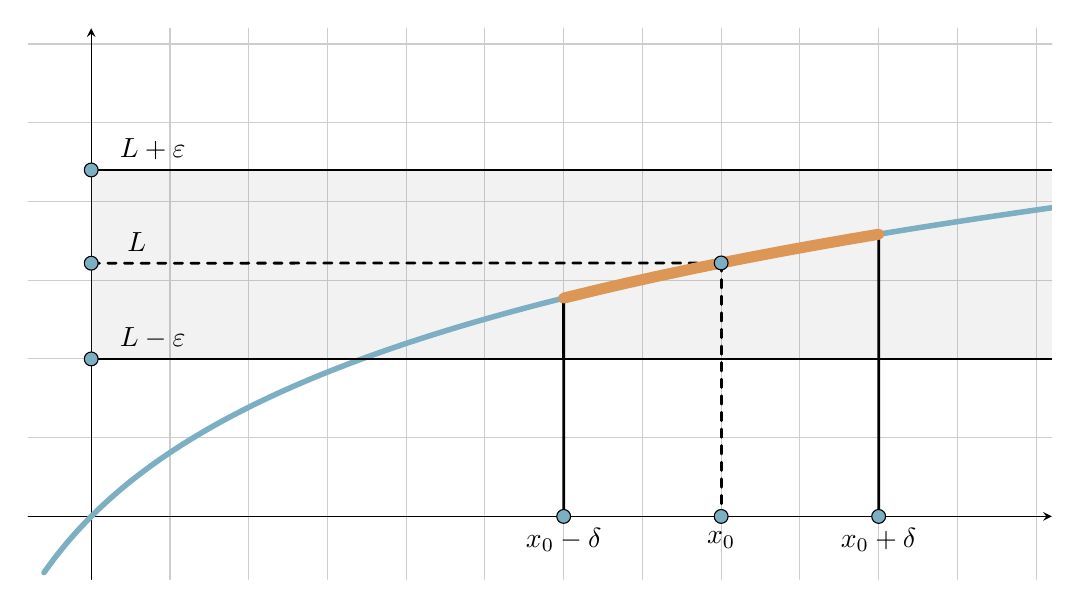
\begin{tikzpicture}[line cap=round,line join=round,>=triangle 45,x=1cm,y=1cm]
   \begin{axis}[
   ticks=none,
   x=2cm, y=2cm,
   axis lines=middle,
   ymajorgrids=true,
   xmajorgrids=true,
   xmin=-0.4, xmax=6.1,
   ymin=-0.4, ymax=3.1]
      \fill[line width=2pt,color=gray,fill=gray,fill opacity=0.1] (0,2.2) -- (8,2.2) -- (8,1) -- (0,1) -- cycle;
      \draw[line width=2pt,color=blue,smooth,samples=100,domain=-0.3:7] plot(\x,{ln((\x)+1)});

      \draw [line width=1pt,dashed] (0,1.6079667094364514) -- (4.000000075430033,1.6094379275201067);
      \draw [line width=1pt,dashed] (4.000000075430033,1.6094379275201067)-- (4,0);
      \draw [line width=1pt] (3,0) -- (2.9996517855796725,1.3862073037254237);
      \draw [line width=1pt] (5,0) -- (5.000842962216623,1.7918999530625097);
      \draw [line width=1pt] (0,2.2) -- (8,2.2);
      \draw [line width=1pt] (8,1) -- (0,1);

      \draw [line width=4pt,color=orange] (2.9996517855796725,1.3862073037254237)-- (3.199034292788041,1.4348545685627394)-- (3.399609048748734,1.4815156844194872)-- (3.5985123484097543,1.5257328486695583)-- (3.799087104370447,1.5684257132365922)-- (4.000000075430033,1.6094379275201067)-- (4.200236616291833,1.6487041276851904)-- (4.402482828552198,1.6868586309676052)-- (4.6013861282132185,1.7230140900075834)-- (4.8002894278742385,1.7579078176649696)-- (5.000842962216623,1.7918999530625097);

      \draw [fill=blue] (0,2.2) circle (2.5pt);
      \draw (0.39, 2.33) node {\(L + \varepsilon\)};
      \draw [fill=blue] (0,1.6079667094364514) circle (2.5pt);
      \draw (0.29, 1.7408231122516713) node {\(L\)};
      \draw [fill=blue] (0,1) circle (2.5pt);
      \draw (0.39, 1.13) node {\(L - \varepsilon\)};

      \draw [fill=blue] (4.000000075430033,1.6094379275201067) circle (2.5pt);

      \draw [fill=blue] (5,0) circle (2.5pt);
      \draw (5, -0.15) node {\(x_0 + \delta\)};
      \draw [fill=blue] (4,0) circle (2.5pt);
      \draw (4, -0.15) node {\(x_0\)};
      \draw [fill=blue] (3,0) circle (2.5pt);
      \draw (3, -0.15) node {\(x_0 - \delta\)};
   \end{axis}
\end{tikzpicture}

   \end{center}

   \begin{example}[Constant Function]
      Let \(f: I \to \mathbb{R}~\text{with}~x \mapsto c\).
      It holds that \(\forall x \in I: f(x) = c\).
      This means that for any \(\varepsilon > 0\) it holds that \(\forall x \in I, x_0 \in I: |f(x) - f(x_0)| = 0 < \varepsilon\).
      Therefor is a constant function continuous on \(I\).
   \end{example}
   \begin{example}
      Let \(f: I \to \mathbb{R}~\text{with}~x \mapsto x^2\).
      We set \(\delta := \sqrt\varepsilon\), then is
      \[\forall \varepsilon > 0: (\forall x \in I: |x - 0| = |x| < \delta \implies |x^2 - 0^2| = |x|^2 < \varepsilon)\]
      \(f\) continuous at \(x_0 = 0\).
   \end{example}
   \begin{example}
      Let
      \[f: \mathbb{R} \to \mathbb{R}~\text{be defined through}~f(x) = \begin{cases}0: & x \leq 0\\ 1: & x > 0\end{cases}\]
      \(f\) is discontinuous at \(x_0 = 0\) since for \(\varepsilon = \frac{1}{2}\) we can't choose \(\delta > 0\) such that
      \[\forall x \in \mathbb{R}: |x - 0| < \delta \implies |f(x) - f(0)| < \varepsilon\]
      because for any choice of \(\delta\), \(\exists x \in \mathbb{R}: 0 < x < \delta \implies f(x) = 1 > \varepsilon\).
   \end{example}
   \begin{example}
      Let
      \[f: \mathbb{Q} \to \mathbb{R}~\text{be defined through}~f(x) = \begin{cases}0: & x^2 < 2\\ 1: & x^2 > 2\end{cases}\]
      However since \(\sqrt{2} \not\in \mathbb{Q}\) is the point where \(f\) jumps not in the domain.
      Now let \(\varepsilon > 0\) and for an arbitrary \(x_0 \in \mathbb{Q}\) we set \(\delta = |x_0 - \sqrt{2}|\).
      \[\forall x \in \mathbb{Q}: |x - x_0| < \delta \implies f(x) = f(x_0) \implies |f(x) - f(x_0)| = 0 < \varepsilon\]
   \end{example}
   % TODO: what?
   \begin{example}
      Let \(f: \mathbb{R} \setminus \{0\} \to \mathbb{R}~\text{with}~x \mapsto \frac{1}{x}\).
      Let \(x_0 \neq 0\) and \(\varepsilon > 0\).
      For some \(|x| < \frac{|x_0|}{2}\) holds
      \[|f(x) - f(x_0)| = \left|\frac{1}{x} - \frac{1}{x_0}\right| = \left|\frac{x_0-x}{x \cdot x_0}\right| = |x-x_0| \frac{1}{|x_0||x|} \leq \frac{2}{|x_0|^2} |x-x_0|\]
      so we choose \(\delta = \min\left(\frac{|x_0|}{2}, \varepsilon \frac{|x_0|^2}{2}\right)\), then is
      \[|x-x_0| < \delta \implies |x| > \frac{|x_0|}{2} \land |x-a| < \varepsilon \frac{|x_0|^2}{2}\]
      because \(|x| = |x-x_0+x_0| > |x_0| - |x-x_0| > |x_0| - \delta \geq \frac{|x_0|}{2}\) so it follows that
      \[|f(x) - f(x-0)| < \frac{2}{|x_0|^2} |x-a| < \frac{2\delta}{|x_0|^2} \leq \frac{2}{|x_0|^2} \cdot \frac{\varepsilon|x_0|^2}{2} = \varepsilon\]
   \end{example}
   \begin{example}
      Let \(f: \mathbb{R} \to \mathbb{R}\)
      \[f(x) = \begin{cases}0 & x \in \mathbb{R}\setminus \mathbb{Q}\\ \frac{1}{q} & x = \frac{p}{q} \land p \nmid q\end{cases}\]
      \(f\) is continuous at \(\forall x_0 \in \mathbb{R}\setminus\mathbb{Q}\) and discontinuous at \(\forall x_0 \in \mathbb{Q}\).

      Let \(x_0 \in \mathbb{R} \setminus \mathbb{Q}\).
      W.l.o.g. we can assume that \(x_0 > 0\).
      We can find \(n \in \mathbb{N}: x_0 < n\).
      Now let \(\varepsilon > 0\).
      We find \(\mathcal{Q} \in \mathbb{N}_+: \frac{1}{\mathcal{Q}} < \varepsilon\).
      Then we set
      \[\delta := \min\left\{\left|x_0 - \frac{p}{q}\right|: (p, q \in \mathbb{N}: 1 \leq q \leq \mathcal{Q} \land 0 \leq p \leq 2nq)\right\}\]
      Since \(x_0 \not\in \mathbb{Q} \implies \delta > 0\).
      Is \(|x-x_0|< \delta\) we distinguish two cases
      \[x \in \mathbb{R} \setminus \mathbb{Q} \implies f(x) = 0 = f(x_0) \implies |f(x) - f(x_0)| < \varepsilon\]
      \[x \in \mathbb{Q} \implies x = \frac{p_1}{q_1}~\text{for}~p_1, q_1 \in \mathbb{N}\]
      (this holds because \(\delta < |x_0| = x_0 \land |x-x_0| < \delta \implies x > 0\)).
      According to our definition of \(\delta\) either \(q_1 > \mathcal{Q}\) or \(q_1 \leq \mathcal{Q} \land p_1 > 2nq_1\).
      In the second case would be \(x = \frac{p_1}{q_1} > 2n > 2x_0 \implies |x-x_0| > x_0\) whichwould be a contradiction to \(|x-x_0| < \delta < x_0\).
      Thus it must hold that \(q_1 > \mathcal{Q} \implies f(x) = \frac{1}{q_1} < \frac{1}{\mathcal{Q}} < \varepsilon\).
      Since \(f(x_0) = 0 \implies |f(x) - f(x_0)| < \varepsilon\) which means for \(x \in \mathbb{R} \setminus \mathbb{Q}\) is \(f\) continuous.
   \end{example}

   \begin{proposition}[Continuity as property of Sequences]\label{pro:image_of_seq_conv}
      Let \(I \subset \mathbb{R}\) and \(f: I \to \mathbb{R}\).

      \(f\) is continuous at \(x \in I\) iff for all sequences \(x_n \in I\) holds
      \[x_n \to x \implies f(x_n) \to f(x)\]
   \end{proposition}

   \begin{proposition}[Function Calculation Rules]\label{pro:sequence_operations_for_functions}
      Let \(I \subset \mathbb{R}\) and \(f, g: I \to \mathbb{R}\) be continuous at \(x_0 \in I\). Then are
      \[f + g: I \to \mathbb{R} \quad\text{where}\quad (f + g)(x) := f(x) + g(x)\]
      \[f \cdot g: I \to \mathbb{R} \quad\text{where}\quad (f \cdot g)(x) := f(x) \cdot g(x)\]
      also continuous at \(x_0 \in I\).
      For \(g(x_0) \neq 0\) is also
      \[\frac{f}{g}: I \to \mathbb{R} \quad\text{where}\quad \left(\frac{f}{g}\right)(x) := \frac{f(x)}{g(x)}\]
      continuous at \(x_0 \in I\).
   \end{proposition}
   \begin{proof}
      Follows from \cref{pro:R_field_operations} which we can use according to \cref{pro:image_of_seq_conv}.
   \end{proof}

   \begin{corollary}[Polynomials are Continuous]
      Polynomials are everywhere continuous, this means that \textit{rational functions}
      \[f(x) := \frac{p(x)}{q(x)}\]
      of two polynomials \(p, q\) are continuous on \(\{x \mid g(x) \neq 0\}\).
   \end{corollary}
   \begin{proof}
      Follows from \cref{pro:sequence_operations_for_functions}.
   \end{proof}

   \begin{proposition}[Continuous Compositions]\label{pro:contin_continuation}
      Let \(I_1, I_2 \subset \mathbb{R}\), \(f: I_1 \to \mathbb{R}\) and \(g: I_2 \to \mathbb{R}\).

      If \(\im(f) \subset I_2\), \(f\) continuous at \(x_0 \in I_1\) and \(g\) at \(f(x_0) \in I_2\) then is
      \[g \circ f: I_1 \to \mathbb{R}~\text{continuous at}~x_0\]
   \end{proposition}
   \begin{example}
      Let \(f(x) = x^2 + 3\) and \(g(x) = \sqrt{x}\).

      \(h(x) = (g \circ f)(x) = \sqrt{x^2 + 3}\) is continuous since \(f\) and \(g\) both are.
   \end{example}

   \subsection{Limits of Functions}
   \begin{definition}[Limit Point]
      Let \(I \subset \mathbb{R}\).
      An \(a \in \mathbb{R}\) is a limit point of \(I\) if for all \textit{punctured intervals}
      \[U := (a-\varepsilon; a) \cup (a; a+\varepsilon) \quad\text{holds}\quad \forall \varepsilon > 0: U \cap I \neq \emptyset\]
   \end{definition}
   \begin{remark}
      In other words, a limit point --- also called a \textit{cluster} or \textit{accumulation point} (not to confuse with \textit{adherent point}) --- is a point that can be ''approximated`` by points in \(I\) in the sense that every \textit{neighbourhood} \(U\) of \(x\) also contains a point of \(I\) other than \(x\) itself.
      This concept is closely related to cluster points of sequences.
      A limit point of a set \(I\) does not itself have to be an element of \(I\).
   \end{remark}
   \begin{remark}
      Let \(a\) be a limit point of \(I\).
      Every \(U\) contains infinitely many elements of \(I\).

      If \(U \cap I = \{x_1, \ldots, x_n\}\) was finite then would through \(\delta := \min\{|a - x_1|, \ldots, |a - x_n|\} > 0\) follow that
      \[\big((a-\delta;a) \cup (a;a+\delta)\big) \cap I = \emptyset\]
      which would be a contradiction to the fact that \(a\) is a limit point of \(I\).
   \end{remark}
   \begin{example}
      Every \(x \in \mathbb{R}\) is a limit point of \(\mathbb{R}\), \(\mathbb{Q}\) and \(\mathbb{R}\setminus\mathbb{Q}\).
      But no \(x \in \mathbb{R}\) is a limit point of \(\mathbb{Z}\).
   \end{example}

   \begin{proposition}\label{pro:limit_point_convergent_seq}
      Let \(I \subset \mathbb{R}\).

      \(x \in \mathbb{R}\) is a limit point of \(I\) iff \(\exists (x_n)_{n \in \mathbb{N}} \subset (I \setminus \{x\}): x_n \to x\).
   \end{proposition}

   \begin{definition}[Limit of a Function]
      Given a limit point \(a \in \mathbb{R}\) of \(I \subset \mathbb{R}\) and \(f: I \to \mathbb{R}\).
      \[\lim_{x \to a} f(x) = b \qquad\text{is the limit of}~f(x)~\text{as}~x \to a~\text{if}\]
      \[\forall \varepsilon > 0~\exists \delta > 0: (x \in I: 0 < |x-a| < \delta \implies |f(x) - b| < \varepsilon)\]
   \end{definition}
   \begin{remark}
      If \(\lim_{x \to a} f(x)\) exists it is unique and the usual calculation rules hold.
      Also
      \[\forall x \in (a - \delta; a) \cup (a; a + \delta): f(x) \leq g(x) \implies \lim_{x \to a} f(x) \leq \lim_{x \to a} g(x)\]
   \end{remark}

   \begin{proposition}[Function Limit = Sequence Limit]
      Let \(a \in I\) a limit point of \(I \subset \mathbb{R}\) and let \(f: I \to \mathbb{R}\).
      \[\lim_{x \to a} f(x) = b \iff f(x_n) \to b,~\forall (x_n) \in I \setminus \{a\}: x_n \to a\]
   \end{proposition}
   \begin{proof}
      Similar as proof of \cref{pro:image_of_seq_conv}.
   \end{proof}
   \begin{remark}[Calculation Rules for Function Limits]
      This proposition allows us to calculate the limit of functions through the limit of sequences.
      \[\lim_{x \to a} (f(x) + g(x)) = \lim_{x \to a} f(x) + \lim_{x \to a} g(x)\]
      \[\lim_{x \to a} (f(x) \cdot g(x)) = \lim_{x \to a} f(x) \cdot \lim_{x \to a} g(x)\]
      \[\lim_{x \to a} \frac{f(x)}{g(x)} = \frac{\lim_{x \to a} f(x)}{\lim_{x \to a} g(x)}\]
   \end{remark}
   \begin{example}[\(f(x) = x^3\)]
      It holds that \(\lim_{x \to 0} f(x) = 0\) because 0 is a limit point in \(\mathbb{R}\).
      For any \(\varepsilon > 0\) we can set \(\delta := \sqrt[3]{\varepsilon}\) and have
      \[\forall x \in I: 0 < |x - 0| < \delta \implies |x^3 - 0| < \varepsilon\]
   \end{example}
   \begin{example}[\(f(x) = \sin \frac{1}{x}\)]
      If we regard the sequence \((x_n)_{n \in \mathbb{N}} = \frac{1}{\pi n}\) then holds that \(x_n \to 0\).
      But \(\sin \frac{1}{x_n} = \sin(\pi n) = (-1)^n\) does not converge, hence \(\lim_{x \to 0} \sin \frac{1}{x}\) does not exist.
   \end{example}
   \begin{example}[\(f(x) = \sin x \frac{1}{x}\)]
      Since \(\sin \frac{1}{x} \leq 1 \implies |x \sin \frac{1}{x}| \leq |x|\) and so \(|x \sin \frac{1}{x} < \varepsilon\) if \(|x| < \varepsilon =: \delta\) we see that \(\lim_{x \to 0} x \sin \frac{1}{x} = 0\).
   \end{example}
   \begin{example}
      Let \(f: \mathbb{R} \to \mathbb{R}\) be defined through
      \[f(x) = \begin{cases}1 & x \in \mathbb{Q}\\ 0& x \in \mathbb{R} \setminus \mathbb{Q}\end{cases}\]
      \(\lim_{x \to a} f(x)\) doesn't exists for any \(a \in \mathbb{R}\).
   \end{example}

   \begin{proposition}[Limit Point = Function Limit]
      Let \(a \in I\) a limit point of \(I \subset \mathbb{R}\) and \(f: I \to \mathbb{R}\).

      \(f\) must have a limit and \(f\) is continuous at \(a\) iff \(\lim_{x \to a} f(x) = f(a)\).
   \end{proposition}
   \begin{proof}
      Follows from the \cref{def:continuity}.
   \end{proof}

   \begin{proposition}[Continuous Continuation]\label{pro:continuous_contin}
      Let \(a\) be a limit point of \(I \subset \mathbb{R}\) and \(f\) at least be defined on \(I \setminus \{a\}\).
      Assume there exists \(b := \lim_{x \to a} f(x)\).

      We define a new function \(\widetilde{f}\) on \(I\) through
      \[\widetilde{f}(x) = \begin{cases} f(x)& x \in I \setminus \{a\}\\b & x = a\end{cases}\]
      then is \(\widetilde{f}\) is continuous at \(a\).
   \end{proposition}
   \begin{example}
      Let \(f: \mathbb{R} \setminus \{1\} \to \mathbb{R}\) be defined as
      \[f(x) = \frac{x^2 - 1}{x - 1}\]
      \[\frac{x^2 - 1}{x - 1} = \frac{(x-1)(x+1)}{x-1} = x+1 \implies \lim_{x \to 1} f(x) = \lim_{x \to 1} x + 1 = 2\]
      The map
      \[\widetilde{f}(x) = \begin{cases}x+1& x \neq 1\\ 2 & x = 1\end{cases}\]
      is continuous at \(x = 1\).
      Because \(f\) as rational function is continuous on \(\mathbb{R} \setminus \{1\}\) is \(\widetilde{f}\) continuous of \(\mathbb{R}\).
   \end{example}

   \begin{definition}[One-Sided Limit]
      Let \(a \in \mathbb{R}\) a limit point of \(I \subset \mathbb{R}\) and \(f: I \to \mathbb{R}\).
      \[\text{Left-handed Limit:}\quad \lim_{x \uparrow a}f(x) = \lim_{x \to a} f|_{I_a^-}\quad\text{where}\quad I_a^- = I \cap (-\infty; a)\]
      \[\text{Right-handed Limit:}\quad \lim_{x \downarrow a}f(x) = \lim_{x \to a} f|_{I_a^+} \quad\text{where}\quad I_a^+ = I \cap (a; \infty)\]
   \end{definition}
   \begin{remark}
      One-sided limits exist always.
   \end{remark}
   \begin{remark}
      \[\lim_{x \uparrow a} f(x) = b \iff \forall \varepsilon~\exists \delta > 0: (x \in I: a- \delta < x < a \implies |f(x) - b| < \varepsilon)\]
      \[\lim_{x \downarrow a} f(x) = b \iff \forall \varepsilon~\exists \delta > 0: (x \in I: a < x < a + \delta \implies |f(x) - b| < \varepsilon)\]
   \end{remark}
   \begin{example}
      We know that that \(\lim_{x \to 0} f(x)\) does not exist for the following function
      \[f(x) = \begin{cases}0 & x \leq 0\\ 1 & x > 0\end{cases}\]
      but both one-sided limits exist
      \[\lim_{x \uparrow 0} f(x) = 0 \qquad \lim_{x \downarrow 0} f(x) = 1\]
   \end{example}

   \begin{proposition}[\(x \to a = x \uparrow a = x \downarrow a\)]
      Let \(a \in \mathbb{R}\) be a limit point of \(I \subset \mathbb{R}\) and \(f: I \to \mathbb{R}\).
      \[\lim_{x \to a} f(x)~\text{exists} \iff \lim_{x \uparrow a} f(x),~\lim_{x \downarrow a} f(x)~\text{exist and}~\lim_{x \uparrow a} f(x) = \lim_{x \downarrow a} f(x)\]
      In that case holds
      \[\lim_{x \to a} f(x) = \lim_{x \uparrow a} f(x) = \lim_{x \downarrow a} f(x)\]
   \end{proposition}
   % TODO: copy from exercises
   \begin{proof}
   \end{proof}
   \begin{remark}
      This proposition implies that \(f\) is continuous at \(x_0 \in I\) iff \(\lim_{x \uparrow x_0} f(x)\), \(\lim_{x \downarrow x_0} f(x)\) exist and
      \[f(x_0) = \lim_{x \uparrow x_0} f(x) = \lim_{x \downarrow x_0} f(x)\]
   \end{remark}

   \begin{proposition}\label{pro:one_sided_lim_incr}
      Let \(f: [a; b] \to \mathbb{R}\) be increasing and \(c \in (a; b)\), then is
      \[f(c^-) := \lim_{x \uparrow c} f(x) = \sup\{f(x) \mid x < c\} \quad\text{and}\quad f(c^+) := \lim_{x \downarrow c} f(x) = \inf\{f(x) \mid x > c\}\]
      \[f(c^-) \leq f(c) \leq f(c^+)\]
   \end{proposition}
   \begin{remark}
      It it follows that \(f\) is continuous at \(c\) iff \(f(c^-) = f(c^+)\).
   \end{remark}

   \begin{center}
      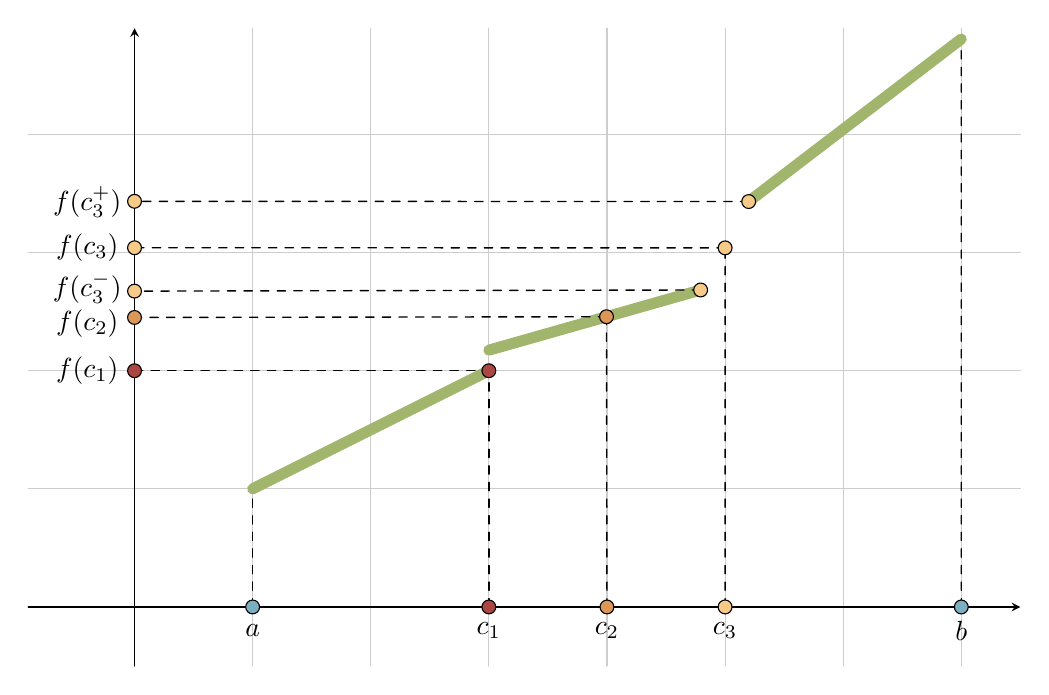
\begin{tikzpicture}[line cap=round,line join=round,>=triangle 45,x=1cm,y=1cm]
   \begin{axis}[
   ticks=none,
   x=1.5cm,y=1.5cm,
   axis lines=middle,
   ymajorgrids=true,
   xmajorgrids=true,
   xmin=-0.9, xmax=7.5,
   ymin=-0.5, ymax=4.9]

      \draw [line width=0.5pt,dashed] (7,0)-- (6.999347663225158,4.808375546139909);
      \draw [line width=0.5pt,dashed] (1,0)-- (1,1);

      \draw [fill=blue] (1,0) circle (2.5pt);
      \draw (1, -0.2) node {\(a\)};
      \draw [fill=blue] (7,0) circle (2.5pt);
      \draw (7, -0.2) node {\(b\)};

      \draw [line width=4pt, color=green] (1,1)-- (3,2);
      \draw [line width=4pt, color=green] (3,2.1741614881443576)-- (4.792997852271268,2.683669545697946);
      \draw [line width=4pt, color=green] (5.2,3.4324016315214996)-- (6.999347663225158,4.808375546139909);

      \draw [line width=0.5pt, dashed] (0,2) -- (3,2);
      \draw [line width=0.5pt, dashed] (4,0)-- (3.9960481823364784,2.4572039769957392);
      \draw [line width=0.5pt, dashed] (3.9960481823364784,2.4572039769957392)-- (0,2.451192594490506);
      \draw [line width=0.5pt, dashed] (3,0)-- (3,2);
      \draw [line width=0.5pt, dashed] (5,0)-- (5.000511853340461,3.0404031012859707);
      \draw [line width=0.5pt, dashed] (5.000511853340461,3.0404031012859707)-- (0,3.041252304933857);
      \draw [line width=0.5pt, dashed] (4.792997852271268,2.683669545697946)-- (0,2.674060594245076);
      \draw [line width=0.5pt, dashed] (5.2,3.4324016315214996)-- (0,3.4344860163850863);

      \draw [fill=red] (3,0) circle (2.5pt);
      \draw (3, -0.2) node {$c_1$};
      \draw [fill=red] (0,2) circle (2.5pt);
      \draw (-0.4, 2) node {$f(c_1)$};
      \draw [fill=red] (3,2) circle (2.5pt);

      \draw [fill=orange] (4,0) circle (2.5pt);
      \draw (4, -0.2) node {$c_2$};
      \draw [fill=orange] (3.9960481823364784,2.4572039769957392) circle (2.5pt);
      \draw [fill=orange] (0,2.451192594490506) circle (2.5pt);
      \draw (-0.4, 2.4) node {$f(c_2)$};

      \draw [fill=yellow] (5,0) circle (2.5pt);
      \draw (5, -0.2) node {$c_3$};
      \draw [fill=yellow] (4.792997852271268,2.683669545697946) circle (2.5pt);
      \draw [fill=yellow] (5.000511853340461,3.0404031012859707) circle (2.5pt);
      \draw [fill=yellow] (5.2,3.4324016315214996) circle (2.5pt);

      \draw [fill=yellow] (0,2.674060594245076) circle (2.5pt);
      \draw (-0.4, 2.7) node {\(f(c_3^-)\)};
      \draw [fill=yellow] (0,3.041252304933857) circle (2.5pt);
      \draw (-0.4, 3.04) node {\(f(c_3)\)};
      \draw [fill=yellow] (0,3.4344860163850863) circle (2.5pt);
      \draw (-0.4, 3.43) node {\(f(c_3^+)\)};
   \end{axis}
\end{tikzpicture}

   \end{center}
   \begin{example}
      \[f(c_1) = \lim_{x \uparrow c_1} f(x) = f(c_1^-) < f(c_1^+)\]
      \[f(c_2) = \lim_{x \to c_2} f(x) = f(c_2^-) = f(c_2^+)\]
      \[f(c_3^-) < f(c_3) < f(c_3^+)\]
   \end{example}

   \begin{definition}[Improper Limit of Functions]
      Let \(a \in \mathbb{R}\) be a limit point of \(I \subset \mathbb{R}\).
      \[\lim_{x \to a} f(x) = \infty \quad\text{if}\quad \forall \varepsilon > 0~\exists \delta > 0: (\forall x \in I: 0 < |x - a| < \delta \implies f(x) > \varepsilon)\]
      \[\lim_{x \to a} f(x) = -\infty \quad\text{if}\quad \forall \varepsilon > 0~\exists \delta > 0: (\forall x \in I: 0 < |x - a| < \delta \implies -f(x) > \varepsilon)\]
   \end{definition}
   \begin{remark}
      We say \(\infty\) is a limit point of \(I \subset \mathbb{R}\) if \(\forall R > 0: (R; \infty) \cap I \neq \emptyset\).

      Now let \(f: I \to \mathbb{R}\) and \(\infty\) a limit point of \(I\) (\(I\) is unbounded above).
      \[\lim_{x \to \infty} f(x) = b \quad\text{if\quad} \forall \varepsilon > 0 \exists r > 0: (x \in I: x > r \implies |f(x) - b| < \varepsilon)\]
      \(\lim_{x \to -\infty} f(x) = b\) is defined analogously
   \end{remark}
   \begin{example}[\(f(x) = \frac{1}{x}\)]
      \[\lim_{x \downarrow 0} f(x) = \infty \quad\text{and}\quad \lim_{x \uparrow 0} f(x) = -\infty \quad\text{but}\quad \lim_{x \to 0} f(x)~\text{doesn't exist}\]
      however
      \[\lim_{x \to \infty} f(x) = 0~\text{since}~\forall \varepsilon > 0: |\frac{1}{x} - 0| = \frac{1}{|x|} < \varepsilon\]
   \end{example}
   \begin{example}
      Let
      \[f(x) = \begin{cases}\frac{1}{x^2} & x \neq 0\\ 25 & x=0\end{cases}\]
      we see \(\lim_{x \to 0} f(x) = \infty\).
      The point \(x = 0\) is irrelevant since \(x\) is only close to 0 but never exactly 0.
   \end{example}

   % TODO: where to put
   \begin{remark}[Fundamental Limits]
      \[\lim_{x \to \infty} (1 + \frac{1}{x})^x = e \quad\text{and}\quad \lim_{x \to 0} (1 + x)^{\frac{1}{x}} = e\]
      From this follows (not trivially) a neat trick:
      \[\lim_{x \to a} (1 + \frac{1}{\ast})^* = e \quad\text{and}\quad \lim_{x \to a} (1 + \ast)^{\frac{1}{\ast}} = e\]
      where \(\ast\) is an arbitrary term in \(x\) with \(\lim_{x \to a} \ast = \infty\) respectively \(\lim_{x \to a} \ast = 0\).
   \end{remark}

   \subsection{Continuous Functions on Intervals}
   \begin{theorem}[Intermediate Value Theorem]\label{thm:intmd_value}
      Let \(f: [a; b] \to \mathbb{R}\) be continuous with \(f(a) < 0 < f(b)\).
      \[\exists c \in (a;b): f(c) = 0\]
   \end{theorem}
   \begin{remark}
      The same statement holds for \(f(b) < 0 < f(a)\).
   \end{remark}

   \begin{proposition}[Continuous Inverse]\label{pro:inv_cont}
      Let \(f: [a; b] \to \mathbb{R}\) be strictly increasing and continuous.

      Furthermore let \(c = f(a)\), \(d = f(b)\), then is
      \[f: [a;b] \to [c;d]~\text{bijective and} \quad f^{-1}: [c;d] \to [a;b]~\text{continuous}\]
   \end{proposition}
   \begin{remark}
      In words: the inverse of a continuous, strictly monotonic function is continuous.
   \end{remark}

   \begin{theorem}[Extreme Value Theorem]\label{thm:extreme_value}
      Let \(f: [a; b] \to \mathbb{R}\) be continuous.
      \[\exists m, M \in [a; b]: \big(\forall x \in [a; b]: f(m) \leq f(x) \leq f(M)\big)\]
   \end{theorem}
   \begin{remark}
      This theorem states that if \(f\) is continuous, it follows that \(f\) is bounded and takes the values of \(\inf f(x)\) and \(\sup f(x)\), hence it must attain a maximum and a minimum, each at least once.
   \end{remark}

   \begin{definition}[Lipschitz Continuity]
      Given \(I \subset \mathbb{R}\) and \(f: I \to \mathbb{R}\).
      \[\exists L > 0~\forall x, y \in I: |f(x) - f(y)| \leq L \cdot |x - y|\]
   \end{definition}
   \begin{remark}
      Intuitively, a Lipschitz continuous function is limited in how fast it can change.
      For every pair of points on the graph of \(f\), the absolute value of the slope of the line connecting them is not greater than \(L\).
      \[\left|\frac{f(x) - f(y)}{x - y}\right| \leq L\]
   \end{remark}

   \begin{definition}[Uniform Continuity]
      Given \(I \subset \mathbb{R}\) and \(f: I \to \mathbb{R}\).
      \[\forall \varepsilon > 0~\exists \delta > 0: (\forall x,y \in I: |x - y| < \delta \implies |f(x) - f(y)| < \varepsilon)\]
   \end{definition}
   \begin{remark}
      The difference to regular continuity is that for uniform continuity \(\delta\) does not depend on \(x_0\) but only on \(\varepsilon\).
      This means that the same \(\delta\) must be applicabale to all \(x \in I\).
   \end{remark}
   \begin{remark}
      A function \(f\) is uniformly continuous if, it is possible to guarantee that \(f(x)\) and \(f(y)\) be as close to each other as we please by requiring only that \(x\) and \(y\) are sufficiently close to each other.
   \end{remark}
   \begin{example}
      \(f(x) = x^2\) is uniformly continuous on \([0; 1]\) because
      \[|x^2 - y^2| = |(x-y)(x+y)| \leq |x + y| \cdot |x - y| \leq 2|x - y| \leq \varepsilon\]
      with \(|x - y| \leq \frac{\varepsilon}{2} =: \delta\).

      % TODO: what?
      However \(f\) is not uniformly continuous on \([0; \infty)\) because for some fixed \(|x - y|\) can \(|x^2 - y^2| = |x - y||x + y|\) get arbitrary large if we choose \(x, y\) large enough.
   \end{example}

   \begin{theorem}[Uniform = Regular Continuity]\label{thm:uniform=regular_cont}
      Let \(f: [a;b] \to \mathbb{R}\) be continuous,

      then is \(f\) also uniformly continuous on \([a;b]\).
   \end{theorem}
   \begin{remark}
      This theorem is only applicable to functions which are defined on closed and bounded intervals, so not to \(f: (0;1] \to \mathbb{R}\) for example.

      From this theorem also follows that \(f: [0; 1] \to \mathbb{R}\) defined through \(x \mapsto \sqrt{x}\) is uniformly continuous.
      This means that uniform continuity is weaker than Lipschitz continuity.
   \end{remark}

   \begin{remark}
      \[f~\text{Lipschitz continuous} \implies f~\text{uniformly continuous} \implies f~\text{continuous}\]
   \end{remark}

   % TODO: fixpoint and continuity exercises?

   \subsection{Function Sequence and Continuity}
   \begin{definition}[Function Sequence]
      Given \(I \subset \mathbb{R}\) and \(f_n: I \to \mathbb{R}\).
      \[(f_n)_{n \in \mathbb{N}} = f_1, f_2, \ldots f_n\]
   \end{definition}

   \begin{definition}[Pointwise Convergence of Function Sequence]
      A function sequence \((f_n)_{n \in \mathbb{N}}\) converges pointwise to \(f: I \to \mathbb{R}\) if
      \[\forall x \in I: f_n(x) \to f(x)\]
   \end{definition}
   \begin{example}
      Let \(I = [0;1]\) and \((f_n)_{n \in \mathbb{N}}: I \to \mathbb{R}\) be defined through \(f_n(x) = x^n\).

      For \(x \in [0;1)\) holds \(x^n \xrightarrow{n \to \infty} 0\) and at \(x = 1\) is \(x^n \to 1\).
      We define
      \[f(x) = \begin{cases}0:& x \in [0; 1)\\ 1: & x = 1\end{cases}\]
      and see that \(\forall x \in I: f_n(x) \to f(x)\).
      From this example we also see that continuity is not preserved with pointwise convergence as \(\forall n \in \mathbb{N}: f_n\) is continuous but \(f\) is not.
   \end{example}

   \begin{center}
      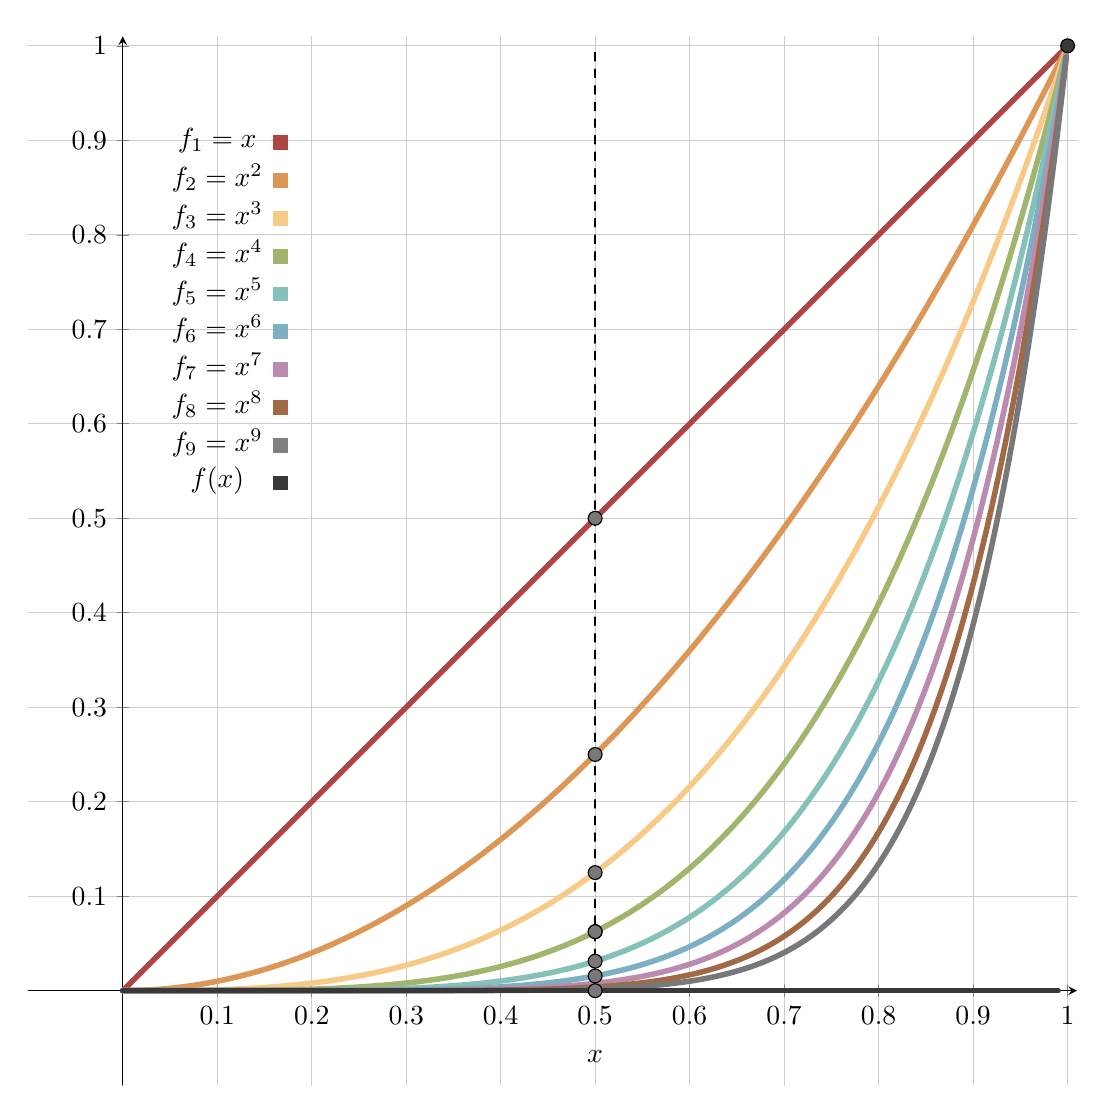
\begin{tikzpicture}[line cap=round,line join=round,>=triangle 45,x=1cm,y=1cm]
\begin{axis}[
   x=12cm,y=12cm,
   axis lines=middle,
   ymajorgrids=true,
   xmajorgrids=true,
   xmin=-0.1, xmax=1.01,
   ymin=-0.1, ymax=1.01,
   xtick={0,0.1,...,1},
   ytick={0,0.1,...,1},]

   \draw[line width=2pt,color=red,smooth,samples=100,domain=0:1] plot(\x,{(\x)});
   \draw[line width=2pt,color=orange,smooth,samples=100,domain=0:1] plot(\x,{(\x)^(2)});
   \draw[line width=2pt,color=yellow,smooth,samples=100,domain=0:1] plot(\x,{(\x)^(3)});
   \draw[line width=2pt,color=green,smooth,samples=100,domain=0:1] plot(\x,{(\x)^(4)});
   \draw[line width=2pt,color=cyan,smooth,samples=100,domain=0:1] plot(\x,{(\x)^(5)});
   \draw[line width=2pt,color=blue,smooth,samples=100,domain=0:1] plot(\x,{(\x)^(6)});
   \draw[line width=2pt,color=purple,smooth,samples=100,domain=0:1] plot(\x,{(\x)^(7)});
   \draw[line width=2pt,color=brown,smooth,samples=100,domain=0:1] plot(\x,{(\x)^(8)});
   \draw[line width=2pt,color=grey,smooth,samples=100,domain=0:1] plot(\x,{(\x)^(9)});
   \draw [line width=2pt, color=black] (0,0) -- (0.99,0);
   \draw [fill=black] (1,1) circle (2.5pt);

   \draw (0.1, 0.9) node {\(f_1 = x\)};
   \filldraw[color=red] (0.16, 0.89) rectangle ++(5pt,5pt);
   \draw (0.1, 0.86) node {\(f_2 = x^2\)};
   \filldraw[color=orange] (0.16, 0.85) rectangle ++(5pt,5pt);
   \draw (0.1, 0.82) node {\(f_3 = x^3\)};
   \filldraw[color=yellow] (0.16, 0.81) rectangle ++(5pt,5pt);
   \draw (0.1, 0.78) node {\(f_4 = x^4\)};
   \filldraw[color=green] (0.16, 0.77) rectangle ++(5pt,5pt);
   \draw (0.1, 0.74) node {\(f_5 = x^5\)};
   \filldraw[color=cyan] (0.16, 0.73) rectangle ++(5pt,5pt);
   \draw (0.1, 0.70) node {\(f_6 = x^6\)};
   \filldraw[color=blue] (0.16, 0.69) rectangle ++(5pt,5pt);
   \draw (0.1, 0.66) node {\(f_7 = x^7\)};
   \filldraw[color=purple] (0.16, 0.65) rectangle ++(5pt,5pt);
   \draw (0.1, 0.62) node {\(f_8 = x^8\)};
   \filldraw[color=brown] (0.16, 0.61) rectangle ++(5pt,5pt);
   \draw (0.1, 0.58) node {\(f_9 = x^9\)};
   \filldraw[color=gray] (0.16, 0.57) rectangle ++(5pt,5pt);
   \draw (0.1, 0.54) node {\(f(x)\)};
   \filldraw[color=black] (0.16, 0.53) rectangle ++(5pt,5pt);

   \draw [line width=0.5pt,dashed] (0.5,0) -- (0.5,1);
   \draw [fill=grey] (0.5,0.5) circle (2.5pt);
   \draw [fill=grey] (0.5,0.25) circle (2.5pt);
   \draw [fill=grey] (0.5,0.125) circle (2.5pt);
   \draw [fill=grey] (0.5,0.0625) circle (2.5pt);
   \draw [fill=grey] (0.5,0.0625) circle (2.5pt);
   \draw [fill=grey] (0.5,0.03125) circle (2.5pt);
   \draw [fill=grey] (0.5,0.015625) circle (2.5pt);
   \draw [fill=grey] (0.5,0) circle (2.5pt);
   \draw (0.5, -0.07) node {\(x\)};
   \end{axis}
\end{tikzpicture}

   \end{center}

   \begin{definition}[Uniform Convergence of Function Sequence]
      A function sequence \((f_n)\) with \(f_n: I \to \mathbb{R}\) converges uniformly to \(f: I \to \mathbb{R}\) if
      \[\forall \varepsilon > 0~\exists n_0 \in \mathbb{N}: \forall n > n_0: (x \in I \implies |f_n(x) - f(x)| < \varepsilon)\]
   \end{definition}
   \begin{remark}
      Equivalently is \(f_n \to f\) uniformly convergent if
      \[\sup_{x \in I} |f_n(x) - f(x)| \xrightarrow{n \to \infty} 0 \quad\text{or}\quad f(x) = \lim_{n \to \infty} f_n(x)\]
      \[\limsup_{x \in I} |f_n(x) - f(x)| = 0\]
      \(f_n \to f\) uniformly implies \(f_n \to f\) pointwise.
   \end{remark}
   % TODO: copy ecercise week 8
   \begin{example}
      \(f_n(x) = x^n\) converges uniformly to \(0\) on \([0;\frac{1}{2}]\).
      \[\sup_{x \in [0; \frac{1}{2}]} x^n = \left(\frac{1}{2}\right)^n = \frac{1}{2^n} \to 0\]

      But \(f_n\) doesn't converge uniformly on \([0; 1]\).
      Suppose \(\exists f: [0;1] \to [0;1]\) where \(f_n \to f\) uniformly.
      Then \(f_n \to f\) also pointwise which means \(x \in [0;1): f(x) = 0\) and \(x = 1: f(1) = 1\).
      But since
      \[\sup_{x \in [0;1]} |f_n(x) - f(x)| \geq \left(1 - \frac{1}{n^2}\right)^n \to 0\]
      is the convergence not uniform.
   \end{example}

   \begin{proposition}\label{pro:cont_func}
      Let \(I \subset \mathbb{R}\) and \(\forall n \in \mathbb{N}: f_n: I \to \mathbb{R}\) be continuous and \(f: I \to \mathbb{R}\) such that \(f_n \to f\) uniformly, then is \(f\) continuous.
   \end{proposition}
   \begin{remark}
      This proposition states that continuity is preserved with uniform convergence.
   \end{remark}

   \begin{proposition}[Cauchy criterion for Function Sequencces]\label{pro:cauchy_func_seq}
      Let \(I \subset \mathbb{R}\) and a function sequence \(f_n: I \to \mathbb{R}\), then is \(f_n\) uniform convergent iff
      \begin{equation}\label{eq:cauchy_func_seq}
         \forall \varepsilon > 0~\exists n_0 \in \mathbb{N}: \forall m,n > n_0: (\forall x \in I \implies |f_n(x) - f_m(x)| < \varepsilon)
      \end{equation}
   \end{proposition}
   \begin{remark}
      The condition \cref{eq:cauchy_func_seq} is equivalent to
      \[\forall \varepsilon > 0 \exists n_0 \in \mathbb{N}: m,n > n_0 \implies \sup_{x \in I}|f_n(x) - f_m(x)| < \varepsilon\]

      Further holds the cauchy criterion also for function sequences \(f_n: I \to \mathbb{R}^l\) where \(I \subset R^m\).
      We only have to use the absolute value for vectors (norm).
   \end{remark}

   \begin{remark}[Recipe to show Convergence]
      We're looking for the pointwise limit of \(f_n\).
      \begin{enumerate}
         \item If \(f(x)\) is discontinuous then it cannot be uniformly convergent
         \item Calculate \(f(x) = \lim_{n \to \infty} f_n(x),~\forall x \in I\)
         \item Calculate \(\sup_{x \in I} |f_n(x) - f(x)|\)
         \item Calculate \(\lim_{n \to \infty} (\sup_{x \in I} |f_n(x) - f(x)|\)\\
            if this is 0, then is \((f_n)\) uniformly convergent on \(I\)
      \end{enumerate}
   \end{remark}

   \begin{definition}[Pointwise Convergence of Function Series]
      Given \(I \subset \mathbb{R}\) and \(f_n: I \to \mathbb{R}\) for \(n \in \mathbb{N}\).
      \[s_n(x) = \sum_{i=0}^n f_i(x)~\text{converges pointwise} \implies \sum_{i = 0}^\infty f_i(x)~\text{converges pointwise}\]
   \end{definition}

   \begin{definition}[Uniform Convergence of Function Series]
      Given \(I \subset \mathbb{R}\) and \(f_n: I \to \mathbb{R}\) for \(n \in \mathbb{N}\).
      \[s_n(x) = \sum_{i=0}^n f_i(x)~\text{converges uniformly} \implies \sum_{i = 0}^\infty f_i(x)~\text{converges uniformly}\]
   \end{definition}

   \begin{theorem}[Comparison Test for Function Series]\label{thm:maj_func_ser}
      Let \((f_n)_{n \in \mathbb{N}}\) be a function sequence over \(I \subset \mathbb{R}\).
      \[\exists \sum_{n=0}^\infty m_n~\text{convergent}: (\forall n \in \mathbb{N}, x \in I: |f_n(x)| \leq m_n)~\text{then}\]
      \[\sum_{n = 0}^\infty f_n~\text{converges uniformly} \quad\text{and}\quad \forall x \in I: \sum_{n = 0}^\infty f_n(x)~\text{converges absolutely}\]
   \end{theorem}

   \section{Power Series \& Elementary Functions}
   We use power series to define eulers number.

   \subsection{Power Series}
   \begin{definition}[Power Series]\label{def:power_series}
      Given a complex sequence \(a_n\), variable \(z\) and constant \(c\), a power series is a series of functions
      \[f(z) = \sum_{n=0}^\infty a_n (z - c)^n = a_0 + a_1(z - c)^1 + a_2(z - c)^2 + \ldots\]
   \end{definition}
   \begin{remark}
      \(c\) is the center of the \textit{disk of convergence} which is defined as
      In many situations \(c\) is equal to zero and we can write the series as
      \[\sum_{n=0}^\infty a_n z^n = a_0 + a_1z + a_2z^2 + \ldots\]
   \end{remark}

   \begin{definition}[Disk of Convergence]
      Given a power series, its area of convergence is
      \[\left\{z \in \mathbb{C}~\middle|~\sum a_n z^n~\text{converges}\right\}\]
   \end{definition}
   \begin{remark}
      Differently put, it is the set of all points whose distance to \(c\) is strictly less than the radius of the disk of convergence, the \textit{radius of convergence}.
   \end{remark}

   \begin{center}
      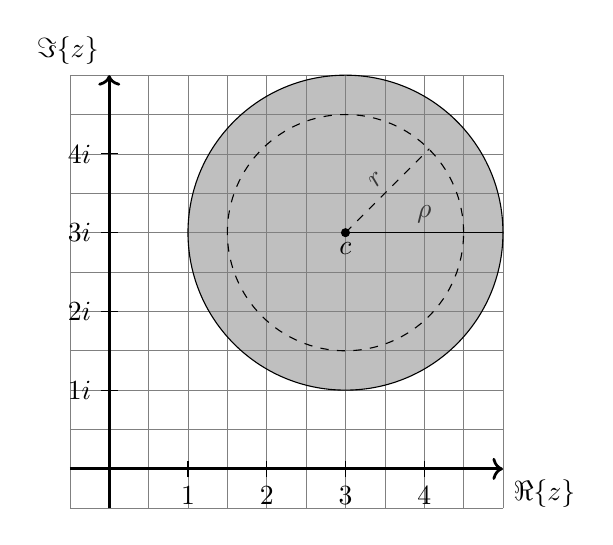
\begin{tikzpicture}
   % coords
   \coordinate (OR) at (0, 0);
   \coordinate (LX) at (-0.5, 0);
   \coordinate (RX) at (5, 0);
   \coordinate (TY) at (0, 5);
   \coordinate (BY) at (0, -0.5);

   % debugging grid
   \coordinate (BL) at (-0.5, -0.5);
   \coordinate (TR) at (5, 5);
   \draw[step=0.5cm, gray, very thin] (BL) grid (TR);

   % coordinate system
   \draw[->][line width=1.00pt] (LX) -- (RX) node[anchor=north west] {\(\Re\{z\}\)};
   \draw[->][line width=1.00pt] (BY) -- (TY) node[anchor=south east] {\(\Im\{z\}\)};
   \foreach \n in {1,2,...,4}{%
      \draw (\n,-3pt) node [below] {$\n$} -- (\n,3pt);
      \draw (-3pt,\n) node [left] {$\n i$} -- (3pt,\n);
   }

   \coordinate (c) at (3,3);
   \path[fill=gray, semitransparent] (c) circle (2);
   \draw[fill] (c) node[anchor=north]{\(c\)} circle [radius=0.05];
   \draw (c) circle (2);
   \draw (c) -- (5,3) node [midway, above, sloped, black] (TextNode) {\(\rho\)};

   \draw[dashed] (c) circle (1.5);
   \draw[dashed] (c) -- (4.065, 4.065) node [midway, above, sloped, black] (TextNode) {\(r\)};
\end{tikzpicture}

   \end{center}

   \begin{definition}[Radius of Convergence]
      Let \(\sum a_n z^n\) be a power series.
      \[\rho := \frac{1}{\lim\sup_{n \to \infty} \sqrt[n]{|a_n|}}\]
      where we define that \(\frac{1}{\infty} := 0\) and \(\frac{1}{0} := \infty\).
   \end{definition}

   \begin{theorem}[Convergence Radius \(\implies\) Convergence]\label{thm:conv_radius}
      Let \(\rho\) be the radius of convergence for \(\sum a_n z^n\).
      \begin{enumerate}[label=\roman*, align=Center]
         \item \(\forall |z| < \rho \implies \sum a_n z^n~\text{converges absolutely.}\)
         \item \(\forall |z| > \rho \implies \sum a_n z^n~\text{diverges.}\)
         \item For \(r \in (0;\rho)\) is the series uniformly convergent on \(\{z \in \mathbb{C} \mid |z| < r\}\).
         \item The series is continuous on \(\{z \in \mathbb{C} \mid |z| < \rho\}\).
      \end{enumerate}
   \end{theorem}
   \begin{remark}
      If \(\rho = 0\), diverges \(\sum a_nz^n~\forall z \neq 0\).

      If \(\rho = \infty\) converges \(\sum a_nz^n~\forall z \in \mathbb{C}\) and the convergence is uniform on \(\{z \in \mathbb{C} \mid |z| < r\}\).
   \end{remark}
   \begin{example}
      For \(\sum_{n=0}^\infty z^n\) is \(\rho = 1\).
      The series converges to 0 for all \(|z| < 1\) and diverges for all \(|z| \geq 1\).
   \end{example}
   \begin{example}
      For \(\sum_{n=0}^\infty \frac{1}{n} z^n\) is \(\rho = 1\).
      It converges for \(|z| < 1\), diverges for \(z = 1\) (like the harmonic series).
      For \(z = -1\) is it the alternating harmonic series and converges.
   \end{example}
   \begin{example}
      For \(\sum_{n=0}^\infty \frac{1}{n^2} z^n\) is \(\rho = 1\).
      It converges for \(|z| \leq 1\).
   \end{example}

   \begin{proposition}\label{pro:conv_rad_ratio_test}
      Let \(\rho\) be the convergence radius of \(\sum a_n z^n\).
      \(\rho\) can be calculated with the ratio test (\ref{pro:ratio_test}).
      \[\rho = \lim_{n \to \infty} \frac{|a_n|}{|a_{n+1}|}\]
   \end{proposition}

   \subsection{Exponential Function}
   \begin{definition}[Exponential Function]
      We define \(\exp: \mathbb{C} \to \mathbb{C}\) through
      \[\exp(z) := \sum_{n = 0}^\infty \frac{1}{n!} \cdot z^n = 1 + z + \frac{z^2}{2!} + \frac{z^3}{3!} + \ldots\]
   \end{definition}
   \begin{remark}[Radius of Convergence]
      The radius of convergence for this series is
      \[\rho = \lim_{n \to \infty} \frac{\frac{1}{n!}}{\frac{1}{(n+1)!}} = \lim_{n \to \infty} \frac{(n+1)!}{n!} = \lim_{n \to \infty} \frac{(n+1) \cdot n!}{n!} = \lim_{n \to \infty} (n+1) = \infty\]
      which means that \(\exp\) converges absolutely for all \(z \in \mathbb{C}\).
      Furthermore is the convergence uniform over every bounded subset of \(\mathbb{C}\).
   \end{remark}

   \begin{definition}[Eulers Number]
      \[e := \exp(1) = \sum_{n=0}^\infty \frac{1}{n!}\]
   \end{definition}
   \begin{remark}
      According to the last remark above holds \(\forall z \in \mathbb{C}: \exp(z) = e^z\).
   \end{remark}

   \begin{proposition}[\(e \not\in \mathbb{Q}\)]\label{pro:e_not_in_Q}
      Eulers number is irrational.
   \end{proposition}

   \paragraph{Calculation Rules and Properties}
   \begin{enumerate}[label=\roman*, align=Center]
      \item \(\forall x,y \in \mathbb{C}: \exp(x + y) = \exp(x) \cdot \exp(y)\)
      \item \(\forall z \in \mathbb{C}: \exp(-z) = \frac{1}{\exp(z)}\)
      \item \(\forall \alpha, z \in \mathbb{C}: \exp(\alpha x) = \exp(z)^\alpha\)
      \item strictly increasing and bijective in \(\mathbb{R}\)
      \item dominates every polynomial \(\forall n \in \mathbb{N}\)
         \[\lim_{x \to \infty} \frac{e^x}{x^n} = \infty \quad\text{and} \lim_{x \to \infty} \frac{x^n}{e^x} = 0\]
      \item
         \[\lim_{n \to \infty} \left(1 + \frac{1}{n}\right)^n = e^1 \quad\text{and}\quad \lim_{n \to \infty} \left(1 - \frac{1}{n}\right)^n = e^{-1}\]
      % TODO: copy proof from exercise
      \item \(\forall z \in \mathbb{C}: \exp(z) \neq 0\)
   \end{enumerate}

   \begin{proof}[Proof (i)]
      Let \(z_1, z_2 \in \mathbb{C}\)
      \begin{equation*}
         \begin{split}
         \exp(z_1) \cdot \exp(z_2) & = \left(\sum_{i=0}^\infty \frac{z^i}{i!}\right) \cdot \left(\sum_{j=0}^\infty \frac{z^j}{j!}\right) \overset{\ref{thm:cauchy_product}}{=} \sum_{n=0}^\infty \left(\sum_{m=0}^n \frac{z_1^m}{m!} \cdot \frac{z_2^{n-m}}{(n-m)!}\right) = \\
                                   & = \sum_{n=0}^\infty \frac{1}{n!} \cdot \left(\sum_{m=0}^n \binom{n}{m} \cdot z_1^m \cdot z_2^{n-m}\right) = \sum_{n=0}^\infty \frac{1}{n!} (z_1 + z_2)^n = \exp(z_1 + z_2)
         \end{split}
      \end{equation*}
   \end{proof}

   \begin{proof}[Proof (ii)]
      Let \(z \in \mathbb{C}\), with (i) follows
      \[\exp(z) \cdot \exp(-z) = \exp(0) \implies \exp(z) \cdot \exp(-z) = 1 \implies \exp(-z) = \frac{1}{\exp(z)}\]
   \end{proof}

   \begin{proof}[Proof (iii)]
      Let \(x \in \mathbb{R}\).
      We claim that
      \[\forall \alpha \in \mathbb{Q}: \exp(x)^\alpha = \exp(\alpha \cdot x)\]

      For \(p \in \mathbb{N}\) follows
      \[\exp(x)^p = \exp(x) \cdot \ldots \cdot \exp(x) = \exp(x + \ldots + x) = \exp(p \cdot x)\]

      For \(p \in (-\infty;0)\) holds
      \[\exp(x)^p = \frac{1}{\exp(x)^{-p}} = \frac{1}{\exp(-p \cdot x)} = \exp(p \cdot x)\]

      Now for \(p \in \mathbb{Z}\) and \(q \in \mathbb{N} \setminus \{0\}\) is
      \[\left(\exp\left(\frac{p}{q} x\right)\right)^q = \exp\left(q \frac{p}{q} x\right) = \exp(p \cdot x) = \exp(x)^p \implies \exp\left(\frac{p}{q} x\right) = \sqrt[q]{\exp(px)} = \exp(x)^{\frac{p}{q}}\]

      We define for \(x \in \mathbb{R}\) and \(z \in \mathbb{C}\)
      \[\exp(x)^z := \exp(z \cdot x)\]
      Since \(\exp: \mathbb{R} \xrightarrow{\sim} (0;\infty)\), the last equation defines \(\forall a \in (0;\infty), z \in \mathbb{C}: a^z = \exp(x)^z\) which has the following properties
      \[(a \cdot b)^z = a^z \cdot b^z \qquad a^{z_1 + z_2} = a^z_1 \cdot a^z_2 \qquad a^{-z} = \frac{1}{a^z}\]
   \end{proof}

   \begin{proof}[Proof (iv)]
      First we prove that exp is bijective
      Since \(\exp\) is strictly increasing it follows that it is injective.
      From the iv and \cref{thm:intmd_value} follows that it is surjective.

      Now we prove that it is increasing
      Let \(x \geq 0 \in \mathbb{R}\), it follows that \(\exp(x)\) is positive and strictly increasing.

 let \(x < 0 \implies \exp(x) = \frac{1}{\exp(-x)}\) which means that \(\exp\) is also strictly increasing on \((-\infty;0)\).
      Now let \(x < 0 \implies \exp(x) = \frac{1}{\exp(-x)}\) which means that \(\exp\) is also strictly increasing on \((-\infty;0)\).
      \[\exp(x_1) = \frac{1}{\exp(-x_1)} < \frac{1}{\exp(-x_2)} = \exp(x_2)\]
   \end{proof}

   \begin{proof}[Proof (v)]
      Let \(x \geq 0 \in \mathbb{R}\)
      \[\exp(x) \geq 1 + x \implies \lim_{x \to \infty} \exp(x) = \infty\]
      \[\exp(x) \geq \frac{x^{p+1}}{(p+1)!} \implies \lim_{x \to \infty} \frac{\exp(x)}{x^p} = \infty\]
      thich means that \(\exp\) diverges faster than any power of \(x\).

      For \(x_1 < x_2 < 0\) holds
      \[\exp(x_1) = \frac{1}{\exp(-x_1)} < \frac{1}{\exp(-x_2)} = \exp(x_2)\]
      \[\lim_{x \to -\infty} \exp(x) = \lim_{x \to -\infty} \frac{1}{\exp(-x)} = 0\]
      \[\lim_{x \to -\infty} |x|^p \exp(x) = \lim_{x \to -\infty} \frac{|x|^p}{\exp(-x)} = 0\]
   \end{proof}

   \subsection{Logarithm}
   \begin{definition}[Logarithm Function]
      We define \(\log: (0; \infty) \to \mathbb{R}\) through
      \[\log(x) = y \iff \exp(y) = x\]
      as the inverse of the exponential function.
   \end{definition}

   \paragraph{Calculation Rules and Properties}
   \begin{enumerate}[label=\roman*, align=Center]
      \item \(\forall x,y \in \mathbb{R}_{>0}: \log(x \cdot y) = \log(x) + \log(y)\)
      \item \(\forall \alpha \in \mathbb{C}, x \in \mathbb{R}_{>0}: \log(x^\alpha) = \alpha \cdot log(x)\)
      \item continuous on \(\mathbb{R}_{>0}\)
      \item \(\text{strictly increasing} \implies \text{bijective}\)
      \item is dominated by all polynomials \(\forall \alpha \in \mathbb{R}_{>0}\)
         \[\lim_{x \to \infty} \frac{\log(x)}{x^\alpha} = 0 \quad\text{and}\quad \lim_{x \to \infty} x^\alpha \cdot \log(x) = 0\]
      \item \(\exp(0) = 1 \implies \log(1) = 0 \quad\text{and}\quad \exp(1) = e \implies \log(e) = 1\)
   \end{enumerate}
   \begin{remark}
      \[\lim_{x \to \infty} \exp(x) = \infty \implies \lim_{x \to \infty} \log(x) = \infty\]
      \[\lim_{x \to -\infty} \exp(x) = 0 \implies \lim_{x \to 0} \log(x) = -\infty\]
   \end{remark}

   % TODO: missing proofs
   \begin{proof}[Proof (i)]
      Let \(x, y \in \mathbb{R}: 0 < x,y\)
      \[\log(x \cdot y) = \log(e^{\log(x)} \cdot e^{\log(y)}) = \log(e^{\log(x) + \log(y)}) = \log(x) + \log(y)\]
   \end{proof}
   \begin{proof}[Proof (ii)]
      We prove that \(\forall a \in \mathbb{R}_{>0}, z \in \mathbb{C}: a^z = \exp(z \log(a))\).
      \[\exp(x)^z = \exp(zx) \implies \forall a > 0: a^z = \exp(\log(a))^z = \exp(z \cdot \log(a))\]
      which defines \(a^z\) for all \(z \in \mathbb{C}\).
   \end{proof}
   \begin{proof}[Proof (iv)]
      Since \(\exp\) is strictly increasing follows from \cref{pro:inv_cont} that \(\log\) is strictly increasing an continuous.
   \end{proof}
   \begin{proof}[Proof (v)]
      Let \(y = \log(x) \implies x = e^y \implies x^\alpha = e^{\alpha y}\), then is
      \[\lim_{x \to \infty} \frac{\log(x)}{x^\alpha} = \lim_{y \to \infty} \frac{y}{e^{\alpha y}} = 0 \quad\text{and}\quad \lim_{x \to 0} x^\alpha \cdot \log(x) = \lim_{y \to -\infty} y \cdot e^{\alpha y} = 0\]
   \end{proof}

   \subsection{Hyperbolic Functions}
   \begin{definition}[Hyperbolic Sine]
      Given \(z \in \mathbb{C}\).
      \[\sinh(z) := \frac{e^z - e^{-z}}{2} = \sum_{n=0}^\infty \frac{1}{(2n + 1)!} z^{2n + 1}\]
   \end{definition}
   \begin{remark}[Arcsinh]
      \[\forall x \in \mathbb{R}: \sinh^{-1}(x) := \arcsinh(x) = \log(x + \sqrt{x^2 + 1})\]
   \end{remark}

   \begin{definition}[Hyperbolic Cosine]
      Given \(z \in \mathbb{C}\).
      \[\cosh(z) := \frac{e^z + e^{-z}}{2} = \sum_{n=0}^\infty \frac{1}{2n!} z^{2n}\]
   \end{definition}
   \begin{remark}[Arccosh]
      \[\forall x \in \mathbb{R}^+: \cosh^{-1}(x) := \arccosh(x) = \log(x + \sqrt{x^2 - 1})\]
   \end{remark}

   \begin{definition}[Hyperbolic Tangent]
      Given \(z \in \mathbb{C}\).
      \[\tanh(z) := \frac{\sinh(z)}{\cosh(z)}\]
   \end{definition}

   \paragraph{Calculation Rules and Properties}
   \begin{enumerate}[label=\roman*, align=Center]
      \item \(\forall z \in \mathbb{C}: \cosh(-z) = \cosh(z) \quad\text{and}\quad \sinh(-z) = -\sinh(z)\)
      \item \(\forall z \in \mathbb{C}: \sinh(z) + \cosh(z) = e^z\)
      \item \(\forall x \in \mathbb{R}: \cosh(x)^2 - \sinh(x)^2 = 1\)
      \item \(\sinh, \cosh\) are continuous
      \item \(\sinh, \cosh\) strictly increasing \(\implies\) bijective
      \item \(\forall x \in \mathbb{R}\)
         \[\lim_{x \to \infty} \sinh(x) = \infty \qquad \lim_{x \to \infty} \cosh(x) = \infty \qquad \lim_{x \to \infty} \tanh(x) = 1\]
         \[\lim_{x \to -\infty} \sinh(x) = -\infty \qquad \lim_{x \to -\infty} \cosh(x) = \infty \qquad \lim_{x \to -\infty} \tanh(x) = -1\]
   \end{enumerate}

   \begin{proof}[Proof (i)]
      Let \(z \in \mathbb{C}\), then is
      \[\sinh(-z) = \frac{e^{-z} - e^z}{2} = \frac{-e^z + e^{-z}}{2} = -\frac{e^z - e^{-z}}{2} = -\sinh(z)\]
      \[\cosh(-z) = \frac{e^{-z} + e^z}{2} = \frac{e^z + e^{-z}}{2} = \cosh(z)\]
   \end{proof}

   \begin{proof}[Proof (ii)]
      Let \(z \in \mathbb{C}\), then is
      \[\sinh(z) + \cosh(z) = \frac{e^z - e^{-z}}{2} + \frac{e^z + e^{-z}}{2} = \frac{2 e^z}{2} = e^z\]
   \end{proof}

   \begin{proof}[Proof (iii)]
      Let \(z \in \mathbb{C}\), then is
      \[\cosh(z)^2 - \sinh(z)^2 = \left(\frac{e^z + e^{-z}}{2}\right)^2 - \left(\frac{e^z - e^{-z}}{2}\right)^2 = \frac{1}{4} (e^{2z} + e^{-2z} + 2 - e^{2z} - e^{-2z} + 2) = 1\]
   \end{proof}

   \begin{proof}[Proof (v)]
      \(\sinh(x)\) is strictly increasing since \(e^x\) and \(-e^{-x}\) are strictly increasing for \(x \in \mathbb{R}\).
      Since \(\sinh(x) \xrightarrow{x \to -\infty} -\infty\) and \(\sinh(x) \xrightarrow{x \to \infty} \infty\) follows that \(\sinh: \mathbb{R} \xrightarrow{\sim} \mathbb{R}\).

      \(\cosh(x) = \sqrt{(1 + \sinh(x)^2)}\) implies that \(\cosh\) is increasing on \([0;\infty)\) and since \(\cosh(0) = 1\) follows that \(\cosh: [0; \infty) \xrightarrow{\sim} [1;\infty)\).
   \end{proof}

   \subsection{Trigonometric Functions}
   \begin{definition}[Sine]
      For \(z \in \mathbb{C}\)
      \[\sin(z) := \frac{e^{iz} - e^{-iz}}{2i} = \sum_{n=0}^\infty (-1)^n \frac{1}{(2n+1)!} z^{2n + 1} = z - \frac{z^3}{3!} + \frac{z^5}{5!} - \ldots\]
   \end{definition}
   \begin{remark}[Arcsin]
      Since \(\sin(t)\) is strctly increasing on \(\left[0; \frac{\pi}{2}\right]\) and \(\sin(-t) = -\sin(t)\) follows that \(\sin\) is strictly increasing on \(\left[-\frac{\pi}{2}; \frac{\pi}{2}\right]\), where \(\sin\left(-\frac{\pi}{2}\right) = -1\) and \(\sin\left(\frac{\pi}{2}\right) = 1\).

      Thus is \(\sin: \left[-\frac{\pi}{2}; \frac{\pi}{2}\right] \xrightarrow{\sim} [-1; 1]\) and
      \[\sin^{-1}(x) := \arcsin(x)\]
      which is continuous and strictly increasing according to \cref{pro:inv_cont} since \(\sin\) is continuous and strictly increasing.
   \end{remark}

   \begin{definition}[Cosine]
      For \(z \in \mathbb{C}\)
      \[\cos(z) := \frac{e^{iz} + e^{-iz}}{2} = \sum_{n=0}^\infty (-1)^n \frac{1}{2n!} z^{2n} = 1 - \frac{z^2}{2!} + \frac{z^4}{4!} - \ldots\]
   \end{definition}
   \begin{remark}[Arccos]
      Since \(\cos(t) = \sin\left(\frac{\pi}{2} - t\right) = -\sin\left(t - \frac{\pi}{2}\right)\) follows that \(\cos: [0; \pi] \xrightarrow{\sim} [-1; 1]\) is strictly decreasing and
      \[\cos^{-1}(x) := \arccos(x)\]
      which is continuous and strictly decreasing.
   \end{remark}

   \begin{definition}[Tangent]
      Given \(t \in \mathbb{R}: t \neq \pi\left(n + \frac{1}{2}\right)\).
      \[\tan(t) := \frac{\sin(t)}{\cos(t)}\]
   \end{definition}
   \begin{remark}[Arctan]
      On \(\left[0;\frac{\pi}{2}\right)\) is \(\sin(t), \cos(t) \geq 0\), \(\sin\) is strictly increasing and \(\cos\) is strictly decreasing.
      It follows that \(\tan(t) \geq 0\), \(\tan(0) = 0\) and that \(\tan\) is strictly increasing.
      \[\lim_{t \uparrow \frac{\pi}{2}} \tan(t) = \infty \qquad \lim_{t \downarrow \frac{\pi}{2}} \tan(t) = -\infty\]
      \[\lim_{t \to \infty} \arctan(t) = \frac{\pi}{2}\]
      The limits of \(\tan\) impliy that \(\tan: \left[0; \frac{\pi}{2}\right) \xrightarrow{\sim} [0; \infty)\).
      From (ii) follows that \(\tan\) is increasing on \(\left(-\frac{\pi}{2}; \frac{\pi}{2}\right)\) and since \(\sin, \cos\) are continuous is \(\tan\) also continuous.
      \[\tan: \left(-\frac{\pi}{2}; \frac{\pi}{2}\right) \xrightarrow{\sim} \mathbb{R}\]
      where \(\tan^{-1}(t) := \arctan(t)\) which is also continuous.
   \end{remark}

   \begin{definition}[Periodical Function]
      \(f: \mathbb{R} \to \mathbb{C}\) is periodical if \(\exists p \in \mathbb{R}: p \neq 0\) with
      \[\forall t \in \mathbb{R}: f(t + p) = f(t)\]
   \end{definition}
   \begin{remark}
      We call \(p\) the \textit{period} of \(f\) and the smallest positive \(p\) is called the \textit{fundamental} period.
      The fundamental period exists if \(f\) is periodical and continuous.
      We call \([x; x + p)\) where \(p\) is the fundamental period, a \textit{fundamental domain}.
   \end{remark}

   \paragraph{Calculation Rules and Properties}
   \begin{enumerate}[label=\roman*, align=Center]
      \item \(\forall z \in \mathbb{C}: \sin(-z) = -\sin(z) \quad\text{and}\quad \cos(-z) = \cos(z)\)
      \item \(\forall t \in \mathbb{R}: \tan(-t) = \tan(t)\)
      \item \(\forall t \in \mathbb{R}: \cos(t)^2 + \sin(t)^2 = 1\)
      \item \(\forall x, y \in \mathbb{R}\)
         \[\cos(x \pm y) = \cos(x) \cdot \cos(y) \mp \sin(x) \cdot \sin(y)\]
         \[\sin(x \pm y) = \sin(x) \cdot \cos(y) \pm \cos(x) \cdot \sin(y)\]
      \item \(\forall z \in \mathbb{C}: \overline{\exp(z)} = \exp(\overline{z}) = \exp(-z) \implies \forall t \in \mathbb{R}: \overline{\exp(it)} = \exp(-it)\)
      \item \(\forall t \in \mathbb{R}: e^{it} = \cos(t) + i \sin(t)\)
      \item \(\sin, \cos\) are continuous
      \item \(\sin, \cos\) are \(2\pi\) periodical, \(\tan\) is \(\pi\) periodical
      \item \(\forall t \in \mathbb{R}, k \in \mathbb{Z}: \sin(t) = 0 \iff t = \pi k \quad\text{and}\quad \cos(t) = 0 \iff t = \pi(k + \frac{1}{2})\)
         \item \(\forall k \in \mathbb{Z}: \cos\left(2k \frac{\pi}{2}\right) = (-1)^k \quad\text{and}\quad \sin\left((2k + 1) \frac{\pi}{2}\right) = (-1)^k\)
   \end{enumerate}

   \begin{center}
      \renewcommand\arraystretch{1.3}
      \begin{tabular}{c|c|c|c|c|c}
              & 0\degree & 30\degree & 45\degree & 60\degree & 90\degree = \(\frac{\pi}{2}\)\\
         \hline
         \(\sin\) & \(\frac{\sqrt{0}}{2}\) & \(\frac{\sqrt{1}}{2}\) & \(\frac{\sqrt{2}}{2}\) & \(\frac{\sqrt{3}}{2}\) & \(\frac{\sqrt{4}}{2}\)\\
         \hline
         \(\cos\) & \(\frac{\sqrt{4}}{2}\) & \(\frac{\sqrt{3}}{2}\) & \(\frac{\sqrt{2}}{2}\) & \(\frac{\sqrt{1}}{2}\) & \(\frac{\sqrt{0}}{2}\)\\
      \end{tabular}
   \end{center}

   \begin{proof}[Proof (i)]
      Let \(z \in \mathbb{C}\), then is
      \[\sin(-z) = \frac{e^{-iz} - e^{iz}}{2i} = \frac{-e^{iz} + e^{-iz}}{2i} = -\frac{e^{iz} - e^{-iz}}{2i} = -\sin(z)\]
      \[\cos(-z) = \frac{e^{-iz} + e^{iz}}{2} = \frac{e^{iz} + e^{-iz}}{2} = \cos(z)\]
   \end{proof}

   \begin{proof}[Proof (ii)]
      \[\sin(-t) = -\sin(t) \land \cos(-t) = \cos(t) \implies \tan(-t) = \tan(t)\]
   \end{proof}

   \begin{proof}[Proof (iii)]
      Let \(t \in \mathbb{R}\), then is
      \[|e^{it}|^2 = e^{it}e^{-it} = e^0 = 1 \implies |e^{it}| = 1 \implies \cos(t)^2 + \sin(t)^2 = 1\]
   \end{proof}

   \begin{proof}[Proof (iv)]
      \[e^{i(x+y)} = \cos(x + y) + i \sin(x + y)\]
      \begin{equation*}
         \begin{split}
            e^{i(x+y)} = e^{ix} \cdot e^{iy} & = (\cos(x) + i\sin(x)) \cdot (\cos(y) + i\sin(y)) \\
                                             & = (\cos(x) \cdot \cos(y) - \sin(x) \cdot \sin(y) + i(\cos(x) \cdot \sin(y) + \sin(x) \cdot \cos(y))
         \end{split}
      \end{equation*}
   \end{proof}

   \begin{proof}[Proof (v)]
      \[\forall t \in \mathbb{R}: \begin{drcases}
         \sin(t) = \frac{e^{it} - e^{-it}}{2i} = \Im(e^{it}) \\
         \cos(t) = \frac{e^{it} + e^{-it}}{2} = \Re(e^{it})\end{drcases}
      \implies \exp(it) = \cos(t) + i\sin(t)\]
   \end{proof}

   \begin{proof}[Proof (vii)]
      \(f(t) = e^{it},~\cos(t),~\sin(t)\) are periodical because
      \[\forall t \in \mathbb{R}: e^{i(t + 2\pi)} = e^{it}, \quad \cos(t + 2\pi) = \cos t, \quad \sin(t + 2\pi) = \sin t\]
      From \cref{pro:unit_circle} follows that \(2\pi\) is the fundamental period of \(f\).
      This is the case since \(f\) is injective which implies that \(\nexists T \in (0; 2\pi): e^{iT} = 1\).

      Since
      \[e^{it} = \cos(t) + i \sin(t) = \cos(t) + i \cos\left(\frac{\pi}{2} - t\right)\]
      is every period of \(\cos\) also a period of \(e^{it}\), therefor is \(2\pi\) the fundamental period of \(\cos\).
      The same can be shown for \(\sin\).
   \end{proof}

   \begin{proof}[Proof (viii)]
      From the injectivity of \(t \to e^{it}\) also follows that for an \(n \in \mathbb{Z}\)
      \[e^{it} = 1 \iff t = 2\pi n \qquad e^{it} = -1 \iff t = \pi(2n + 1)\]
      \[e^{it} = i \iff t = \frac{\pi}{2} + 2\pi n \qquad e^{it} = -i \iff t = \frac{3\pi}{2} + 2\pi n\]
      which implies that
      \[\sin(t) = 0 \iff t = \pi n \qquad \cos(t) = 0 \iff t = \pi\left(n + \frac{1}{2}\right)\]
   \end{proof}

   \begin{theorem}[Number \(\pi\)]\label{thm:pi}
      \(\exists \pi \in [2;4]\) with
      \[\forall t \in \mathbb{R}: \quad \sin(t + 2 \pi) = \sin(t) \quad\text{and}\quad \cos(t + 2 \pi) = \cos(t)\]
   \end{theorem}
   \begin{remark}
      From this also follows that \(e^{i\pi} = -1\) and \(e^{i\frac{\pi}{2}} = i\), thus
      \[\forall t \in \mathbb{R}: e^{i(\pi + t)} = -e^{it} = - \cos(t) - i\sin(t)\]
      \[\forall t \in \mathbb{R}: \cos\left(\frac{\pi}{2} - t\right) + i\sin\left(\frac{\pi}{2} - t\right) = e^{i\left(\frac{\pi}{2} -t\right)} = e^{i\frac{\pi}{2}} e^{-it} = ie^{-it} = i(\cos(t) - i\sin(t)) = \sin(t) + i\cos(t)\]
      hence
      \[\cos(t + \pi) = -\cos(t) \qquad \sin(t + \pi) = -\sin(t)\]
      \[\cos\left(\frac{\pi}{2} - t\right) = \sin(t) \qquad \sin\left(\frac{\pi}{2} - t\right) = \cos(t)\]
   \end{remark}

   \begin{proposition}[Unit Circle]\label{pro:unit_circle}
      \(\cos(t) + i \sin(t)\) defines \(t \xrightarrow{\sim} e^{it}\) which maps \([0; 2\pi)\) onto the circle line \(\{z \in \mathbb{C} \mid |z| = 1\}\).
   \end{proposition}
   \begin{remark}
      From \cref{pro:unit_circle} we derive the concept of \textit{polar coordinates} of complex numbers.
      Since for
      \[z \in \mathbb{C}: |z| = 1 \implies \exists! \varphi \in [0; 2\pi): z = e^{i\varphi}\]
      \[\forall z \in \mathbb{C}: z \neq 0 \implies \exists! \varphi \in [0;2\pi): \frac{z}{|z|} = e^{i\varphi} \implies z = |z|e^{i\varphi}\]
      We say \(z = re^{i\varphi}\) is the \textit{polar form} of \(z\).
      The distance from the center \(r = |z| \geq 0\) is uniquely defined.
      Every \(\varphi\) with \(z = re^{i\varphi}\) is called the \textit{argument} of \(z\).
   \end{remark}

   \begin{center}
      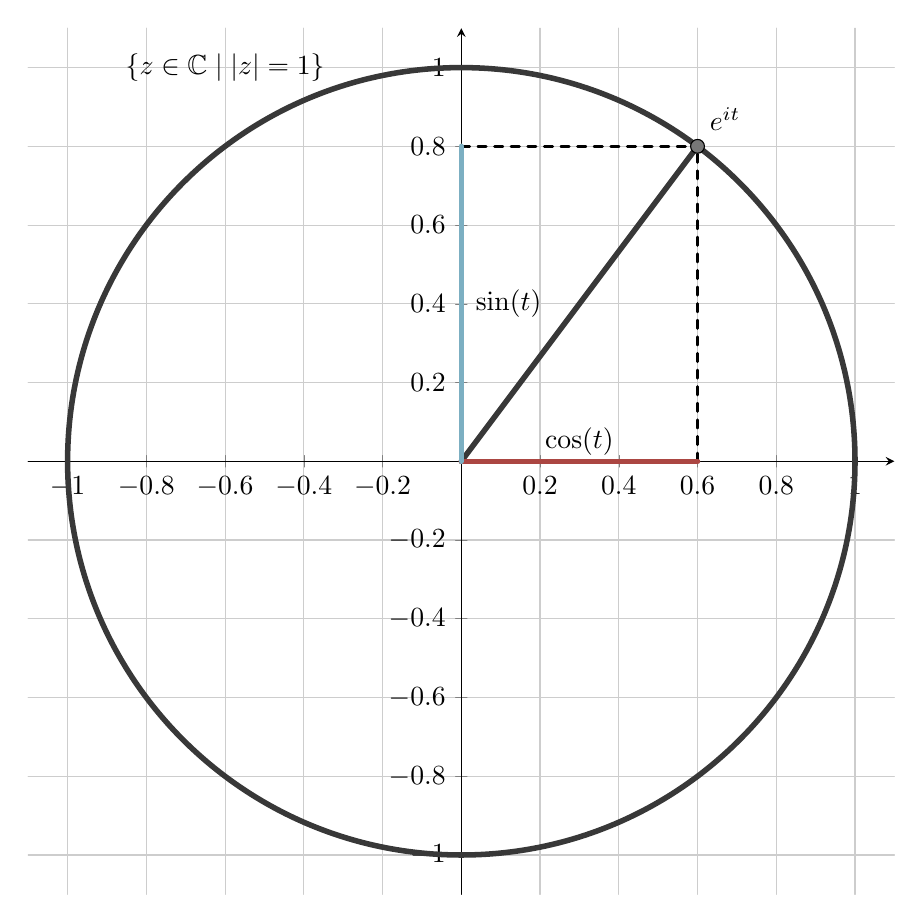
\begin{tikzpicture}[line cap=round,line join=round,>=triangle 45,x=1cm,y=1cm]
   \begin{axis}[
   x=5cm,y=5cm,
   axis lines=middle,
   ymajorgrids=true,
   xmajorgrids=true,
   xmin=-1.1, xmax=1.1,
   ymin=-1.1, ymax=1.1,
   xtick={-1,-0.8,...,1},
   ytick={-1,-0.8,...,1},]

   \draw [line width=2pt,color=black] (0,0) circle (5cm);

   \draw [line width=2pt, color=black] (0,0)-- (0.6,0.8);

   \draw [line width=1pt, dashed]  (0.6,0)-- (0.6,0.8);
   \draw [line width=1pt, dashed] (0,0.8)-- (0.6,0.8);

   \draw [line width=2pt,color=red] (0,0)-- (0.6,0);
   \draw [line width=2pt,color=blue] (0,0)-- (0,0.8);

   \draw [fill=grey] (0.6,0.8) circle (2.5pt);
   \draw (0.67, 0.87 ) node {\(e^{it}\)};
   \draw (-0.6, 1) node {\(\{z \in \mathbb{C} \mid |z| = 1\}\)};

   \draw (0.3, 0.05) node {\(\cos(t)\)};
   \draw (0.12, 0.4) node {\(\sin(t)\)};
   \end{axis}
\end{tikzpicture}

   \end{center}

   \section{Differential Calculus}
   \subsection{Definition \& Basic Properties}
   \begin{definition}[Derivative]
      \(f: (a;b) \to \mathbb{R}\) is differentiable at \(x_0 \in (a; b)\) if
      \[\frac{df}{dx} (x_0) = f'(x_0) := \lim_{h \to 0} \frac{f(x_0 + h) - f(x_0)}{h} = \lim_{x \to x_0} \frac{f(x) - f(x_0)}{x - x_0}\]
      exists.
   \end{definition}
   \begin{remark}
      We call \(f'(x_0)\) the \textit{derivative} of \(f\) at \(x_0\).
      \(f\) is differentiable on \((a; b)\) if \(\forall x_0 \in (a;b): f~\text{is differentiable at}~x_0\).
   \end{remark}
   \begin{remark}
      When we differentiate a function \(f\) we want to calculate the slope of \(f\) at \(x_0\), which is the tangent to the function graph at \(x_0\).
      To do this we start of by calculating the slope of the secant from \(\big(x_0, f(x_0)\big)\) to \(\big(x_0 + h, f(x_0) + h\big)\) through.
      \[\frac{f(x_0 + h) - f(x_0)}{h}\]
      Then we let \(h \to 0\) which makes the point \(\big(x_0 + h, f(x_0) + h\big)\) move along the function graph until it coincides with \(\big(x_0, f(x_0)\big)\).
      At this point the secant coincides (never but close enough) the tangent, then the fraction above gives us the slope of the tangent.
   \end{remark}
   \begin{remark}[Differential]
      Given a function \(y = f(x)\) we call \(dy\) and \(dx\) differentials and the relationship between them is given by
      \[dy = f'(x)dx\]
      Note that if we are just given \(f(x)\) then the differentials are \(df\) and \(dx\) and we compute them in the same manner.
      \[df = f'(x)dx \implies f'(x) = \frac{df}{dx}\]
   \end{remark}
   % TODO: add for vector space?

   \begin{center}
      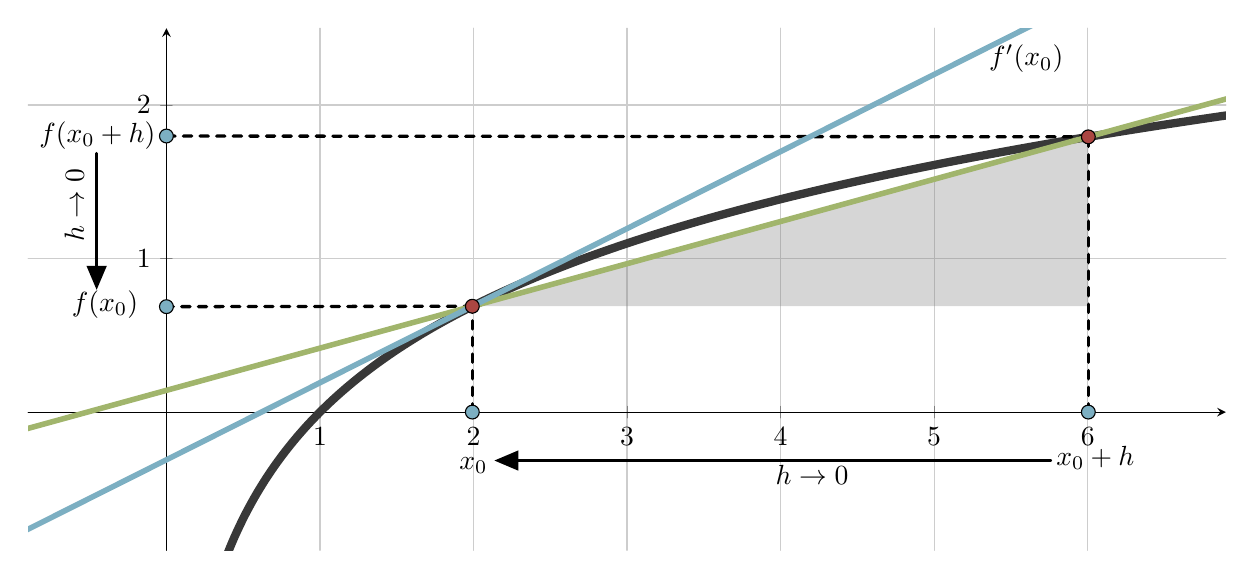
\begin{tikzpicture}[line cap=round,line join=round,>=triangle 45,x=1cm,y=1cm]
   \begin{axis}[
   x=1.95cm,y=1.95cm,
   axis lines=middle,
   ymajorgrids=true,
   xmajorgrids=true,
   xmin=-0.9, xmax=6.9,
   ymin=-0.9, ymax=2.5,
   xtick={-1,0,...,9},
   ytick={-1,0,...,5},]

      \fill[line width=2pt,color=grey,fill=grey,fill opacity=0.3] (1.992250618110671,0.689264963553256) -- (6.004283509389274,1.792473132741205) -- (6.0042835093893,0.6892649635533) -- cycle;

      \draw[line width=3pt,color=black,smooth,samples=100,domain=0.3:7] plot(\x,{ln((\x))});

      \draw [line width=1.2pt,dashed] (6.004283509389274,1.792473132741205)-- (0,1.7979325541006292);
      \draw [line width=1.2pt,dashed] (1.992250618110671,0.689264963553256)-- (0,0.6865550452377207);
      \draw [line width=1.2pt,dashed] (1.9922506,0)-- (1.992250618110671,0.689264963553256);
      \draw [line width=1.2pt,dashed] (6.0042835093893,0)-- (6.004283509389274,1.792473132741205);

      \draw [line width=2pt,color=green,domain=-2.7782759088017714:9.763751218410293] plot(\x,{(--0.5674865476121775--1.103208169187949*\x)/4.0120328912786025});
      \draw [line width=2pt,color=blue,domain=-2.7782759088017714:9.763751218410293] plot(\x,{(-0.31073503644674405--0.5019448812862405*\x)/1});
      \draw (5.6, 2.3) node {\(f'(x_0)\)};

      \draw [->,line width=1pt] (5.76,-0.3156320939175) -- (2.1362418130313,-0.3156320939175);
      \draw [->,line width=1pt] (-0.4544428683875,1.6857552136163) -- (-0.4544428683875,0.7962497436013);

      \draw [fill=blue] (0, 1.7979325541006292) circle (2.5pt);
      \draw (-0.45, 1.8) node {\(f(x_0 + h)\)};
      \draw [fill=blue] (0,0.6865550452377207) circle (2.5pt);
      \draw (-0.4, 0.7) node {\(f(x_0)\)};

      \draw [fill=blue] (1.9922506,0) circle (2.5pt);
      \draw (2, -0.35) node {\(x_0\)};
      \draw [fill=blue] (6.0042835093893,0) circle (2.5pt);
      \draw (6.050065881097502,-0.3) node {\(x_0 + h\)};

      \draw [fill=red] (1.992250618110671, 0.689264963553256) circle (2.5pt);
      \draw [fill=red] (6.004283509389274,1.792473132741205) circle (2.5pt);
      \draw (4.204342030816293,-0.4101420501065896) node {\(h \to 0\)};
      \draw (-0.6, 1.346631253173085) node {\rotatebox{90}{\(h \to 0\)}};
   \end{axis}
\end{tikzpicture}

   \end{center}

   \begin{proposition}[Derivative \(\implies\) Continuity]\label{pro:deri_impl_cont}
      If \(f: (a; b) \to \mathbb{R}\) is differentiable at \(x_0 \in (a; b)\) then is \(f\) also continuous at \(x_0\).
   \end{proposition}

   \begin{theorem}[Calculation Rules for Derivatives]\label{thm:calc_rules_deriv}
      Let \(f, g: (a; b) \to \mathbb{R}\) be differentiable at \(x_0 \in (a; b)\), then holds
      \begin{enumerate}[label=\roman*, align=Center]
         \item \((f + g)'(x_0) = f'(x_0) + g'(x_0)\)
         \item \((f \cdot g)')(x_0) = f'(x_0) \cdot g(x_0) + f(x_0) \cdot g'(x_0)\)
         \item If \(g(x_0) \neq 0\) then
            \[\left(\frac{f}{g}\right)'(x_0) = \frac{f'(x_0)\cdot g(x_0) - f(x_0) \cdot g'(x_0)}{g(x_0)^2}\]
      \end{enumerate}
   \end{theorem}

   \begin{example}[Constant Function]
      Let \(f(x) = c\) then is
      \[f'(x) = 0\]
   \end{example}
   \begin{example}[Linear Function]
      Let \(f(x) = x\) then is
      \[f'(x) = \lim_{h \to 0} \frac{f(x + h) - f(x)}{h} = \lim_{h \to 0} \frac{x + h - x}{h} = 1\]
   \end{example}
   \begin{example}
      Let \(f(x) = x^n\), then is

      \textit{IH:} \(f'(x) = n \cdot x^{n-1}\)

      \textit{IB:} \(n = 1 \implies f(x) = x \implies f'(x) = 1 \cdot x^0 = 1\)

      \textit{IS:}
      \[\frac{d}{dx} x^{n + 1} = \frac{d}{dx} x \cdot x^n = 1 \cdot x^n + x \cdot \frac{d}{dx} x^n = x^n + n \cdot x^n = (n + 1) \cdot x^n\]
   \end{example}
   \begin{remark}
      \[(a^x)' = a^x \cdot \log(a)\]
      From \cref{thm:calc_rules_deriv} follows that polynomials are always differentiable over \(\mathbb{R}\) and that rational functions are everywhere differentiable where their denominator is not 0.
   \end{remark}
   \begin{example}
      Let \(f(x) = x^{-n} = \frac{1}{x^n}\), then is
      \[f'(x) = \frac{d}{dx}x^{-n} = \frac{d}{dx} \frac{1}{x^n} = \frac{-n \cdot x^{n-1}}{x^{2n}} = -\frac{n}{x^{n+1}} = -n \cdot x^{-n - 1}\]
   \end{example}
   \begin{example}[Exponential]
      Let \(f(x) = \exp(x)\), then is
      \[\lim_{h \to 0} \frac{\exp(x + h) - \exp(x)}{h} = \lim_{h \to 0} \exp(x) \cdot \frac{\exp(h) - 1}{h} = \exp(x)\]
      because
      \[\frac{e^h - 1}{h} = \sum_{n=1}^\infty \frac{h^{n-1}}{n!} = \sum_{n = 0}^\infty \frac{h^n}{(n+1)!}\]
      The power series \(\sum \frac{h^n}{(n+1)!}\) converges on \(|h| \leq 1\) uniformly and because of that is continuous as uniform limit of continuous functions, which means that
      \[\lim_{h \to 0} \frac{e^h - 1}{h} = \lim_{h \to 0} \sum_{n=0}^\infty \frac{h^n}{(n+1)!} = 1\]
      which shows the first statement.
   \end{example}

   \begin{example}[Logarithm]
      Let \(f(x) = \log(x)\) for \(x > 0\), then is \(f\) differentiable on \((0; \infty)\)
      \[f'(x) = \frac{1}{x}\]
      To prove this we note first that
      \[\lim_{x \to 1} \frac{\log(x)}{x - 1} = 1\]
      because \(z = \log(x) \implies x = e^x\).
      Since \(\log(x)\) is continuous at 1, holds that
      \[\lim_{x \to 1} \frac{\log(x)}{x - 1} = \lim_{z \to 0} \frac{z}{e^z - 1} = \frac{1}{\lim_{z \to 0} \frac{e^z -1}{z}} = 1\]
      and so
      \[\lim_{h \to 0} \frac{\log(x + h) - \log(x)}{h} = \lim_{h \to 0} \frac{\log(1 + \frac{h}{x})}{h} = \frac{1}{x} \lim_{h \to 0} \frac{\log(1 + \frac{h}{x})}{\frac{h}{x}} = \frac{1}{x}\]
   \end{example}
   \begin{remark} %TODO: exp trick
      \[\log_a(x) = \frac{1}{x \cdot \log(a)}\]
   \end{remark}

   \begin{example}[Sine]
      Let \(f(x) = \sin(x)\), then is
      \[f'(x) = \cos(x)\]
      \[\lim_{h \to 0} \sin(h) = \lim_{h \to 0} \frac{e^{ih} - 1}{ih} = 1\]
      \begin{equation*}
         \begin{split}
            \lim_{h \to 0} \frac{\sin(x + h) - \sin(x)}{h} & = \lim_{h \to 0} \frac{e^{i(x + h)} - e^{-i(x+h)} - e^{ix} + e^{-ix}}{2ih} = \lim_{h \to 0} \frac{e^{i(x+h)} - e^{ix}}{2ih} - \lim_{h\to 0} \frac{e^{-i(x+h)} - e^{ix}}{2ih}\\
                                                           & = \frac{e^{ix}}{2} \lim_{h \to 0} \frac{e^{ih} -1}{ih} - \frac{e^{-ix}}{2} \lim_{h \to 0} \frac{e^{-ih} - 1}{ih} = \frac{e^{ix} + e^{-ix}}{2} = \cos(x)
         \end{split}
      \end{equation*}
   \end{example}

   \begin{example}[Cosine]
      Let \(f(x) = \cos(x)\), then is
      \[f'(x) = -\sin(x)\]
      This can be proven similar as for \(\sin\) above.
      \Cref{thm:calc_rules_deriv} implies that \(\tan(x)\) is differentiable at \(\forall x \neq (n + \frac{1}{2})\pi\) for some \(n \in \mathbb{Z}\).
   \end{example}

   \begin{proposition}\label{pro:deriv_cont}
      Let \(x_0 \in (a;b)\).
      \(f: (a;b) \to \mathbb{R}\) is differentiable at \(x_0\) iff \(\exists k: (a;b) \to \mathbb{R}\) which is continuous at \(x_0\) and where
      \[\forall x \in (a;b): f(x) = f(x_0) + k(x) \cdot (x - x_0)~\text{then holds that} \quad k(x_0) = f'(x_0)\]
   \end{proposition}

   \begin{proposition}[Chain Rule for Derivatives]\label{pro:chain_rule}
      Let \(x_0 \in (a;b)\) and \(f: (a;b) \to \mathbb{R}\) differentiable at \(x_0\).
      Further let \(y_0 = f(x_0) \in (c;d)\) and \(g: (c;d) \to \mathbb{R}\) be differentiable at \(y_0\), then is \(g \circ f\) differentiable at \(x_0\) and
      \[(g(f(x))' = g'(f(x_0)) \cdot f'(x_0)\]
   \end{proposition}
   \begin{example}
      Let \(f(x) = x^\alpha = \exp(\alpha \log(x))\) defined for some \(\alpha \in \mathbb{R}\) and \(x \in (0;\infty)\).
      \[\frac{d}{dx}x^\alpha = \exp(\alpha \log(x)) \cdot \alpha \cdot \frac{1}{x} = \alpha \cdot x^{\alpha -1}\]
   \end{example}
   \begin{example}
      Let \(f(x) = x^x = \exp(x \log(x))\)
      \[\frac{d}{dx}x^x = \exp(x \log(x)) (\log(x) + x \cdot \frac{1}{x}) = x^x (\log(x) + 1)\]
   \end{example}

   \begin{proposition}[Differentiable Inverse]\label{pro:diff_inv}
      Let \(x_0 \in (a;b)\) and \(f: (a;b) \to \mathbb{R}\) continuous, strictly monotonic and differentiable at \(x_0\) with \(f'(x_0) \neq 0\), then is

      \(f^{-1}\) differentiable at \(x_0\) with
      \[(f^{-1})'(f(x_0)) = \frac{1}{f'(x_0)}\]
   \end{proposition}
   \begin{remark}
      If \(f\) is increasing \(f^{-1}\) is defined on \(\big(f(a), f(b)\big)\) if \(f\) is decreasing on \(\big(f(b); f(a)\big)\).
   \end{remark}
   \begin{example}
      \(\exp: \mathbb{R} \to (0; \infty)\) is strictly increasing and differentiable and its inverse is \(\log: (0; \infty) \to \mathbb{R}\).
      From the proposition follows that \(\log\) is differentiable on \((0; \infty)\) and
      \[\forall x \in \mathbb{R}: \log'(\exp(x)) = \frac{1}{\exp(x)} \implies \log'(y) = \frac{1}{y}\]
   \end{example}
   \begin{example}
      Let \(f(x) = \tan(x): \left(-\frac{\pi}{2}; \frac{\pi}{2}\right) \to \mathbb{R}\).
      \(f\) is strictly increasing and differentiable
      \begin{equation*}
         \begin{split}
            f'(x) & = \frac{d}{dx} \left(\frac{\sin(x)}{\cos(x)}\right) = \frac{\sin'(x)\cos(x) - \sin(x)\cos'(x)}{\cos(x)^2} = \frac{\cos(x)\cos(x) - \sin(x)(-\sin(x))}{\cos(x)^2}\\
                  & = \frac{\cos(x)^2}{\cos(x)^2} + \frac{\sin(x)^2}{\cos(x)^2} = 1 + \tan(x)^2
         \end{split}
      \end{equation*}
      Its inverse is \(\arctan: \mathbb{R} \to \left(-\frac{\pi}{2}; \frac{\pi}{2}\right)\) and for arbitrary \(x \in \mathbb{R}\) and \(y \in \left(-\frac{\pi}{2}; \frac{\pi}{2}\right)\) holds
      \[\arctan'(\tan(x)) = \frac{1}{1 + \tan(x)^2} \implies \arctan'(y) = \frac{1}{1 + y^2}\]
   \end{example}

   \begin{example}[Recipe]
      We regard
      \[g(x) := \begin{cases}f(x) & x \neq x_0\\g(x_0)\end{cases}\]
      We want to know if
      \begin{enumerate}
         \item \(g\) is continuous
            \begin{enumerate}%TODO
               \item \(f\) continuous in \(x \neq x_0\)? If so we can use common rules.
               \item \(\lim_{x \to x_0} f(x) = g(x)\)? If so, then is \(g\) continuous.
            \end{enumerate}
         \item \(g\) is differentiable
            \begin{enumerate}
               \item \(f\) differentiable in \(x \neq x_0\)? If so we can use derivative rules.
               \item \(g'(x_0) := \lim_{h \to 0} \frac{f(x_0 + h) - g(x_0)}{h}\) exists? If so, then is \(g\) differentiable.
            \end{enumerate}
         \item \(g\) is continuously differentiable (\(g \in C^1\))
            \begin{enumerate}
               \item \(f'\) continuous in \(x \neq x_0\)?
               \item \(\lim_{x \to x_0} f'(x) = g'(x_0)\)? If so, then is \(g'\) continuous.
            \end{enumerate}
      \end{enumerate}
   \end{example}

   \subsection{Derivative \& Optimization}
   \begin{definition}[Global Extremum of a Function]
      Given \(f: I \to \mathbb{R}\). \(x_0 \in I\) is a global
      \[\text{maximum} :\iff \forall x \in I: f(x) \leq f(x_0)\]
      \[\text{minimum} :\iff \forall x \in I: f(x_0) \leq f(x)\]
   \end{definition}

   Finding global maxima and minima is the goal of mathematical optimization.
   If a function is continuous on a closed interval, then by the extreme value theorem (\ref{thm:extreme_value}) global maxima and minima exist.
   Furthermore, a global maximum must be a local maximum and can be characterized by \(f'(x) = 0\) (since if \(f'(x) \neq 0\) we can still move in one or the other direction to keep ascending).
   It's also possible that the maxima lay on a point where \(f\) is not differentiable.

   \begin{definition}[Local Extremum of a Function]
      Given \(f: I \to \mathbb{R}\). \(x_0 \in I\) is a local
      \[\text{maximum} :\iff \exists \varepsilon > 0: \big(\forall x \in (x_0 - \varepsilon; x_0 + \varepsilon): f(x) \leq f(x_0)\big)\]
      \[\text{minimum} :\iff \exists \varepsilon > 0: \big(\forall x \in (x_0 - \varepsilon; x_0 + \varepsilon): f(x_0) \leq f(x)\big)\]
   \end{definition}
   \begin{remark}
      We say \(f\) is locally \textit{extremal} at \(x_0\) if \(f\) is locally minimal or maximal at \(x_0\).
   \end{remark}

   \begin{proposition}[Derivative \(\neq 0 \implies\) Not Extrema]\label{pro:diff=0_not_extreme}
      Let \(x_0 \in (a;b)\) and \(f: (a;b) \to \mathbb{R}\) be differentiable at \(x_0\) with \(f'(x_0) \neq 0\), then is \(f\) not extremal at \(x_0\).
   \end{proposition}
   \begin{example}
      Which rectangle with circumference \(p\) has the largest area?
      Let \(x, y\) be the two side lengths hence \(p = 2 (x + y)\) for which (naturally) must hold
      \[0 \leq x, y \leq \frac{p}{2}\]
      The surface area is \(A = x \cdot y\) and with \(p = 2 (x + y) \implies y = \frac{p}{2} - x\) follows \(A = x \cdot y = x \cdot \left(\frac{p}{2} - x\right)\).
      To make \(A\) maximal we regard it as a function, respecting the restrictions above
      \[A: \left[0; \frac{p}{2}\right] \to \mathbb{R}~\text{where}~A(x) := x \cdot \left(\frac{p}{2} - x\right)~\text{and so}~A'(x) = \frac{p}{2} - 2x\]
      so we see that \(A'(x) = 0 \iff x = \frac{p}{4}\) hence is \(A\) maximal if
      \[A\left(\frac{p}{4}\right) = \frac{p^2}{16}\]
      which means that \(A\) is maximal if the rectangle is a square.
   \end{example}

   \subsection{Mean Value Theorem}
   \begin{theorem}[Rolle's Theorem]\label{thm:rolles_thm}
      Let \(f: [a; b] \to \mathbb{R}\) be continuous and differentiable on \((a; b)\) and \(f(a) = f(b)\), then
      \[\exists \xi \in (a; b): f'(\xi) = 0\]
   \end{theorem}

   \begin{center}
      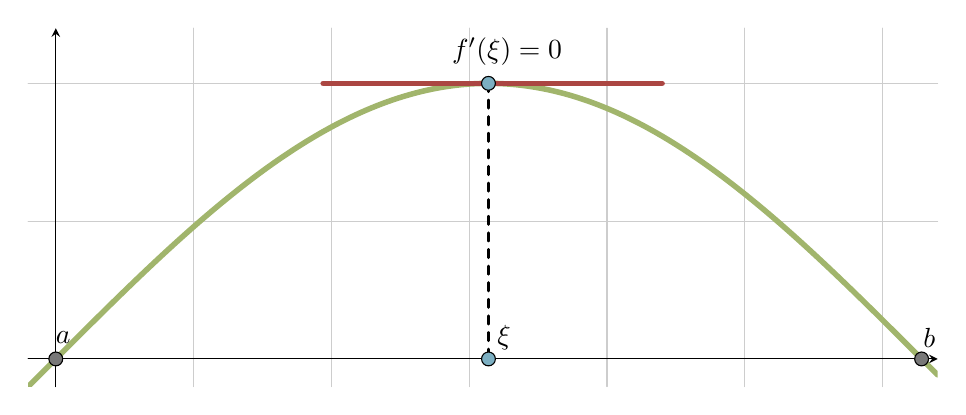
\begin{tikzpicture}[line cap=round,line join=round,>=triangle 45,x=1cm,y=1cm]
   \begin{axis}[
   ticks=none,
   x=3.5cm,y=3.5cm,
   axis lines=middle,
   ymajorgrids=true,
   xmajorgrids=true,
   xmin=-0.1, xmax=3.2,
   ymin=-0.1, ymax=1.2,]

   \draw [line width=2pt,color=green,smooth,samples=100,domain=-0.1:3.2] plot(\x,{sin(((\x))*180/pi)});
   \draw [line width=2pt,color=red] (2.2,1)-- (0.9702955586506,1);
   \draw [line width=1pt,dashed] (1.57,1)-- (1.57,0);

   \draw [fill=blue] (1.57,0.9999996829318346) circle (2.5pt);
   \draw (1.6374360725194987,1.115793406601803) node {\(f'(\xi) = 0\)};

   \draw [fill=blue] (1.57,0) circle (2.5pt);
   \draw (1.6268423841076651,0.07761194224209192) node {\(\xi\)};
   \draw [fill=grey] (0,0) circle (2.5pt);
   \draw (0.027195433920788957,0.07761194224209192) node {\(a\)};
   \draw [fill=grey] (3.1415926548458097,-1.2560165015758325E-9) circle (2.5pt);
   \draw (3.169989662764762,0.07761194224209192) node {\(b\)};
   \end{axis}
\end{tikzpicture}

   \end{center}

   \begin{theorem}[Mean Value Theorem]\label{thm:mean_value}
      Let \(f: [a; b] \to \mathbb{R}\) be continuous and differentiable on \((a; b)\), then
      \[\exists \xi \in (a; b): f'(\xi) = \frac{f(b) - f(a)}{b - a}\]
   \end{theorem}

   \begin{center}
      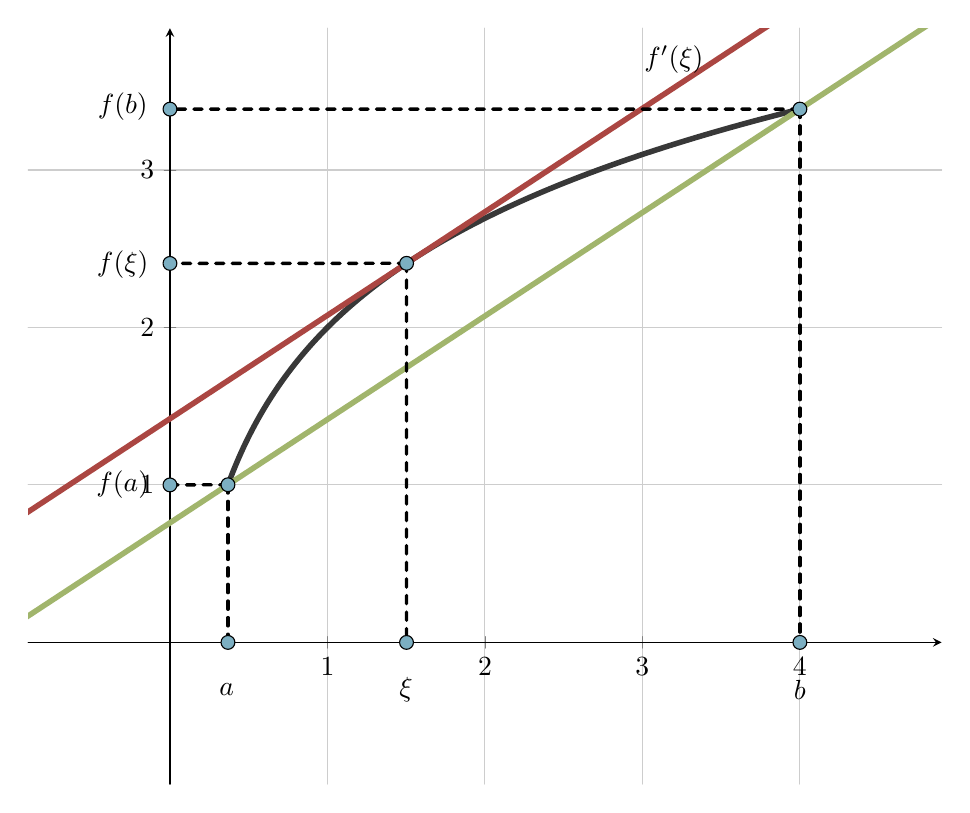
\begin{tikzpicture}[line cap=round,line join=round,>=triangle 45,x=1cm,y=1cm]
   \begin{axis}[
   x=2cm,y=2cm,
   axis lines=middle,
   ymajorgrids=true,
   xmajorgrids=true,
   xmin=-0.9, xmax=4.9,
   ymin=-0.9, ymax=3.9,
   xtick={-1,0,...,8},
   ytick={-1,0,...,5},]

      \draw[line width=2pt,color=black,smooth,samples=100,domain=0.36:4] plot(\x,{ln((\x))+2});

      \draw [line width=2pt,color=green,domain=-2:5] plot(\x,{(--2.7573527493500425--2.385168241636624*\x)/3.6317060492725224});
      \draw [line width=2pt,color=red,domain=-2:5] plot(\x,{(--5.158273859205579--2.385168241636624*\x)/3.6317060492725224});

      \draw [line width=1.2pt, dashed] (0.3682939507274774,1.0011261194832666)-- (0.3682939507274774,0);
      \draw [line width=1.2pt, dashed] (4,3.386294361119891)-- (4,0);
      \draw [line width=1.2pt, dashed] (1.502473495262215,2.407112746847149)-- (1.5020554512845232,0);
      \draw [line width=1.2pt, dashed] (0.3682939507274774,1.0011261194832666)-- (0,1);
      \draw [line width=1.2pt, dashed] (1.502473495262215,2.407112746847149)-- (0,2.4065499918014557);
      \draw [line width=1.2pt, dashed] (4,3.386294361119891)-- (0,3.386267787117416);

      \draw [fill=blue] (0.3682939507274774,1.0011261194832666) circle (2.5pt);
      \draw [fill=blue] (4,3.386294361119891) circle (2.5pt);
      \draw [fill=blue] (1.502473495262215,2.407112746847149) circle (2.5pt);

      \draw (3.2, 3.7) node {\(f'(\xi)\)};

      \draw [fill=blue] (0.3682939507274774,0) circle (2.5pt);
      \draw (0.36, -0.3) node {\(a\)};
      \draw [fill=blue] (1.5020554512845232,0) circle (2.5pt);
      \draw (1.5, -0.3) node {\(\xi\)};
      \draw [fill=blue] (4,0) circle (2.5pt);
      \draw (4, -0.3) node {\(b\)};

      \draw [fill=blue] (0,1) circle (2.5pt);
      \draw (-0.3, 1) node {\(f(a)\)};
      \draw [fill=blue] (0,2.4065499918014557) circle (2.5pt);
      \draw (-0.3, 2.4) node {\(f(\xi)\)};
      \draw [fill=blue] (0,3.386267787117416) circle (2.5pt);
      \draw (-0.3, 3.4) node {\(f(b)\)};
   \end{axis}
\end{tikzpicture}

   \end{center}

   \begin{theorem}[Cauchy's Mean Value Theorem]\label{thm:extended_mean_value}
      Let \(f, g: [a; b] \to \mathbb{R}\) be continuous and differentiable on \((a; b)\) with \(\forall x \in (a; b): g'(x) \neq 0\), then
      \[\exists \xi \in (a; b): \frac{f'(\xi)}{g'(\xi)} = \frac{f(b) - f(a)}{g(b) - g(a)}\]
   \end{theorem}

   \begin{remark}
      The mean value theorems do not hold for \(f\) with values in \(\mathbb{R}^m\) or \(\mathbb{C}\).
      We can however use an estimation.
   \end{remark}

   \begin{proposition}[Mean Value Estimation]\label{pro:mean_value_estim}
      Let \(f: [a; b] \to \mathbb{R}^m\) be continuous and differentiable on \((a; b)\) with \(\forall x \in (a; b): \|f'(x)\| \leq M\) then holds
      \[\|f(b) - f(a)\| \leq M \cdot |b - a|\]
   \end{proposition}

   \begin{corollary}\label{cor:mean_value_estim}
      Let \(f: [a; b] \to \mathbb{R}^m\) be continuous with \(\forall x \in (a; b): f'(x) = 0\), then is \(f\) constant on \([a; b]\).
   \end{corollary}

   \begin{proposition}[Monotonicity Criterion for Derivatives]\label{pro:pos_derivative=increasing}
      Let \(f: [a; b] \to \mathbb{R}\) continuous and differentiable on \((a; b)\), then is
      \[f~\text{increasing on}~[a;b] \iff \forall x \in (a; b): f'(x) \geq 0\]
      \[f~\text{decreasing on}~[a;b] \iff \forall x \in (a; b): f'(x) \leq 0\]
   \end{proposition}
   \begin{remark}
      Keep in mind however that only \(\forall x \in (a; b): f'(x) > 0 \implies f~\text{strictly increasing}\).
   \end{remark}
   \begin{example}
      Let \(f(x) = x^3\).
      This example shows that \(f\) can be strictly increasing even though \(\exists x: f'(x) = 0\) (in this case \(f'(0) = 0\)).

      Now to the critical distinction when the derivative implies strict monotonicity.

      If \(f\) is increasing on \([a; b]\) then \(\exists c, d \in [a; b]: c < d\) where \(f(c) = f(d)\).
      Since \(f\) is monotonic follows that
      \[\forall x \in [c; d]: f(x) = f(c) \implies \forall x \in (c; d) f'(x) = 0\]
      This means that increasing (but not strictly increasing) functions are constant on a certain intervall, which means that the derivative disappears on said intervall.
   \end{example}

   \begin{proposition}
      Let \(f: [a;b] \to \mathbb{R}\) be continuous and differentiable on \((a; b)\), then is \(f\) strictly increasing on \([a;b]\) iff
      \[\forall x \in (a; b): f'(x) \geq 0~\text{and}~\nexists [c;d]~\text{of positive length where}~\forall x \in (c; d): f'(x) = 0\]
   \end{proposition}

   \begin{theorem}[Bernoulli--de L'H\^{o}pital]\label{thm:lhopital}
      Let \(f, g\) be differentiable on \((a; b)\) where
      \[\lim_{x \to x_0} f(x), \lim_{x \to x_0} g(x) \in \{0, \pm\infty\}~\text{then holds} \quad \lim_{x \to x_0} \frac{f(x)}{g(x)} = \lim_{x \to x_0} \frac{f'(x)}{g'(x)}\]
   \end{theorem}
   \begin{remark}
      We would actually state this theorem only for one-sided limits and if \(x \downarrow a = x \uparrow a\) we can use it for \(x \to a\).
      If \(\lim_{x \downarrow a} f(x) = \lim_{x \downarrow a} g(x) = \pm \infty\), it doesn't hold for functions with values in \(\mathbb{C}\).
   \end{remark}
   \begin{example}
      Wee see a \(\frac{0}{0}\) situation, so we apply lhopital
      \[\lim_{x \to 0} \frac{\sin(x)}{x} = \lim_{x \to 0} \frac{\cos(x)}{1} = 1\]
   \end{example}
   \begin{remark}
      It is important to remember the \(e^{\log}\) trick.
      \[\lim_{x \to x_0} f(x)^{g(x)} = \lim_{x \to x_0} e^{\log(f(x)^{g(x)})} = \lim_{x \to x_0} e^{g(x) \cdot \log(f(x))} \overset{e~\text{cont.}}{=} \exp \left(\lim_{x \to x_0} g(x) \cdot log(f(x))\right)\]
      is sometimes easier to calculate.
   \end{remark}
   \begin{example}
      \[\lim_{x \downarrow 0} x^{\sin(x)} = \exp\left(\lim_{x \downarrow 0} \sin(x) \cdot log(x)\right) = \exp\left(\lim_{x \downarrow 0} \frac{\log(x)}{\frac{1}{\sin(x)}}\right) \overset{\text{l'hop.}}{=} \exp\left(\lim_{x \downarrow 0} \frac{-\sin(x)^2}{x \cdot \cos(x)}\right) = e^0 = 1\]
   \end{example}
   \begin{example}
      We want to calculate \(\lim_{x \to 0} \frac{1}{\sin(x)} - \frac{1}{x}\).
      First we need to see that
      \[\frac{1}{\sin(x)} - \frac{1}{x} = \frac{x - \sin(x)}{x \sin(x)}\]
      so we can apply the theorem for \(f(x) := x - \sin(x)\) and \(g(x) := x \sin(x)\).
      \[\lim_{x \to 0} \frac{f(x)}{g(x)} \overset{\text{thm}}{=} \lim_{x \to 0} \frac{f'(x)}{g'(x)} = \lim_{x \to 0} \frac{1 - \cos(x)}{\sin(x) + x \cos(x)} \overset{\text{thm}}{=} \lim_{x \to 0} \frac{f''(x)}{g''(x)} = \lim_{x \to 0} \frac{\sin(x)}{2 \cos(x) - x \sin(x)} = 0\]
      since as \(x \to 0\) are \(\cos(x) \to 1\) and \(\sin(x) \to 0\).
   \end{example}

   \subsection{Higher Order Derivatives}
   \begin{definition}[n-th Derivative]
      \(f: (a; b) \to \mathbb{R}\) is \(n\) times differentiable at \(x_0 \in (a; b)\) if \(f^{(n-1)}(x)\) is defined in a neighbourhood of \(x_0\) and if \(f: x \to f^{(n-1)}(x)\) is differentiable at \(x_0\).
      \[\frac{d^n f}{dx^n} = f^{(n)} = (f^{(n-1)})'\]
   \end{definition}
   \begin{remark}
      Let \(a, b \in (-\infty; \infty): a < b\).
      \(f\) is \(n\) times differentiable on \((a; b)\) if \(\forall x \in (a; b): f~n~\text{times differentiable at}~x\).
   \end{remark}

   \begin{definition}[Continuous Derivative]
      \(f: (a; b) \to \mathbb{R}\) is \(n\) times continuously differentiable if \(f: x \to f^{(n)}(x)\) is continuous on \((a; b)\).
      \[f \in C^n\big((a; b)\big) := \{f \mid f~\text{defined, real-valued,}~n~\text{times continuously differentiable on}~(a;b)\}\]
   \end{definition}
   \begin{remark}[Notation]
      \[C^0\big((a;b)\big) = C\big((a; b)\big) \quad \text{Set of continuous functions on}~(a; b)\]
      \[C_b\big((a; b)\big) \quad \text{Set of bounded continuous functions on}~(a; b)\]
      \[C^n\big((a; b); \mathbb{C}\big) \quad \text{Set of complex-valued,}~n~\text{times continuously differentiable functions on}~(a; b)\]
   \end{remark}
   \begin{remark}
      \[(f \in C^m\big((a; b)\big) \implies f^{(m-1)}~\text{continuous}) \implies \forall 0 \leq j \leq m: f \in C^j\big((a; b)\big)\]
      \[C\big((a; b)\big) \supset C^1\big((a; b)\big) \supset \ldots \rightsquigarrow C^\infty\big((a; b)\big) = \bigcap_{n=0}^\infty C^n\big((a; b)\big)\]
      Is \(f \in C^\infty\big((a; b)\big)\) we say \(f\) is on \((a; b)\) arbitrary many times differentiable.
      \[f \in C^m\big((a; b)\big) \iff f \in C^1\big((a; b)\big) \land f' \in C^{m-1}\big((a; b)\big)\]
   \end{remark}

   \begin{proposition}\label{pro:func_add_in_Cm}
      Let \(a, b \in [-\infty; \infty]: a < b\) and \(f, g \in C^m\big((a;b)\big)\), then is
      \[f + g~\text{and}~f \cdot g \in C^m\big((a;b)\big)\]
   \end{proposition}

   \begin{proposition}\label{pro:func_comp_in_Cm}
      Let \(f \in C^m\big((a;b)\big)\), \(\im(f) \subset (c; d) \subset \mathbb{R}\) and \(g \in C^m\big((c; d)\big)\), then is
      \[g \circ f \in C^m\big((a;b)\big)\]
   \end{proposition}

   \begin{proposition}\label{pro:func_inv_in_Cm}
      Let \(f \in C^m\big((a;b)\big)\) with \(\forall x \in (a;b): f'(x) \neq 0\), then is
      \[f^{-1} \in C^m\bigg(f\big((a;b)\big)\bigg)\]
   \end{proposition}

   \subsection{Convexity}
   \begin{definition}[Convex Function]
      Given \(a, b \in [-\infty; \infty]: a < b\), \(f: (a; b) \to \mathbb{R}\) is convex if
      \[\forall x, y, \in (a; b), \lambda \in [0; 1]: f(\lambda \cdot x + (1 - \lambda) \cdot y) \leq \lambda \cdot f(x) + (1 - \lambda) \cdot f(y)\]
   \end{definition}
   \begin{remark}
      With \(<\) and \(>\) is \(f\) \textit{strictly convex}
      A function can also change its convexity.
   \end{remark}

   \begin{definition}[Concave Function]
      Given \(a, b \in [-\infty; \infty]: a < b\), \(f: (a; b) \to \mathbb{R}\) is concave if
      \[\forall x, y, \in (a; b), \lambda \in [0; 1]: \lambda \cdot f(x) + (1 - \lambda) \cdot f(y) \leq f(\lambda \cdot x + (1 - \lambda) \cdot y)\]
   \end{definition}

   \begin{center}
      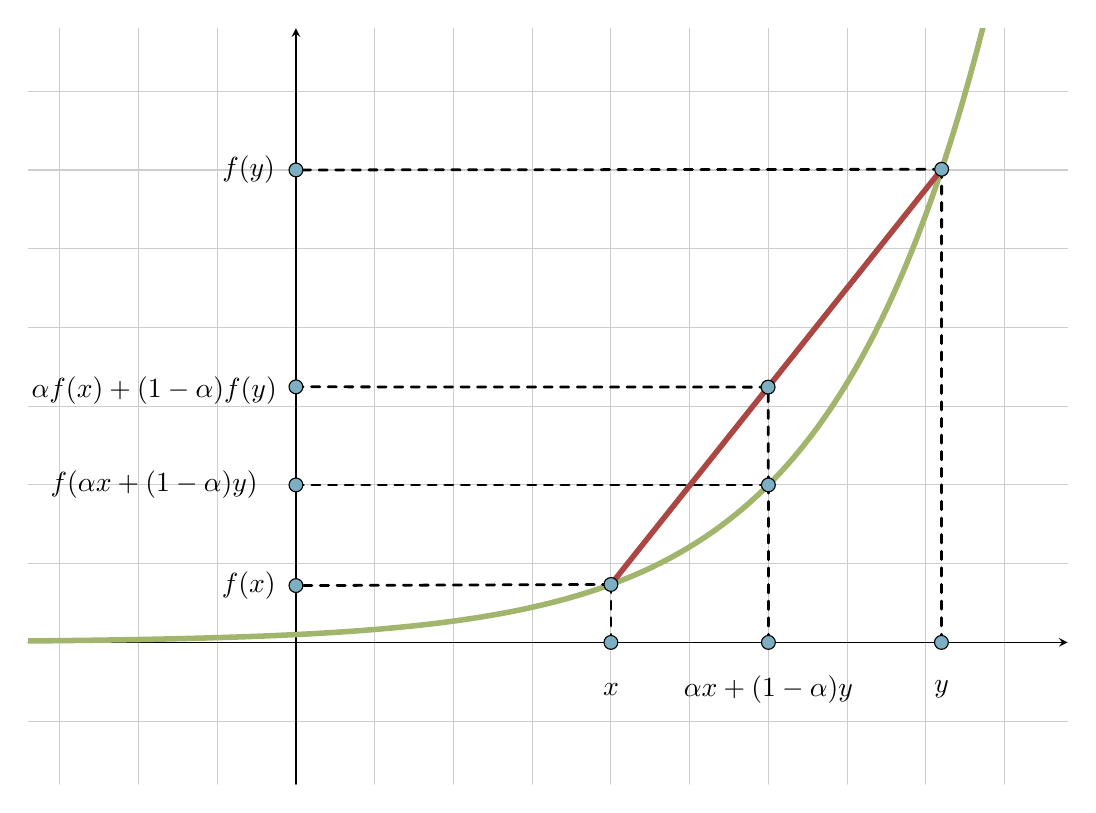
\begin{tikzpicture}[line cap=round,line join=round,>=triangle 45,x=1cm,y=1cm]
   \begin{axis}[
   ticks=none,
   x=2cm,y=2cm,
   axis lines=middle,
   ymajorgrids=true,
   xmajorgrids=true,
   xmin=-1.7, xmax=4.9,
   ymin=-0.9, ymax=3.9,]

      \draw [line width=2pt,color=green,smooth,samples=100,domain=-2:5] plot(\x,{2.71828^((\x)-(3))});

      \draw [line width=1pt,dashed] (4.100035747431382,3.0042734170847365)-- (0,3);
      \draw [line width=1pt,dashed] (4.100035747431382,3.0042734170847365)-- (4.098775396739197,0);
      \draw [line width=1pt,dashed] (2,0.36787944117144233)-- (2,0);
      \draw [line width=1pt,dashed] (2,0.36787944117144233)-- (0,0.36081515180285156);
      \draw [line width=1pt,dashed] (3,1)-- (3,0);
      \draw [line width=1pt,dashed] (3,1)-- (2.9981431045318674,1.6209526191427581);
      \draw [line width=1pt,dashed] (2.9981431045318674,1.6209526191427581)-- (0,1.622849158944273);
      \draw [line width=1pt,dashed] (3,1)-- (0,1);

      \draw [line width=2pt,color=red] (2,0.36787944117144233)-- (4.100035747431382,3.0042734170847365);

      \draw [fill=blue] (4.100035747431382,3.0042734170847365) circle (2.5pt);
      \draw [fill=blue] (2.9981431045318674,1.6209526191427581) circle (2.5pt);
      \draw [fill=blue] (3,1) circle (2.5pt);
      \draw [fill=blue] (3,0) circle (2.5pt);
      \draw [fill=blue] (2,0.36787944117144233) circle (2.5pt);

      \draw [fill=blue] (0,3) circle (2.5pt);
      \draw (-0.3,3) node {\(f(y)\)};
      \draw [fill=blue] (4.098775396739197,0) circle (2.5pt);
      \draw (4.1, -0.3) node {\(y\)};
      \draw [fill=blue] (2,0) circle (2.5pt);
      \draw (2,-0.3) node {\(x\)};
      \draw [fill=blue] (0,0.36081515180285156) circle (2.5pt);
      \draw (-0.3, 0.36) node {\(f(x)\)};
      \draw (3,-0.3) node {\(\alpha x + (1 - \alpha)y\)};
      \draw [fill=blue] (0,1.622849158944273) circle (2.5pt);
      \draw (-0.9, 1.6) node {\(\alpha f(x) + (1 - \alpha) f(y)\)};
      \draw [fill=blue] (0,1) circle (2.5pt);
      \draw (-0.9,1) node {\(f(\alpha x + (1-\alpha)y)\)};
   \end{axis}
\end{tikzpicture}

   \end{center}

   \begin{lemma}\label{lem:secant_increasing}
      Let \(f\) be convex on \((a;b)\), then is
      \[\forall x < y~\text{the slope of the secant}~m(x, y) = \frac{f(y) - f(x)}{y - x}~\text{increasing.}\]
   \end{lemma}

   \begin{proposition}[Convexity \(\implies\) Continuity]\label{pro:convex_implies_cont}
      Let \(f\) be convex on \((a; b)\) and \(x \in (a; b)\), then exist
      \[f'(x^+) := \lim_{h \downarrow 0} \frac{f(x + h) - f(x)}{h} \quad\text{and}\quad f'(x^-) := \lim_{h \uparrow 0} \frac{f(x + h) - f(x)}{h}\]
      \(f\) is continuous at \(x\) and \(f'(x^-) \leq f'(x^+)\).
      Furthermore for \(x, y \in (a; b): x < y\) holds
      \[f'(x^+) \leq \frac{f(y) - f(x)}{y - x} \leq f'(y^-)\]
   \end{proposition}
   \begin{remark}
      % TODO: graphic
      This proposition basically states that the slope \(f'(x^+)\) is smaller than the secant which is smaller than the slope \(f'(x^-)\).
   \end{remark}

   \begin{proposition}[Second Derivative shows Convexity]\label{pro:second_deriv_convex}
      Let \(f\) be differentiable on \((a; b)\), then is
      \begin{enumerate}[label=\roman*, align=Center]
         \item \(f~\text{convex} \iff f'~\text{increasing on}~(a;b)\)
         \item \(f~\text{concave} \iff f'~\text{decreasing on}~(a;b)\)
         \item If \(f'\) is differentiable, then is\\
            \(f~\text{convex} \iff \forall x \in (a; b): f'' \geq 0\)\\
            \(f~\text{concave} \iff \forall x \in (a; b): f'' \leq 0\)
      \end{enumerate}
   \end{proposition}
   \begin{remark}
      The second derivative measure whether \(f\) is convex or concave.
      \(f'' > 0 \implies f~\text{strictly convex}\).
      \(f'' < 0 \implies f~\text{strictly concave}\).
   \end{remark}

   \begin{definition}[Support Function]
      Given a convex function \(f: (a; b) \to \mathbb{R}\) and \(x_0 \in (a; b)\).
      \[\phi(x) := \phi(x_0) + m(x - x_0) \quad\text{with}\quad \phi(x_0) = f(x_0)\]
      is a support function of \(f\) which is entirely beneath \(f\): \(\forall x \in (a;b): \phi(x) \leq f(x)\).
   \end{definition}

   \begin{proposition}\label{pro:support_func}
      Let \(f\) be convex on an intervall \(I\), \(x_0 \in I^\circ\) and \(\overline{m} \in \mathbb{R}\) where \(f'(x_0^-) \leq \overline{m} \leq f'(x_0^+)\), then is
      \[\phi(x) = f(x_0) + \overline{m}(x - x_0)\]
      a support function of \(f\) at \(x_0\).
   \end{proposition}
   \begin{remark}
      If \(f\) is differentiable at \(x_0\) then is the tangent with the slope \(f'(x_0)\) the only support function.
   \end{remark}

   \begin{proposition}[Jensen's Inequality]\label{pro:jensen_ineq}
      Let \(f\) be convex on \((a; b)\), \(x_1, \ldots, x_n \in (a; b)\) and \(\lambda_1, \ldots, \lambda_n \in [0; 1]: \sum_{i = 1}^n \lambda_i = 1\), then is
      \[f\left(\sum_{i=1}^n \lambda_i x_i\right) \leq \sum_{i=1}^n \lambda_i f(x_i)\]
   \end{proposition}
   \begin{remark}
      For \(n = 2\) we get the definition of convexity.

      If \(f\) is strictly convex and there are at least two indices \(i \neq j\) with \(\lambda_i, \lambda_j \neq 0\) and \(x_i \neq x_j\) then holds
      \[f\left(\sum_{i=1}^n \lambda_i x_i\right) < \sum_{i = 1}^n \lambda_i f(x_i)\]
   \end{remark}
   \begin{proof}
      We prove this by induction over \(n\).

      \textit{IB:} For \(n = 2\) is the statement the definition of convexity.

      \textit{IH:} Suppose the inequality holds for some \(n \in \mathbb{N}\).

      \textit{IS:} We can assume that \(\lambda_{n+1} \neq 0, 1\) since those cases are trivial.
      \begin{equation*}
         \begin{split}
            f\left(\sum_{i=1}^{n+1} \lambda_i x_i\right) & = f\left(\sum_{i=1}^n \lambda_i x_i + \lambda_{n+1} x_{n+1}\right)\\
                                                         & = f\left(\sum_{i=1}^n\left(\frac{1- \lambda_{n+1}}{1 - \lambda_{n+1}}\right) \lambda_i x_i + \lambda_{n+1} x_{n+1}\right) - f\left((1 - \lambda_{n+1})\sum_{i=1}^n \frac{\lambda_i}{1-\lambda_{n+1}}x_i + \lambda_{n+1}x_{n+1}\right)\\
                                                         & \overset{\text{convex.}}{\leq} (1 - \lambda_{n+1}) f\left(\sum_{i=1}^n \frac{\lambda_i}{1 - \lambda_{n+1}} x_i\right) + \lambda_{n+1} f(x_{n+1})\\
                                                         & \overset{\text{IH}}{\leq} (1 - \lambda_{n+1}) \sum_{i=1}^n \frac{\lambda_i}{1 - \lambda_{n+1}} f(x_i) + \lambda_{n+1}f(x_{n+1})\\
                                                         & = \sum_{i=1}^n \lambda_i f(x_i) + \lambda_{n+1}f(x_{n+1}) = \sum_{i=1}^{n+1} \lambda_i f(x_i)
         \end{split}
      \end{equation*}
   \end{proof}

   \subsection{Taylor Polynomials}
   \begin{definition}[Taylor Polynomial]
      Given \(f \in C^{n-1}\big([a;b]\big)\) n times differentiable where \(n > 1\), the \textit{n}th order taylor polynomial at \(x_0\) is
      \[T_{x_0}^n f(x) := \sum_{k=0}^n \frac{f^{(k)}(x_0)}{k!} (x - x_0)^k\]
   \end{definition}
   \begin{remark}
      \[T_{x_0}^n f(x) = f(x_0) + \frac{f'(x_0)}{1!}(x - x_0)^1 + \frac{f''(x_0)}{2!}(x-x_0)^2 + \ldots + \frac{f^{(n)}(x_0)}{n!} (x-x_0)^n\]
   \end{remark}

   \begin{theorem}[Lagrange Error Estimation]\label{thm:talyor_approx}
      Let \(f \in C^{n}\big([a; b]\big)\) be \(n+1\) times differentiable on \((a; b)\) and \(x_0 \in (a; b)\), then
      \[\forall x \in (a;b)~\exists \xi \in (x_0; x): R_{x_0}^n f(x) := f(x) - T_{x_0}^n f(x) = \frac{f^{(n+1)}(\xi)}{(n+1)!} (x - x_0)^{n+1}\]
   \end{theorem}
   \begin{remark}
      It is important to note that \(\xi\) depends on \(x\).
   \end{remark}
   \begin{remark}
      The approximation works since \((x - a)^m \xrightarrow{m \to \infty} 0\), which means that for a larger \(m\) we have higher order polynomial which approximates \(f\) better and thus the error is smaller.
      In fact, the error converges to 0 for \(x \to a\) at least as fast as \((x - a)^m\).
   \end{remark}

   \begin{corollary}
      Let \(f \in C^{m-1}\big([a; b]\big)\) and \(m\) times differentiable on \((a; b)\) with
      \[\forall t \in (a; b): |f^{(m)}(t)| \leq M~\text{then is}\quad \forall x \in (a; b): |f(x) - p_{m-1}(x)| \leq M \frac{|x-a|^m}{m!}\]
   \end{corollary}

   \begin{corollary}\label{cor:taylor_err}
      Let \(f \in C^m\big([a; b]\big)\), (\(m\)th derivative is continuous) then is
      \[\lim_{x \downarrow a} \frac{|f(x) - p_m(x)|}{|x - a|^m} = 0\]
   \end{corollary}

   \begin{example}
      We want to approximate \(\cos\) at \(a = 0\).
      \hfsetfillcolor{purple}
      \begin{equation*}
         \tikzmarkin{a} \cos(x) \approx \cos(0) = 1 \tikzmarkend{a}
      \end{equation*}
      \begin{equation*}
         \tikzmarkin{b} \cos(x) \approx 1 + \cos'(0)(x-0) = 1 + 0x \tikzmarkend{b}
      \end{equation*}
      \hfsetfillcolor{blue}
      \hfsetbordercolor{blue}
      \begin{equation*}
         \tikzmarkin{c}(0.1,-0.3)(-0.1,0.5) \cos(x) \approx 1 + \frac{1}{2!}\cos''(0)(x - 0)^2 = 1 + \frac{1}{2!}(-\cos(0))x^2 = 1 - \frac{1}{2}x^2 \tikzmarkend{c}
      \end{equation*}
      \begin{equation*}
         \tikzmarkin{d}(0.1,-0.3)(-0.1,0.5) \cos(x) \approx 1 - \frac{1}{2}x^2 + \frac{1}{3!}\cos^{(3)}(0)(x-0)^3 = 1 - \frac{1}{2}x^2 + \frac{1}{3!}\sin(0)x^3 = 1 - \frac{1}{2}x^2 + 0x^3 \tikzmarkend{d}
      \end{equation*}
      \hfsetfillcolor{green}
      \hfsetbordercolor{green}
      \begin{equation*}
         \tikzmarkin{e}(0.1,-0.3)(-0.1,0.5) \cos(x) \approx 1 - \frac{1}{2}x^2 + \frac{1}{4!}\cos^{(4)}(0)(x-0)^4 = 1 - \frac{1}{2}x^2 + \frac{1}{4!}\cos(0)x^4 = 1 - \frac{1}{2}x^2 + \frac{1}{24}x^4 \tikzmarkend{e}
      \end{equation*}

      \begin{center}
         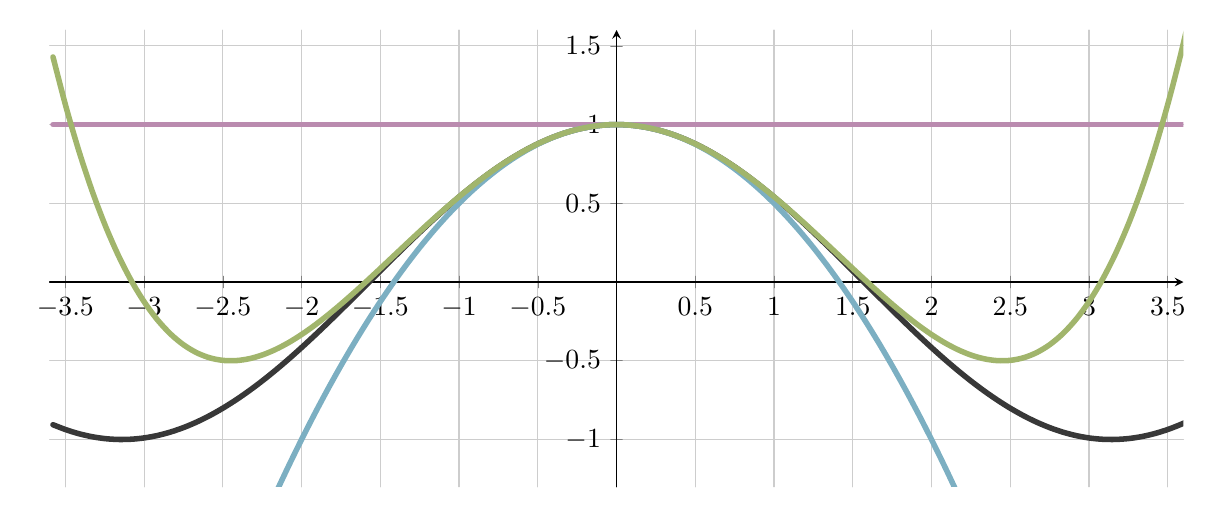
\begin{tikzpicture}[line cap=round,line join=round,>=triangle 45,x=1cm,y=1cm]
   \begin{axis}[
   x=2cm,y=2cm,
   axis lines=middle,
   ymajorgrids=true,
   xmajorgrids=true,
   xmin=-3.6, xmax=3.6,
   ymin=-1.3, ymax=1.6,
   xtick={-3.5,-3,...,3.5},
   ytick={-1.5,-1,...,1.5},]

      \draw[line width=2pt,color=black,smooth,samples=100,domain=-3.5783794469630568:4.668219928985293] plot(\x,{cos(((\x))*180/pi)});
      \draw[line width=2pt,color=purple,smooth,samples=100,domain=-3.5783794469630568:4.668219928985293] plot(\x,{1});
      \draw[line width=2pt,color=blue,smooth,samples=100,domain=-3.5783794469630568:4.668219928985293] plot(\x,{1-1/2*(\x)^(2)});
      \draw[line width=2pt,color=green,smooth,samples=100,domain=-3.5783794469630568:4.668219928985293] plot(\x,{1-1/2*(\x)^(2)+1/24*(\x)^(4)});
   \end{axis}
\end{tikzpicture}

      \end{center}
   \end{example}

   \begin{proposition}
      Let \(f: (a; b) \to \mathbb{R}\) be \(m\) times continuous differentiable and \(x_0 \in (a; b)\).
      Further is \(f'(x_0) = f''(x_0) = \ldots = f^{(m-1)}(x_0) = 0\) but \(f^{(m)}(x_0) \neq 0\), if
      \begin{enumerate}[label=\roman*, align=Center]
         \item \(m\) even and \(f^{(m)}(x_0) > 0\), then is \(x_0\) a local \textit{minimum} of \(f\).
         \item \(m\) even and \(f^{(m)}(x_0) < 0\), then is \(x_0\) a local \textit{maximum} of \(f\).
         \item \(m\) odd, then is \(x_0\) no local extrema and if \(m \geq 3\), then changes the sign of \(f''\) at \(x = x_0\).
      \end{enumerate}
   \end{proposition}

   \begin{definition}[Saddle Point]
      A point on the graph of \(f\) where \(f'(x_0) = 0\).
   \end{definition}

   \begin{definition}[Inflection Point]
      A point on a continuously differentiable plane curve at which the curve crosses its tangent, i.e. changes its curvature from concave to convex or vice versa.
   \end{definition}
   \begin{example}
      \(x^3\) has its inflection point and saddle point at \(x_0 = 0\).
      \begin{center}
         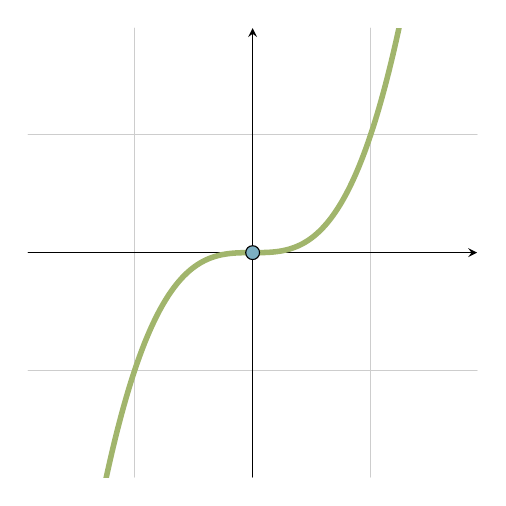
\begin{tikzpicture}[line cap=round,line join=round,>=triangle 45,x=1cm,y=1cm]
   \begin{axis}[
   ticks=none,
   x=1.5cm,y=1.5cm,
   axis lines=middle,
   ymajorgrids=true,
   xmajorgrids=true,
   xmin=-1.9, xmax=1.9,
   ymin=-1.9, ymax=1.9,
   xtick={-2,-1,...,2},
   ytick={-2,-1,...,2},]

      \draw[line width=2pt,color=green,smooth,samples=100,domain=-2:2] plot(\x,{(\x)^(3)});

      \draw [fill=blue] (0,0) circle (2.5pt);
   \end{axis}
\end{tikzpicture}

      \end{center}
   \end{example}

   \subsection{Taylor Series \& Analytic Functions}
   Suppose \(f \in C^\infty(I)\), then we can write the taylor polynomial as
   \[p_m(x) = \sum_{n=0}^m \frac{f^{(n)}(a)}{n!}(x - a)^n\]
   Since the taylor approximation implies that there exists \(p_m\) which approximates \(f\) better and better as \(m\) gets larger, it is natural to as whether the taylor series
   \[\sum_{m=0}^\infty \frac{f^{(m)}(a)}{m!}(x-a)^m\]
   converges in an intervall around \(x = a\) and if so, whether it is equal to the original function.

   \begin{example}
      Let \(f(x) = \exp(x)\).
      It holds that \(\forall n \in \mathbb{N}: f^{(n)}(x) = \exp(x)\).
      The taylor series around \(x = 0\) is
      \[\sum_{n=0}^\infty \frac{x^n}{n!}\]
      since \(f^{(n)}(0) = \exp(0) = 1\).
      It follows that the series is equal to \(\exp\) for all \(x \in \mathbb{R}\).
   \end{example}

   \begin{example}
      Let \(f(x) = \log(x)\) and we look at \(a = 1\).
      First we note that
      \[f'(x) = \frac{1}{x} \qquad f''(x) = \frac{-1}{x^2} \qquad f^{(3)}(x) = \frac{1 \cdot 2}{x^3} \qquad f^{(4)}(x) = \frac{-1 \cdot 2 \cdot 3}{x^3}\]
      This gives us the taylor polynomial
      \[\log(x) \approx \log(1) + \frac{1}{1}(x-1) + \frac{1}{2!}\frac{-1}{1^2}(x-1)^2 + \frac{1}{3!}\frac{1 \cdot 2}{1^3}(x-1)^3 + \frac{1}{4!}\frac{-1 \cdot 2 \cdot 3}{1^3}(x-1)^4\]
      which results in
      \[\log(x) \approx (x-1) - \frac{(x-1)^2}{2} + \frac{(x-1)^3}{3} - \frac{(x-1)^4}{4} + \ldots\]
      But in contrast to \(\exp\) is this approximation only accurate within some margin around \(a\), even with infinitely many terms.
      This margin is precisely the radius of convergence of the taylor series for \(\log\).

      \begin{center}
         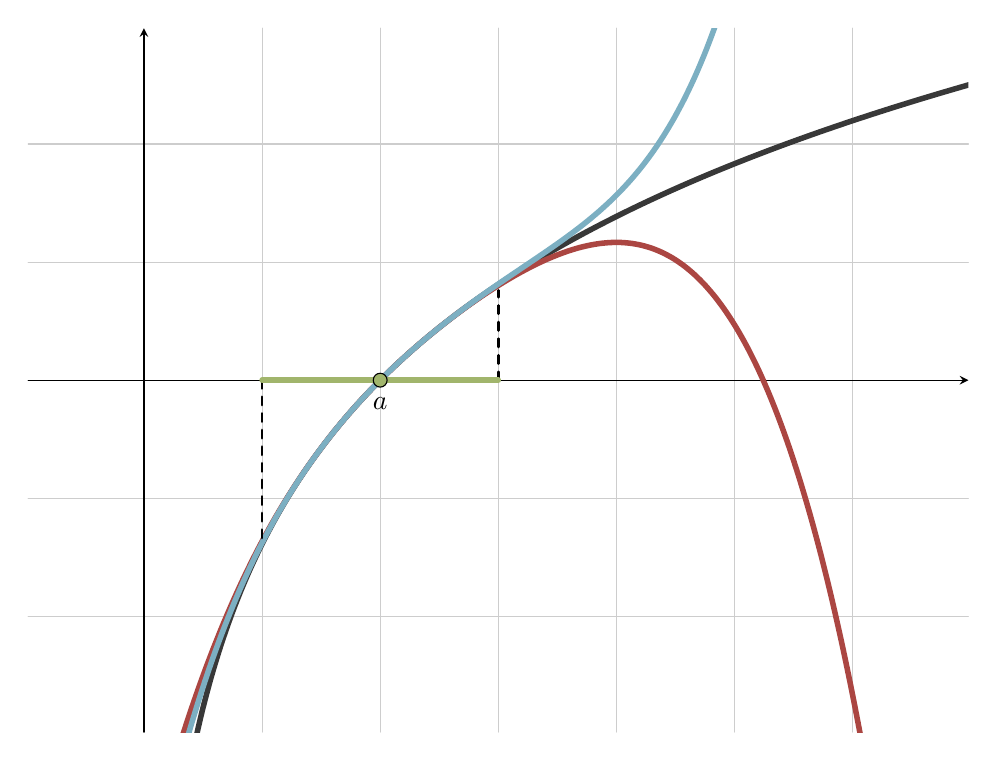
\begin{tikzpicture}[line cap=round,line join=round,>=triangle 45,x=1cm,y=1cm]
   \begin{axis}[
      ticks=none,
      x=3cm,y=3cm,
      axis lines=middle,
      ymajorgrids=true,
      xmajorgrids=true,
      xmin=-0.49, xmax=3.49,
      ymin=-1.49, ymax=1.49,]

      \draw[line width=2pt,color=black,smooth,samples=100,domain=0.000001617764269312816:3.9772961720037547] plot(\x,{ln((\x))});
      \draw[line width=2pt,color=red,smooth,samples=100,domain=-0.42494690661477774:3.9772961720037547] plot(\x,{(\x)-1-((\x)-1)^(2)/2+((\x)-1)^(3)/3-((\x)-1)^(4)/4});
      \draw[line width=2pt,color=blue,smooth,samples=100,domain=-0.42494690661477774:3.9772961720037547] plot(\x,{(\x)-1-((\x)-1)^(2)/2+((\x)-1)^(3)/3-((\x)-1)^(4)/4+((\x)-1)^(5)/5});

      \draw [line width=1pt,dashed] (1.5,0)-- (1.5,0.38);
      \draw [line width=1pt,dashed] (0.5,0)-- (0.5,-0.7);
      \draw [line width=2pt,color=green] (0.5,0)-- (1,0);
      \draw [line width=2pt,color=green] (1,0)-- (1.5, 0);

      \draw [fill=green] (1,0) circle (2.5pt);
      \draw (1, -0.1) node {\(a\)};
   \end{axis}
\end{tikzpicture}

      \end{center}
   \end{example}

   In the last example it wasn't possible to express \(f\) as a taylor series but maybe there exists a different taylor series for which it is possible.
   We define the sequence \(a_n = \frac{f^{(n)}(a)}{n!}\), suppose it holds that \(f(x) = \sum_{n=0}^\infty a_n (x-a)^n\) in a neighbourhood of \(x = a\).
   Now suppose for a moment that we can exchange the derivative and an infinite sum.
   Then is
   \[f^{(j)}(x) = \sum_{n=j}^\infty a_n n \cdot (n-1) \cdot \ldots \cdot (n-j+1)(x-a)^{n-j} \implies f^{(j)}(a) = a_j \cdot j! \implies a_j = \frac{f^{(j)}(a)}{j!}\]
   and so
   \[f(x) = \sum_{n=0}^\infty \frac{f^{(n)}(a)}{n!} (x-a)^n\]
   To state this more precisely we will show that the derivative of a power series (\ref{def:power_series}) --- in the following proposition represented as a function series --- is equal to the limit of the derivative of the partial sum is.

   Or more in general: Is the derivated limit of a function sequence equal to the limit of the derivative sequence?
   For example \(f_n(x) = \frac{\sin(nx)}{n}\) for \(x \in \mathbb{R}\) converges uniformly to 0, but \(f_n'(x) = \cos(nx)\) does not converge.
   Also \(f_n(x) = \sqrt{\frac{x^2 + 1}{n^2}}\) defined on \(\mathbb{R}\).
   \(f_n\) is overall differentiable, but \(f_n(x) \to |x|\) uniformly and \(|x|\) is not differentiable at \(x=0\).

   \begin{proposition}[Derivated Limit = Limit of Derivatives]\label{pro:deriv_limit=limit_deriv}
      Let \(I = (a;b) \subset \mathbb{R}\) and \(f_n \in C^1(I)\) a function sequence which \(f_n \to f\) and \(f_n' \to g\) uniformly on \(I\), then is
      \[f \in C^1(I) \quad\text{and}\quad f' = g\]
   \end{proposition}
   \begin{remark}
      This proposition states that
      \[\frac{d}{dx} \lim_{n \to \infty} f_n(x) = \lim_{n \to \infty} \frac{d}{dx}f_n(x)\]
   \end{remark}

   \begin{theorem}[Termwise Derivative of Power Series]\label{thm:power_series_derivative}
      Let \(\sum a_n z^n\) be a power series with \(\rho > 0\) and \(f(x) = \sum a_n x^n\) for \(|x| < \rho\), then
      \begin{enumerate}
         \item \(\sum (n+1)a_{n+1}x^n\) also has \(\rho\).
         \item \(f\) is differentiable on \((-\rho \rho)\) with
            \[f'(x) = \sum_{n=0}^\infty (n+1)a_{n+1}x^n\]
      \end{enumerate}
   \end{theorem}
   \begin{remark}
      This theorem states that power series can be differentiated termwise.
   \end{remark}

   \begin{corollary}\label{cor:termwise_derivative}
      Let \(\rho > 0\) of \(\sum_{n \geq 0} a_n x^n =: f(x)\) for \(|x| < \rho\), then is
      \[f \in C^\infty\big((-\rho; \rho)\big) \quad\text{and}\quad \forall j \in \mathbb{N}: f^{(j)}(x) = \sum_{n=0}^\infty (n+1)(n+2) \cdot \ldots \cdot (n+j)a_{n+j}x^n\]
      \[\text{Especially}~\forall j \in \mathbb{N}: f^{(j)}(0) = j!a_j \implies a_j = \frac{f^{(j)}(0)}{j!}\]
   \end{corollary}

   \begin{definition}[Analytic Function]
      \(f\) defined on \(I\) is analytic at \(x_0 \in I\) if there exists a power series with
      \[f(x) = \sum_{n \geq 0}^\infty a_n(x - x_0)^n\]
      for all \(x\) in a neighbourhood of \(x_0\).
   \end{definition}
   \begin{remark}
      From \cref{cor:termwise_derivative} follows that if \(f\) is analytic at \(x_0\) then is \(f\) infinitely differentiable at \(x_0\) and that \(\sum a_n(x - x_0)^n\) represents \(f\) in a neighbourhood of \(x_0\).
      This power series has the coefficients
      \[a_n = \frac{f^{(n)}(x_0)}{n!}\]
      This means that \(f\) is analytic at \(x_0\) iff the taylor series of \(f\) at \(x_0\) has the radius of convergence \(\rho > 0\) and if it represents \(f\) in a neighbourhood of \(x_0\).
   \end{remark}

   \begin{proposition}[Isolated Roots]\label{pro:isolated_roots}
      Let \(f\) be analytic at \(x_0\) with \(f(x_0) = 0\), then there exists an intervall \(I\) around \(x_0\) where either \(\forall x \in I: f(x) = 0\) or \(\forall x \in I \setminus \{0\}: f(x) \neq 0\).
   \end{proposition}

   \begin{theorem}[Identity Principle]\label{thm:identiy_principle}
      Let \(f, g\) be analytic at \(x_0\), \(\exists (x_n)_{n \in \mathbb{N}}\) with \(x_n \neq x_0\), \(x_n \to x_0\) and \(f(x_n) = g(x_n)\) for all \(n \in \mathbb{N}\), then
      \[\exists I: (\forall x \in I: f(x) = g(x))\]
      an open intervall around \(x_0\).
   \end{theorem}

   \begin{proposition}
      Let \(f\) be analytic at \(x_0\) and \(\forall x: |x-x_0| < \rho: (f(x) = \sum a_n(x-x_0)^n)\), then is \(f\) analytic at \(x_1\), \(\forall x_1: |x_1 - x_0| < \rho\).
      Further holds for \(|x - x_1| < \widetilde{\rho} = \rho - |x_1 - x_0|\)
      \[f(x) = \sum_{j=0}^\infty b_j (x - x_0)^j \quad\text{where}\quad b_j = \sum_{n \geq j} \binom{n}{j}a_n(x_1 - x_0)^{n-j} = \sum_{m=0}^\infty \binom{j+m}{j} a_{m+j}(x_1 - x_0)^m\]
   \end{proposition}

   Some more facts about functions which are analytic at \(x_0\):
   \begin{enumerate}
      \item \(f, g~\text{analytic} \implies f \cdot g~\text{analytic}\)
      \item \(f~\text{analytic with}~f(x_0) \neq 0 \implies \frac{1}{f}~\text{analytic}\)
      \item \(f~\text{analytic and}~g~\text{analytic at}~f(x_0) \implies g \circ f~\text{analytic at}~x_0\)
      \item \(f~\text{analytic and invertible and}~f'(x_0) \neq 0 \implies f^{-1}~\text{analytic at}~f(x_0)\)
   \end{enumerate}

   \section{Riemann Integral}
   \subsection{Definition \& Basic Properties}
   The basic idea is that we want to calculate (and define) for \(f: [a; b] \to [0; \infty)\) the surface area of \(\{(x, y) \mid x \in [a; b], y \in [0; f(x)]\}\).
   Intuitively we chose \(x_0, \ldots, x_n \in \mathbb{R}: a = x_0 < \ldots < x_n = b\) which partitions \([a; b]\) in \(n\) intervalls \([x_0; x_1], [x_1; x_2], \ldots, [x_{n-1}; x_n]\).
   Then we chose representatives \(\xi_j \in [x_{j-1}; x_j]\) and calculate the area of each partition with \(f(\xi_j) \cdot (x_j - x_{j-1})\).

   \begin{center}
      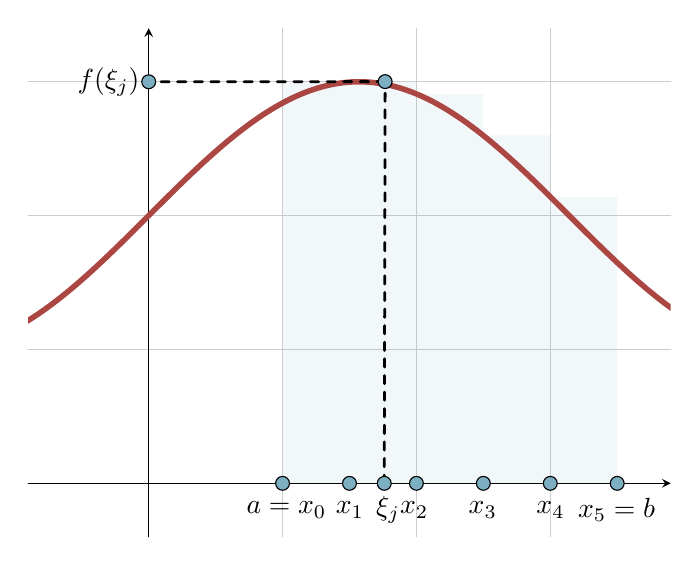
\begin{tikzpicture}[line cap=round,line join=round,>=triangle 45,x=1cm,y=1cm]
   \begin{axis}[
   ticks=none,
   x=1.7cm,y=1.7cm,
   axis lines=middle,
   ymajorgrids=true,
   xmajorgrids=true,
   xmin=-0.9, xmax=3.9,
   ymin=-0.4, ymax=3.4,]

   \fill[line width=2pt,color=blue,fill=blue,fill opacity=0.1] (0.9999995508667879,3.0006701738657333) -- (2,3) -- (2,0) -- (1,0) -- cycle;
   \fill[line width=2pt,color=blue,fill=blue,fill opacity=0.1] (2.5,0) -- (2,0) -- (2,2.909297426825682) -- (2.5003489959712746,2.9096194363833323) -- cycle;
   \fill[line width=2pt,color=blue,fill=blue,fill opacity=0.1] (3,0) -- (2.5,0) -- (2.500311645280321,2.598222442418714) -- (3,2.6) -- cycle;
   \fill[line width=2pt,color=blue,fill=blue,fill opacity=0.1] (3.5,0) -- (3,0) -- (3,2.1411200080598674) -- (3.5003490895130804,2.140237672611229) -- cycle;

   \draw[line width=2pt,color=red,smooth,samples=100,domain=-1:4] plot(\x,{sin(((\x))*180/pi)+2});

   \draw [line width=1pt,dashed] (1.7598222492782805,0)-- (1.766437939924849,3.001183821074471);
   \draw [line width=1pt,dashed] (1.766437939924849,3.001183821074471)-- (0,3);

   \draw [fill=blue] (1,0) circle (2.5pt);
   \draw (1.0295099272672354,-0.2) node {$a = x_0$};
   \draw [fill=blue] (3.5,0) circle (2.5pt);
   \draw (3.495331993290693,-0.2) node {$x_5 = b$};
   \draw [fill=blue] (1.5,0) circle (2.5pt);
   \draw (1.5032073241612158,-0.2) node {$x_1$};
   \draw [fill=blue] (2,0) circle (2.5pt);
   \draw (1.9833937264920998,-0.2) node {$x_2$};
   \draw [fill=blue] (2.5,0) circle (2.5pt);
   \draw (2.4960251560075024,-0.2) node {$x_3$};
   \draw [fill=blue] (3,0) circle (2.5pt);
   \draw (3.0021675800860015,-0.2) node {$x_4$};
   \draw [fill=blue] (1.7598222492782805,0) circle (2.5pt);
   \draw (1.7887235633849845,-0.2) node {$\xi_j$};
   \draw [fill=blue] (0,3) circle (2.5pt);
   \draw (-0.3,3) node {$f(\xi_j)$};
   \draw [fill=blue] (1.766437939924849,3.001183821074471) circle (2.5pt);
   \end{axis}
\end{tikzpicture}

   \end{center}

   The whole area is then the \textit{riemann sum}
   \[\sum_{j=1}^n f(\xi_j) \cdot (x_j - x_{j-1})\]
   Now we hope that this sum converges since the partitioning is infinitesimal accurate.
   The integral is then defined as the limit of the sum.

   \begin{definition}[Partition of Intervall]
      Given an intervall \(I = [a; b]\)
      \[(x_n)_{n \in \mathbb{N}}: a = x_0 < x_1 < \ldots x_k = b\]
   \end{definition}
   \begin{remark}
      For a given partition \(T\) of \(I\) we say \(I_j = [x_{j-1}; x_j]\) is a \textit{subintervall} of \(T\).
      It holds that
      \[I = \bigcup_{j=1}^n I_j \qquad\text{and}\qquad I_j \cap I_{j+1} = \{x_j\}\]
      for an \(n\)-tuple of representatives \(\xi = (\xi_1, \ldots, \xi_n)\) where \(\forall j \in [1; n]: \xi_j \in I_j\)
   \end{remark}

   \begin{definition}[Riemann Sum]
      Given a partition \(T\) and an \(n\)-tuple of representatives \(\xi\).
      \[S(T, \xi) := \sum_{j=1}^n f(\xi_j) \cdot (x_j - x_{j-1}) = \sum_{j=1}^n f(\xi_j) \cdot |I_j|\]
   \end{definition}
   \begin{remark}
      \(f(\xi_j)\) is the height of the rectangles and \(|I_j|\) are their widths.
      \(|I_j|\) is defined through \(T\).
   \end{remark}

   \begin{definition}[Upper/Lower Rieman Sum]
      Given a partition \(T\) and an \(n\)-tuple of representatives \(\xi\).
      \[\overline{S}(T) := \sup_{\xi} S(T, \xi) = \sum_{j=1}^n \sup\{f(x) \mid x \in I_j\} \cdot |I_j|\]
      \[\underline{S}(T) := \inf_{\xi} S(T, \xi) = \sum_{j=1}^n \inf\{f(x) \mid x \in I_j\} \cdot |I_j|\]
   \end{definition}
   \begin{remark}
      For all partitions \(T\) holds \(\underline{S}(T) \leq \overline{S}(T)\) and intuitivly is the lower sum smaller than the surface area and the upper sum bigger.
   \end{remark}

   \begin{center}
      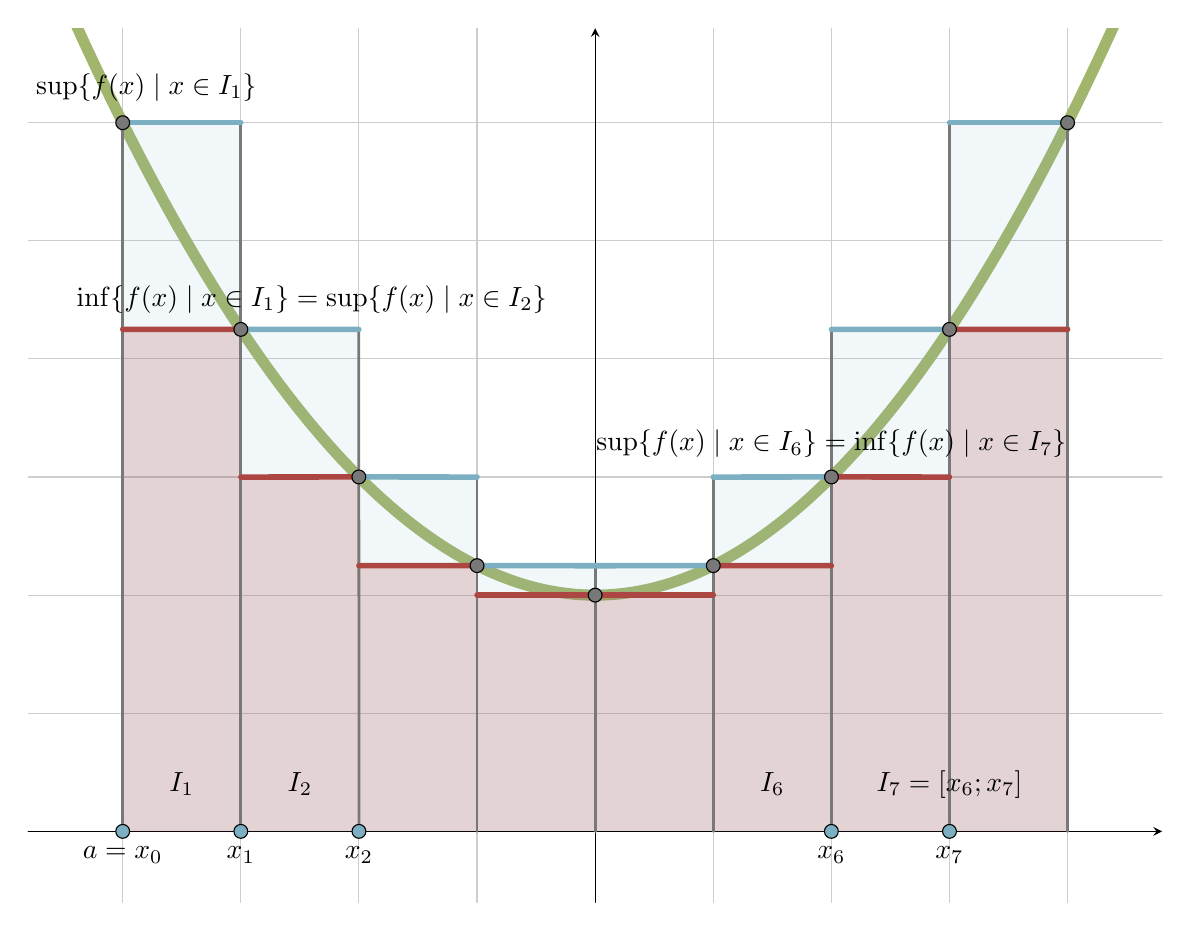
\begin{tikzpicture}[line cap=round,line join=round,>=triangle 45,x=1cm,y=1cm]
   \begin{axis}[
      ticks=none,
      x=3cm,y=3cm,
      axis lines=middle,
      ymajorgrids=true,
      xmajorgrids=true,
      xmin=-2.4, xmax=2.4,
      ymin=-0.3, ymax=3.4,]

      \draw[line width=4pt,color=green,smooth,samples=100,domain=-3.035521966081091:3.181639604487395] plot(\x,{1/2*(\x)^(2)+1});

      \fill[line width=2pt,color=blue,fill=blue,fill opacity=0.10000000149011612] (-2,0) -- (-2,3) -- (-1.5,3) -- (-1.5,0) -- cycle;
      \fill[line width=2pt,color=blue,fill=blue,fill opacity=0.10000000149011612] (-1.5,0) -- (-1.5,2.125) -- (-1.000492193985458,2.124719018243788) -- (-1,0) -- cycle;
      \fill[line width=2pt,color=blue,fill=blue,fill opacity=0.10000000149011612] (-1,0) -- (-1.0003475575204508,1.5003476179185657) -- (-0.5,1.5) -- (-0.5,0) -- cycle;
      \fill[line width=2pt,color=blue,fill=blue,fill opacity=0.10000000149011612] (-0.5,0) -- (-0.5,1.125) -- (0,1.124425296538493) -- (0,0) -- cycle;
      \fill[line width=2pt,color=blue,fill=blue,fill opacity=0.10000000149011612] (2,0) -- (2,3) -- (1.5,3) -- (1.5,0) -- cycle;
      \fill[line width=2pt,color=blue,fill=blue,fill opacity=0.10000000149011612] (0,1.124425296538493) -- (0.5,1.125) -- (0.5,0) -- (0,0) -- cycle;

      \fill[line width=2pt,color=red,fill=red,fill opacity=0.2] (-2,0) -- (-1.5,0) -- (-1.5,2.125) -- (-2,2.125464867600505) -- cycle;
      \fill[line width=2pt,color=red,fill=red,fill opacity=0.2] (-1.5,0) -- (-1,0) -- (-1.0003475575204508,1.5003476179185657) -- (-1.5,1.5) -- cycle;
      \fill[line width=2pt,color=red,fill=red,fill opacity=0.2] (-1,0) -- (-0.5,0) -- (-0.5,1.125) -- (-1.000260570435978,1.1248389400761278) -- cycle;
      \fill[line width=2pt,color=red,fill=red,fill opacity=0.2] (-0.5,0) -- (0,0) -- (0,1) -- (-0.5,1) -- cycle;
      \fill[line width=2pt,color=blue,fill=blue,fill opacity=0.10000000149011612] (1,0) -- (0.5,0) -- (0.5,1.5) -- (1.000347557520451,1.5003476179185655) -- cycle;
      \fill[line width=2pt,color=blue,fill=blue,fill opacity=0.10000000149011612] (1.5,0) -- (1.5,2.125) -- (1.0004921939854583,2.124719018243788) -- (1,0) -- cycle;
      \fill[line width=2pt,color=red,fill=red,fill opacity=0.2] (0,1) -- (0.5,1) -- (0.5,0) -- (0,0) -- cycle;
      \fill[line width=2pt,color=red,fill=red,fill opacity=0.2] (0.5,1.125) -- (1.0002605704359782,1.1248389400761276) -- (1,0) -- (0.5,0) -- cycle;
      \fill[line width=2pt,color=red,fill=red,fill opacity=0.2] (1.000347557520451,1.5003476179185655) -- (1.5,1.5) -- (1.5,0) -- (1,0) -- cycle;
      \fill[line width=2pt,color=red,fill=red,fill opacity=0.2] (1.5,2.125) -- (2,2.1254648676005043) -- (2,0) -- (1.5,0) -- cycle;

      \draw [line width=1pt,color=grey] (2,0)-- (2,3);
      \draw [line width=1pt,color=grey] (0,0)-- (0,1.124425296538493);
      \draw [line width=1pt,color=grey] (0.5,0)-- (0.5,1.5);
      \draw [line width=1pt,color=grey] (1.0004921939854583,2.124719018243788)-- (1,0);
      \draw [line width=1pt,color=grey] (1.5,3)-- (1.5,0);
      \draw [line width=1pt,color=grey] (-1.000492193985458,2.124719018243788)-- (-1,0);
      \draw [line width=1pt,color=grey] (-2,0)-- (-2,3);
      \draw [line width=1pt,color=grey] (-1.5,3)-- (-1.5,0);
      \draw [line width=1pt,color=grey] (-0.5,1.5)-- (-0.5,0);
      \draw [line width=2pt,color=blue] (-2,3)-- (-1.5,3);
      \draw [line width=2pt,color=blue] (-1.5,2.125)-- (-1.000492193985458,2.124719018243788);
      \draw [line width=2pt,color=blue] (-1.0003475575204508,1.5003476179185657)-- (-0.5,1.5);
      \draw [line width=2pt,color=blue] (-0.5,1.125)-- (0,1.124425296538493);
      \draw [line width=2pt,color=blue] (2,3)-- (1.5,3);
      \draw [line width=2pt,color=blue] (0,1.124425296538493)-- (0.5,1.125);
      \draw [line width=2pt,color=red] (-1.5,2.125)-- (-2,2.125464867600505);
      \draw [line width=2pt,color=red] (-1.0003475575204508,1.5003476179185657)-- (-1.5,1.5);
      \draw [line width=2pt,color=red] (-0.5,1.125)-- (-1.000260570435978,1.1248389400761278);
      \draw [line width=2pt,color=red] (0,1)-- (-0.5,1);
      \draw [line width=2pt,color=blue] (0.5,1.5)-- (1.000347557520451,1.5003476179185655);
      \draw [line width=2pt,color=blue] (1.5,2.125)-- (1.0004921939854583,2.124719018243788);
      \draw [line width=2pt,color=red] (0,1)-- (0.5,1);
      \draw [line width=2pt,color=red] (0.5,1.125)-- (1.0002605704359782,1.1248389400761276);
      \draw [line width=2pt,color=red] (1.000347557520451,1.5003476179185655)-- (1.5,1.5);
      \draw [line width=2pt,color=red] (1.5,2.125)-- (2,2.1254648676005043);

      \draw (-1.9, 3.15) node {$\sup\{f(x) \mid x \in I_1\}$};
      \draw (-1.2, 2.25) node {$\inf\{f(x) \mid x \in I_1\} = \sup\{f(x) \mid x \in I_2\}$};
      \draw (1, 1.64) node {$\sup\{f(x) \mid x \in I_6\} = \inf\{f(x) \mid x \in I_7\}$};

      \draw [fill=blue] (-2,0) circle (2.5pt);
      \draw (-2,-0.1) node {$a = x_0$};
      \draw [fill=grey] (-2,3) circle (2.5pt);
      \draw [fill=blue] (-1.5,0) circle (2.5pt);
      \draw (-1.5, -0.1) node {$x_1$};
      \draw [fill=grey] (-1.5,2.125) circle (2.5pt);
      \draw [fill=blue] (-1,0) circle (2.5pt);
      \draw (-1, -0.1) node {$x_2$};
      \draw [fill=grey] (-1.0003475575204508,1.5003476179185657) circle (2.5pt);
      \draw [fill=grey] (-0.5,1.125) circle (2.5pt);
      \draw [fill=grey] (2,3) circle (2.5pt);
      \draw [fill=blue] (1.5,0) circle (2.5pt);
      \draw (1.5, -0.1) node {$x_7$};
      \draw [fill=grey] (1.5,2.125) circle (2.5pt);
      \draw [fill=blue] (1,0) circle (2.5pt);
      \draw (1, -0.1) node {$x_6$};
      \draw [fill=grey] (1.000347557520451,1.5003476179185655) circle (2.5pt);
      \draw [fill=grey] (0.5,1.125) circle (2.5pt);
      \draw [fill=grey] (0,1) circle (2.5pt);
      \draw (-1.75, 0.2) node {$I_1$};
      \draw (-1.25, 0.2) node {$I_2$};
      \draw (0.75, 0.2) node {$I_6$};
      \draw (1.5, 0.2) node {$I_7 = [x_6; x_7]$};
   \end{axis}
\end{tikzpicture}

   \end{center}

   \begin{remark}
      We call \(T' \supset T\) a \textit{refinement} of \(T\).
      This means that we keep already existing \(x_j \in T\) and add even more.
      This results in that \(\overline{S}\) gets smaller while \(\underline{S}\) gets bigger.
   \end{remark}
   \begin{lemma}\label{lem:refinement_of_partition}
      Let \(T\) be a partition and \(T' \supset T\) be its refinement, then holds
      \begin{enumerate}[label=\roman*, align=Center]
         \item \(\overline{S}(T') \leq \overline{S}(T)\) and \(\underline{S}(T') \geq \underline{S}(T)\)
         \item \(\sup_T \underline{S}(T) \leq \inf_T \overline{S}(T)\)
      \end{enumerate}
   \end{lemma}

   \begin{definition}[Riemann Integral]
      A bounded \(f: [a; b] \to \mathbb{R}\) is Riemann integrable if
      \[\sup_{T}\underline{S}(T) = \inf_{T}\overline{S}(T)~\text{then we define}\quad \int_a^b f(x) dx := \sup_{T}\underline{S}(T) = \inf_{T}\overline{S}(T)\]
   \end{definition}

   \begin{proposition}\label{pro:integrable}
      Let \(f: [a; b] \to \mathbb{R}\) be bounded.
      \begin{enumerate}[label=\roman*, align=Center]
         \item \(f~\text{integrable} \iff \inf_{T}(\overline{S}(T) - \underline{S}(T)) = 0 \iff \inf_{T}(\overline{S}(T) - \underline{S}(T)) \leq 0\)
            \item Let \((T_n)_{n \in \mathbb{N}}: \overline{S}(T_n) - \underline{S}(T) \xrightarrow{n \to \infty} 0\), then is \(f\) integrable and
               \[\overline{S}(T_n) \to \int_a^b f(x) dx \qquad \underline{S}(T_n) \to \int_a^b f(x) dx\]
               Futhermore if \(\xi_n\) is an arbitrary family of representatives of \(T_n\), then
               \[S(T_n, \xi_n) \to \int_a^b f(x) dx\]
      \end{enumerate}
   \end{proposition}

   \begin{definition}[Oscillation of Function]\label{def:oscillation}
      Given a set \(J\) and \(f: J \to \mathbb{R}\)
      \[\sigma(f, J) := \sup\{f(x) \mid x \in J\} - \inf\{f(x) \mid x \in J\} = \sup\{|f(x) - f(y)| \mid x, y \in J\]
   \end{definition}
   \begin{remark}
      The oscillation of a function is a number that quantifies how much a sequence or function varies between its extreme values as it approaches infinity or a point.
      For an arbitrary partition \(T\) holds
      \[\overline{S}(T) - \underline{S}(T) = \sum_{j=1}^n \sigma(f, I_j) \cdot |I_j|\]
   \end{remark}

   \begin{remark}[Longest Interval]
      Given a partition \(T\) of \([a; b]\) we set
      \[\|T\| := \max_{j = 1, \ldots, n}|x_j - x_{j-1}|\]
      which is the length of the biggest intervall in \(T\).
   \end{remark}

   \begin{proposition}\label{pro:biggest_intervall_converges}
      Let \(f\) be integrable on \([a;b]\), \((T_n)_{n \in \mathbb{N}}: \|T_n\| \to 0\) and \(\forall n \in \mathbb{N}: \xi_n\) be a family of representatives for \(T_n\), then is
      \[\int_a^b f(x) dx = \lim_{n \to \infty} \overline{S}(T_n) = \lim_{n \to \infty} \underline{S}(T_n) = \lim_{n \to \infty} S(T_n \xi_n)\]
   \end{proposition}
   \begin{remark}
      This proposition states, that we don't have to regard infinitely many partitions.
      We only need one where \(\|T_n\| \to 0\) and \(\lim \overline{S}(T_n) = \lim \underline{S}(T_n)\), then gives us the limit the value of the integral.
   \end{remark}

   \begin{proposition}[Continuity \(\implies\) Integrability]\label{pro:cont_impl_integr}
      Is \(f\) continuous on \([a;b]\), then is \(f\) integrable on \([a;b]\).
   \end{proposition}
   \begin{example}
      Let \(f(x) = \frac{1}{x}\).
      \(f\) is continuous on \([1; a]\) for \(a > 1\) hence \(f\) is integrable on \([1; a]\).
      We choose a partition
      \[T_n = \{(\sqrt[n]{a})^j \mid j \in [0; n]\} \implies I_j = \big[(\sqrt[n]{a})^{j-1}; (\sqrt[n]{a})^j\big]~\text{for}~j = 1, \ldots, n\]
      \[\frac{1}{x}~\text{decreasing} \implies \sup\{f(x) \mid x \in I_j\} = \frac{1}{(\sqrt[n]{a})^{j-1}} \quad\text{and}\quad \inf\{f(x) \mid x \in I_j\} = \frac{1}{(\sqrt[n]{a})^j}\]
      So we get the followsing riemann sums
      \[\underline{S}(T_n) = \sum_{j=1}^n \frac{1}{(\sqrt[n]{a})^j} \cdot \big((\sqrt[n]{a})^j - (\sqrt[n]{a})^{j-1}\big) = \sum_{j=1}^n \big(1 - \sqrt[n]{a}^{-1}\big) = n \left(1 - \frac{1}{\sqrt[n]{a}}\right)\]
      \[\overline{S}(T_n) = \sum_{j=1}^n \frac{1}{(\sqrt[n]{a})^{j-1}} \cdot \big((\sqrt[n]{a})^j - (\sqrt[n]{a})^{j-1}\big) = \sum_{j=1}^n \frac{1}{(\sqrt[n]{a})^{-1}} \cdot \big(1 - \sqrt[n]{a}^{-1}\big) = \sqrt[n]{a} \cdot \underline{S}(T_n)\]
      Now let \(g(t) := a^t\)
      \[\underline{S}(T_n) = n \left(1 - \frac{1}{\sqrt[n]{a}}\right) = \frac{1 - a^{\frac{-1}{n}}}{\frac{1}{n}} = \frac{g(0) - g\left(-\frac{1}{n}\right)}{\frac{1}{n}}\]
      \[\lim_{n \to \infty} \underline{S}(T_n) = \lim_{n \to \infty}\frac{g(0) - g\left(-\frac{1}{n}\right)}{\frac{1}{n}} = g'(0) = \log(a)\]
      So
      \[\overline{S}(T_n) = \sqrt[n]{a}\underline{S}(T_n) \xrightarrow{n \to \infty} \log(a) \implies \int_1^a \frac{1}{x}dx = \log(a)\]
   \end{example}

   \begin{proposition}[Split Integrals]\label{pro:split_integrals}
      Let \(a < b < c\) and \(f: [a; c] \to \mathbb{R}\) be bounded, then is
      \[f~\text{integrable on}~[a;c] \iff f~\text{integrable on}~[a;b]~\text{and}~[b;c]\]
      \[\int_a^c f(x) dx = \int_a^b f(x) dx + \int_b^c f(x) dx\]
   \end{proposition}

   \begin{proposition}[Discontinuous still Integrable]\label{pro:discont_integrable}
      Let \(f: [a;b] \to \mathbb{R}\) be bounded, with finite many points of discontinuity, then is \(f\) still integrable on \([a;b]\).
   \end{proposition}

   \begin{proposition}[Integral Calculation Rules]\label{pro:integra_calc_rules}
      Let \(f, b\) be integrable on \([a;b]\), then holds
      \begin{enumerate}[label=\roman*, align=Center]
         \item Linearity: \(\forall \alpha, \beta: \alpha f + \beta g\) integrable
            \[\int_a^b(\alpha f + \beta g)dx = \alpha \int_a^b f(x) dx + \beta \int_a^b g(x) dx\]
         \item Monotony: If \(\forall x \in [a; b]: f(x) \geq g(x)\) then is
            \[\int_a^b f(x) dx \geq \int_a^b g(x)dx\]
         \item Triangle Intequality: \(|f|\) is integrable
            \[\left|\int_a^b f(x) dx\right| \leq \int_a^b |f(x)| dx\]
            \[\min(f, g)~\text{and}~\max(f, g)~\text{are integrable}\]
      \end{enumerate}
   \end{proposition}

   \begin{theorem}\label{thm:conesq_calc_rules}
      \begin{enumerate}[label=\roman*, align=Center]
         \item Constant functions are integrable
            \[\int_a^b c~dx = c (b - a)\]
         \item Let \(f\) be integrable on \([a; b]\) and \(m := \inf\{f(x) \mid x \in [a;b]\}\), \(M := \sup\{f(x) \mid x \in [a;b]\}\), then is
            \[m(b-a) \leq \int_a^b f(x) dx \leq M (b-a)\]
         \item Mean Value: Is \(f\) continuous on \([a;b]\), then
            \[\exists \xi \in (a; b): \int_a^b f(x)dx = f(\xi)(b-a)\]
      \end{enumerate}
   \end{theorem}

   \begin{center}
      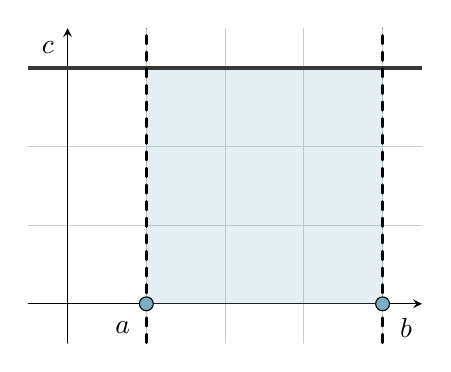
\begin{tikzpicture}[line cap=round,line join=round,>=triangle 45,x=1cm,y=1cm]
   \begin{axis}[
      ticks=none,
      x=1cm,y=1cm,
      axis lines=middle,
      ymajorgrids=true,
      xmajorgrids=true,
      xmin=-0.5, xmax=4.5,
      ymin=-0.5, ymax=3.5,]

      \fill[line width=2pt,color=blue,fill=blue,fill opacity=0.2] (1,3) -- (4,3) -- (4,0) -- (1,0) -- cycle;
      \draw [line width=1.5pt,color=black,domain=-2.872436747088137:9.868843916771926] plot(\x,{(--15-0*\x)/5});
      \draw [line width=1pt,dashed] (1,-1.9696995359130918) -- (1,5.878342583520441);
      \draw [line width=1pt,dashed] (4,-1.9696995359130918) -- (4,5.878342583520441);

      \draw (-0.25,3.25) node {\(c\)};
      \draw [fill=blue] (1,0) circle (2.5pt);
      \draw (0.7,-0.3) node {\(a\)};
      \draw [fill=blue] (4,0) circle (2.5pt);
      \draw (4.3, -0.3) node {\(b\)};
   \end{axis}
\end{tikzpicture}

      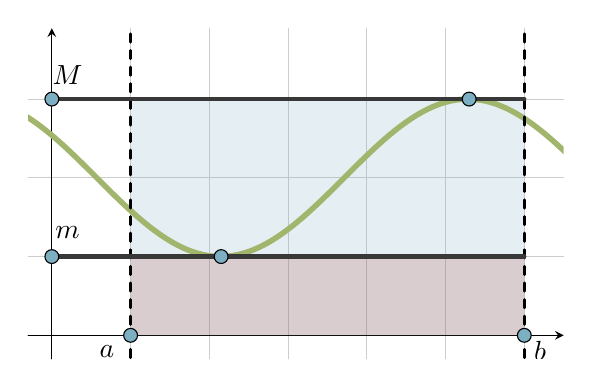
\begin{tikzpicture}[line cap=round,line join=round,>=triangle 45,x=1cm,y=1cm]
   \begin{axis}[
   ticks=none,
   x=1cm,y=1cm,
   axis lines=middle,
   ymajorgrids=true,
   xmajorgrids=true,
   xmin=-0.3, xmax=6.5,
   ymin=-0.3, ymax=3.9,]

      \fill[line width=2pt,color=blue,fill=blue,fill opacity=0.2] (1,2.999973327619512) -- (6,3) -- (6,0) -- (1,0) -- cycle;
      \fill[line width=2pt,color=red,fill=red,fill opacity=0.2] (1,1.000016437920306) -- (6,1) -- (6,0) -- (1,0) -- cycle;

      \draw[line width=2pt,color=green,smooth,samples=100,domain=-2.4605421282524333:9.895360332465595] plot(\x,{cos(((\x)+1)*180/pi)+2});

      \draw [line width=1pt,dashed] (1,-2.181083167331856) -- (1,5.429583726646621);
      \draw [line width=1pt,dashed] (6,-2.181083167331856) -- (6,5.429583726646621);
      \draw [line width=1.5pt,color=black] (0,3)-- (6,3);
      \draw [line width=1.5pt,color=black] (0,1)-- (6,1);

      \draw [fill=blue] (1,0) circle (2.5pt);
      \draw (0.7,-0.2) node {\(a\)};
      \draw [fill=blue] (6,0) circle (2.5pt);
      \draw (6.2,-0.2) node {\(b\)};
      \draw [fill=blue] (0,3) circle (2.5pt);
      \draw (0.2, 3.3) node {\(M\)};
      \draw [fill=blue] (5.3,2.999858636383415) circle (2.5pt);
      \draw [fill=blue] (0,1) circle (2.5pt);
      \draw (0.2, 1.3) node {\(m\)};
      \draw [fill=blue] (2.15,1.000035341528658) circle (2.5pt);
   \end{axis}
\end{tikzpicture}

      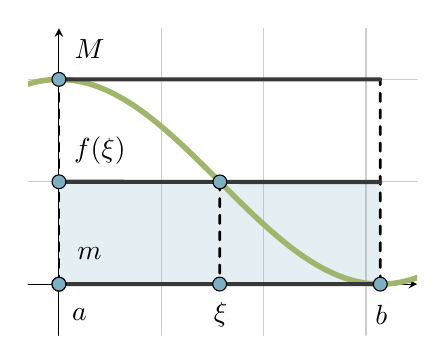
\begin{tikzpicture}[line cap=round,line join=round,>=triangle 45,x=1cm,y=1cm]
   \begin{axis}[
      ticks=none,
      x=1.3cm,y=1.3cm,
      axis lines=middle,
      ymajorgrids=true,
      xmajorgrids=true,
      xmin=-0.3, xmax=3.5,
      ymin=-0.5, ymax=2.5,]
      \fill[line width=2pt,color=blue,fill=blue,fill opacity=0.2] (0,1) -- (3.1389302441322537,0.9973204850567711) -- (3.1396040361160336,0.0000019772990768052168) -- (0,0) -- cycle;

      \draw[line width=2pt,color=green,smooth,samples=100,domain=-1.3986803002239279:4.930997461233805] plot(\x,{cos(((\x))*180/pi)+1});

      \draw [line width=1pt,dashed] (0,0)-- (0,2);
      \draw [line width=1pt,dashed] (3.1396040361160336,0.0000019772990768052168)-- (3.1382529320756967,1.9998492562393877);
      \draw [line width=1pt,dashed] (1.5721383666698445,0.9986579605279036)-- (1.569847088272582,0.0005231041652430186);
      \draw [line width=1.5pt,color=black] (0,0)-- (3.1396040361160336,0.0000019772990768052168);
      \draw [line width=1.5pt,color=black] (0,2)-- (3.1382529320756967,1.9998492562393877);
      \draw [line width=1.5pt,color=black] (0,1)-- (3.1389302441322537,0.9973204850567711);

      \draw [fill=blue] (0,0) circle (2.5pt);
      \draw (0.2, -0.3) node {\(a\)};
      \draw [fill=blue] (0,2) circle (2.5pt);
      \draw (0.3, 2.3) node {\(M\)};
      \draw [fill=blue] (3.1396040361160336,0.0000019772990768052168) circle (2.5pt);
      \draw (3.15,-0.3) node {\(b\)};
      \draw [fill=blue] (0,0) circle (2.5pt);
      \draw (0.3,0.3) node {\(m\)};
      \draw [fill=blue] (0,1) circle (2.5pt);
      \draw (0.4,1.3) node {\(f(\xi)\)};
      \draw [fill=blue] (1.5721383666698445,0.9986579605279036) circle (2.5pt);
      \draw [fill=blue] (1.569847088272582,0.0005231041652430186) circle (2.5pt);
      \draw (1.58,-0.3) node {\(\xi\)};
   \end{axis}
\end{tikzpicture}

   \end{center}

   \subsection{Fundamental Theorem of Integral Calculus}
   The followsing theorem allows us to calculate the integral of continuous functions.
   \begin{theorem}\label{thm:fund_thm_integ}
      Let \(f\) be continuous on \([a;b]\), then is for some \(x \in (a; b]\)
      \[F(x) = \int_a^x f(t)dt\]
      \begin{enumerate}[label=\roman*, align=Center]
         \item \(F\) differentiable on \((a;b)\) with \(F'(x) = f(x)\).
         \item Let \(G\) be continuous on \([a;b]\) and differentiable on \((a;b)\) with \(G'(x) = f(x)\), then is
            \[\forall x \in (a; b]: F(x) = G(x) - G(a)\]
      \end{enumerate}
   \end{theorem}

   \begin{definition}[Antiderivative]
      Given \(f\) continuous on \([a;b]\).
      The \textit{antiderivative} of \(f\) is a function \(G\), continuous on \([a;b]\) and differentiable on \((a;b)\) with
      \[\forall x \in (a;b): G'(x) = f(x)\]
      It holds that
      \[\int_a^b f(x) dx = G(b) - G(a)\]
   \end{definition}
   \begin{remark}
      The existence of an antiderivative does not imply that \(f\) is integriable.
   \end{remark}
   \begin{remark}
      If \(G\) is an antiderivative of \(f\) then is also \(G + c\) for some \(c \in \mathbb{R}\) an antiderivative of \(f\).
      We define the family of all antiderivatives of \(f\) (created by the constant \(c\)) to be the \textit{indefinite integral}.
   \end{remark}

   \begin{definition}[Indefinite Integral]
      Given a continuous function \(f\) and its antiderivative \(G\) where \(G'(x) = f(x)\).
      \[\int f(x) dx = G(x) + c\]
   \end{definition}
   \begin{remark}
      To summarize:
      The definite integral \(\int_a^b f(x) dx\) is the limit of the Riemann sums.
      The indefinite integral \(\in f(x) dx\) is a family of antiderivatives.
      According to the fundamental theorem is the computation of indefinite integrals very helpful to calculate a definite integral.
   \end{remark}

   \begin{remark}[Notation]
      For \(b < a\) we define
      \[\int_a^b f(x) dx := -\int_b^a f(x)dx\]
      and for \(b = a\) we write
      \[\int_a^a f(x) dx := 0\]
      This way we can write
      \[\int_a^b f(x) dx = G(b) - G(a)\]
      if \(f\) is continuous and \(G\) is an antiderivative of \(f\) independent of the order of \(a\) and \(b\).
   \end{remark}

   \begin{remark}[Indefinite Integrals]
      The following is a list of indefinite integrals whose antiderivatives can be represented with elementary functions.

      \(\forall \alpha: \alpha < 0 \land \alpha \neq -1\) and \(\forall x \neq 0\)
      \[\frac{d}{dx} x^\alpha = \alpha \cdot x^{\alpha - 1} \implies \int x^\alpha dx = \frac{1}{\alpha + 1} x^{\alpha + 1} + c\]
      \[\forall x \neq 0: \frac{d}{dx} \log(|x|) = \frac{1}{x} \implies \int \frac{1}{x} dx = \log(|x|) + c\]
      \[\frac{d}{dx} e^{\lambda \cdot x} = \lambda \cdot e^{\lambda \cdot x} \implies \int e^{\lambda \cdot x} dx = \frac{1}{\lambda} \cdot e^{\lambda \cdot x} + c\]
      \[\frac{d}{dx} \sin(x) = \cos(x) \implies \int \cos(x) dx = \sin(x) + c\]
      \[\frac{d}{dx} \cos(x) = -\sin(x) \implies \int \sin(x) dx = -\cos(x)dx\]
      \[\forall x \neq \frac{\pi}{2} + k\pi: \frac{d}{dx} \tan(x) = \frac{1}{\cos(x)^2} \implies \int \frac{1}{\cos(x)^2} = \tan(x)\]
      \[\forall x \in (-1;1): \frac{d}{dx} \arcsin(x) = \frac{1}{\sqrt{1 - x^2}} \implies \int \frac{1}{\sqrt{1 - x^2}}dx = \arcsin(x) + c\]
      \[\frac{d}{dx} \arccos(x) = \frac{-1}{\sqrt{1 - x^2}} \implies \int \frac{-1}{\sqrt{1 - x^2}} = \arccos(x) + c\]
      \[\frac{d}{dx} \arctan(x) = \frac{1}{1 + x^2} \implies \int \frac{1}{1 + x^2}dx = \arctan(x) + c\]
      \[\frac{d}{dx} \sinh(x) = \cosh(x) \implies \int \cosh(x)dx = \sinh(x) + c\]
      \[\frac{d}{dx} \cosh(x) = \sinh(x) \implies \int \sinh(x)dx = \cosh(x) + c\]
      \[\frac{d}{dx} \tanh(x) = \frac{1}{\cosh(x)^2} \implies \int \frac{1}{\cosh(x)^2} = \tanh(x) + c\]
      \[\frac{d}{dx} \arcsinh(x) = \frac{1}{\sqrt{1 + x^2}} \implies \int \frac{1}{\sqrt{1 + x^2}}dx = \arcsinh(x) + c\]
      \[\frac{d}{dx} \arccosh(x) = \frac{1}{\sqrt{x^2 - 1}} \implies \int \frac{1}{\sqrt{x^2 - 1}}dx = \arccosh(x) + c\]
      \[\frac{d}{dx} \arctanh(x) = \frac{1}{1- x^2} \implies \int \frac{1}{1-x^2}dx = \arctanh(x) + c\]
   \end{remark}

   \subsection{Integration Methods}
   \begin{theorem}[Substitution Formula]\label{thm:integral_substitution}
      Let \(f[a;b] \to [m;M]\) be continuous differentiable and \(g: [m;M] \to \mathbb{R}\) be continuous.
      \[\int_a^b g(f(x)) \cdot f'(x) dx = \int_{f(a)}^{f(b)} g(t)dt\]
   \end{theorem}
   \begin{remark}
      This theorem can be regarded as the opposite of the chain-rule for derivatives.
   \end{remark}
   \begin{example}
      Let \(f(x) = 18x^2 \cdot \sqrt[4]{6x^3 + 5}\)
      \[\int f(x) dx = \int 18x^2 \cdot \sqrt[4]{6x^3 + 5} \overset{\text{(1)}}{=} \int u^{\frac{1}{4}} du = \frac{4}{5}u^{\frac{5}{4}} + c = \frac{4}{5}(6x^3 + 5)^{\frac{5}{4}} + c\]
      \[\text{(1):}~u(x) := 6x^3 + 5 \implies du = 3 \cdot 6x^2 dx\]
   \end{example}
   \begin{example}
      Let \(f(x) = \sin(3x^2) \cdot x\)
      \[\int_0^1 f(x) dx = \int_0^1 \sin(3x^2) \cdot xdx \overset{\text{(1)}}{=} \int_0^3 \sin(t) \frac{dt}{6} = \left. -\cos(t) \frac{1}{6}\right|_0^3 = \frac{1}{6} - \frac{\cos(3)}{6}\]
      \[\text{(1):}~t(x) := 3x^2 \implies dt = 6xdx \implies \frac{dt}{6} = xdx\]
   \end{example}
   \begin{example}
      Let \(f(x) = \tan(x)\)
      \[\int \tan(x) dx = \int \frac{\sin(x)}{\cos(x)}dx  = \int \frac{1}{\cos(x)}\sin(x)dx \overset{\text{(1)}}{=} \int -\frac{1}{y} dy = -\log(y) + c = -\log(\cos(x)) + c\]
      \[\text{(1):}~y(x) := \cos(x) \implies dy = -\sin(x)dx\]
   \end{example}

   \begin{proposition}[Partial Integration]\label{pro:partial_integr}
      Let \(f, g: [a;b] \to \mathbb{R}\) be continuous
      \[\int_a^b f(x) \cdot g(x)dx = F(x) \cdot \left. g(x)\right|_a^b - \int_a^b F(x) \cdot g'(x)dx\]
   \end{proposition}
   \begin{remark}
      This proposition can be regarded as the opposite of the product rule.
   \end{remark}
   \begin{example}
      Let \(f(x) = x\) and \(g(x) = e^x\).
      \[\int x \cdot e^x dx = x \cdot e^x - \int 1 \cdot e^xdx = xe^x - e^x + c\]
   \end{example}
   \begin{example}
      Let \(f(x) = g(x) = \sin(x)\).
      \begin{equation*}
         \begin{split}
            \int \sin(x)^2 dx & = \int \sin(x) \cdot \sin(x) dx = -\sin(x)\cos(x) + \int 1 - \sin(x)^2 dx\\
                              & = -\sin(x)\cos(x) + \int 1 dx - \int \sin(x)dx \implies \int \sin(x)^2 dx = \frac{1}{2} (-\sin(x)\cos(x) + x) + c
         \end{split}
      \end{equation*}
   \end{example}
   \begin{example}
      Let \(f(x) = x^2\) and \(g(x) = \sin(x)\)
      \begin{equation*}
         \begin{split}
            \int \sin(x) x^2 dx & = -\cos(x) x^2 - \int -\cos(x)2x dx = -\cos(x)x^2 + 2\int \cos(x)xdx\\
                                & = -\cos(x)x^2 + 2\left(\sin(x) x - \int \sin(x) \cdot 1 dx\right) = -\cos(x)x^2 + 2(\sin(x)x + \cos(x) + c)\\
                                & = \cos(x)(2 - x^2) + 2\sin(x)x + c
         \end{split}
      \end{equation*}
   \end{example}

   \subsubsection{Partial Fraction Expansion}
   The integral of a rational function can always be calculated with partial fraction expansion.
   To recap: a rational function consists of polynomials
   \[f(x) = \frac{p(x)}{q(x)}\]
   If \(\deg(p) \geq \deg(q)\) then we can divide \(p\) by \(q\), we repeat this process until \(\deg(p) < \deg(q)\).
   Then we can either calculate the integral directly by using the quotient rule or we have to use partial fraction expansion.
   \begin{example}
      Let \(f(x) = \frac{x^3 - 2x + 1}{x^2 + 1}\)
      We have \(\deg(p) \geq \deg(q)\) so we divide them an have
      \[\frac{x^3 - 2x + 1}{x^2 + 1} = x + \frac{-3x + 1}{x^2 + 1}\]
      We have \(\deg(p) < \deg(q)\) so we calculate the integral
      \begin{equation*}
         \begin{split}
            \int x + \frac{-3x + 1}{x^2 + 1} dx & = \int xdx + \int \frac{-3x + 1}{x^2 + 1} dx = \frac{1}{2}x^2 + \int \frac{-3x}{x^2 + 1} dx + \int \frac{1}{x^2 + 1} dx\\
                                                & = \frac{x^2}{2} + \left(-\frac{3}{2}\right) \int \frac{2x}{x^2 + 1} dx + \arctan(x) = \frac{x^2}{2} + \left(-\frac{3}{2}\right) \log(x^2 + 1) + \arctan(x) + c
         \end{split}
      \end{equation*}
   \end{example}

   \begin{example}
      Let \(f(x) = \frac{3x+2}{x^2 - 4x + 3}\), this is not directly solvable, so we use partial fraction expansion.
      \[\frac{3x+2}{x^2 - 4x + 3} = \frac{3x+2}{(x-1)(x-3)}\]
      \[\frac{A}{x-1} + \frac{B}{x-3} = \frac{A(x-3) + B(x-1)}{(x-1)(x-3)} = \frac{Ax - 3A + Bx - B}{(x-1)(x-3)} = \frac{(A + B)x + (-3A - B)}{(x-1)(x-3)}\]
      We compare the coefficients with the first fraction and get a system of linear equations
      \[A + B = 3 \quad\text{and}\quad -3A - B = 2 \implies A= -\frac{5}{2} \quad\text{and}\quad B = \frac{11}{2}\]
      and so
      \[\int \frac{3x+2}{(x-1)(x-3)}dx = \int -\frac{5}{2} \frac{1}{x-1}dx + \int \frac{11}{2} \frac{1}{x-3}dx = -\frac{5}{2} \log(|x-1|) + \frac{11}{2} \log(|x-3|) + c\]
   \end{example}

   \subsection{Exchanging Limit \& Integral}
   Let \((f_n)_{n \in \mathbb{N}}\) be a sequence of functions which are integrable on \([a;b]\) with \(f_n \to f\).
   We want to know if \(f\) is integrable on \([a;b]\) an if so whether the integral of \(f\) is given from the limit of the integrals of \(f_n\).
   \[\lim_{n \to \infty} \int_a^b f_n(x) dx \overset{\text{?}}{=} \int_a^b \left(\lim_{n \to \infty} f_n\right) dx = \int_a^b f(x) dx\]

   \begin{theorem}[Limit exchangable w/ Integral]\label{thm:exchange_limit_integr}
      Let \((f_n)_{n \in \mathbb{N}}\) be integrable on \([a;b]\) where \(f_n \to f\) uniformly, then is
      \[f~\text{integrable on}~[a;b] \quad\text{and}\quad \int_a^b f(x) dx = \lim_{n \to \infty} \int_a^b f_n(x) dx\]
   \end{theorem}
   \begin{remark}
      This theorem states uniform convergence of \((f_n)\) is sufficient to exchange the limit with the integral.
   \end{remark}

   \subsection{Improper Integrals}
   The definition of integrals with Riemann sums doesn't work for
   \[\int_0^\infty \frac{1}{x^2 + 1}dx \quad\text{or}\quad \int_0^1 \frac{1}{\sqrt{x}}dx\]
   We can still define those \textit{improper integrals} as limits of regular integrals.
   \begin{example}
      For arbitrary \(y > 0\) holds
      \[\int_0^y \frac{1}{x^2 + 1} dx = \arctan(y) - \arctan(0) = \arctan(y)\]
      so we can define
      \[\int_0^\infty \frac{1}{x^2 + 1}dx := \lim_{y \to \infty} \int_0^y \frac{1}{x^2 + 1}dx = \lim_{y \to \infty} \arctan(y) = \frac{\pi}{2}\]
   \end{example}

   \begin{definition}[Improper Integral]
      Let \(f\) be defined on \([a;b)\) and integrable on \(\forall y \in (a;b): [a;y]\).
      If \(\lim_{y \uparrow b} \int_a^y f(x) dx\) exists, then is \(f\) \textit{improperly integrable} and we define
      \[\int_a^b f(x) dx := \lim_{x \uparrow b}\int_a^y f(x) dx\]
   \end{definition}
   \begin{remark}
      Analogously for \(f\) defined on \((a; b]\) and integrable on \(\forall y \in (a;b): [y; b]\) and \(\lim_{y \uparrow b} \int_a^y f(x) dx\) exists, we define
      \[\int_a^b f(x) dx := \lim_{x \downarrow a}\int_y^b f(x) dx\]
      If \(f\) is defined on \((a;b)\) and if
      \[\int_a^c f(x)dx \quad\text{and}\quad \int_c^b f(x)dx\]
      exist for some \(c \in [a;b]\) we define
      \[\int_a^b f(x)dx = \int_a^c f(x)dx + \int_c^b f(x) dx\]
   \end{remark}

   \begin{proposition}[Comparison Criterion]
      Let \(a \in \mathbb{R} \cup \{-\infty\}\) and \(b \in \mathbb{R} \cup \{\infty\}\) with \(a < b\).
      Let \(f, g\) be integrable on \((\alpha; \beta),~\forall \alpha, \beta \in (a; b): \alpha < \beta\).
      Further must holds that \(\forall x \in (a;b): g(x) \geq 0 \land |f(x)| \leq g(x)\) and \(\int_a^b g(x) dx\) must exist, then exists
      \[\int_a^b f(x) dx\]
   \end{proposition}

   \newpage
   \printglossaries
\end{document}
